%  LaTeX support: latex@mdpi.com 
%  In case you need support, please attach all files that are necessary for compiling as well as the log file, and specify the details of your LaTeX setup (which operating system and LaTeX version / tools you are using).

%=================================================================
\documentclass[jmse,article,accept,moreauthors,pdftex]{Definitions/mdpi} 

% If you would like to post an early version of this manuscript as a preprint, you may use preprint as the journal and change 'submit' to 'accept'. The document class line would be, e.g., \documentclass[preprints,article,accept,moreauthors,pdftex]{mdpi}. This is especially recommended for submission to arXiv, where line numbers should be removed before posting. For preprints.org, the editorial staff will make this change immediately prior to posting.

%--------------------
% Class Options:
%--------------------
%----------
% journal
%----------
% Choose between the following MDPI journals:
% acoustics, actuators, addictions, admsci, aerospace, agriculture, agriengineering, agronomy, algorithms, animals, antibiotics, antibodies, antioxidants, applsci, arts, asc, asi, atmosphere, atoms, axioms, batteries, bdcc, behavsci , beverages, bioengineering, biology, biomedicines, biomimetics, biomolecules, biosensors, brainsci , buildings, cancers, carbon , catalysts, cells, ceramics, challenges, chemengineering, chemistry, chemosensors, children, cleantechnol, climate, clockssleep, cmd, coatings, colloids, computation, computers, condensedmatter, cosmetics, cryptography, crystals, dairy, data, dentistry, designs , diagnostics, diseases, diversity, drones, econometrics, economies, education, ejihpe, electrochem, electronics, energies, entropy, environments, epigenomes, est, fermentation, fibers, fire, fishes, fluids, foods, forecasting, forests, fractalfract, futureinternet, futurephys, galaxies, games, gastrointestdisord, gels, genealogy, genes, geohazards, geosciences, geriatrics, hazardousmatters, healthcare, heritage, highthroughput, horticulturae, humanities, hydrology, ijerph, ijfs, ijgi, ijms, ijns, ijtpp, informatics, information, infrastructures, inorganics, insects, instruments, inventions, iot, j, jcdd, jcm, jcp, jcs, jdb, jfb, jfmk, jimaging, jintelligence, jlpea, jmmp, jmse, jnt, jof, joitmc, jpm, jrfm, jsan, land, languages, laws, life, literature, logistics, lubricants, machines, magnetochemistry, make, marinedrugs, materials, mathematics, mca, medicina, medicines, medsci, membranes, metabolites, metals, microarrays, micromachines, microorganisms, minerals, modelling, molbank, molecules, mps, mti, nanomaterials, ncrna, neuroglia, nitrogen, notspecified, nutrients, ohbm, optics, particles, pathogens, pharmaceuticals, pharmaceutics, pharmacy, philosophies, photonics, physics, plants, plasma, polymers, polysaccharides, preprints , proceedings, processes, proteomes, psych, publications, quantumrep, quaternary, qubs, reactions, recycling, religions, remotesensing, reports, resources, risks, robotics, safety, sci, scipharm, sensors, separations, sexes, signals, sinusitis, smartcities, sna, societies, socsci, soilsystems, sports, standards, stats, surfaces, surgeries, sustainability, symmetry, systems, technologies, test, toxics, toxins, tropicalmed, universe, urbansci, vaccines, vehicles, vetsci, vibration, viruses, vision, water, wem, wevj

%---------
% article
%---------
% The default type of manuscript is "article", but can be replaced by: 
% abstract, addendum, article, benchmark, book, bookreview, briefreport, casereport, changes, comment, commentary, communication, conceptpaper, conferenceproceedings, correction, conferencereport, expressionofconcern, extendedabstract, meetingreport, creative, datadescriptor, discussion, editorial, essay, erratum, hypothesis, interestingimages, letter, meetingreport, newbookreceived, obituary, opinion, projectreport, reply, retraction, review, perspective, protocol, shortnote, supfile, technicalnote, viewpoint
% supfile = supplementary materials

%----------
% submit
%----------
% The class option "submit" will be changed to "accept" by the Editorial Office when the paper is accepted. This will only make changes to the frontpage (e.g., the logo of the journal will get visible), the headings, and the copyright information. Also, line numbering will be removed. Journal info and pagination for accepted papers will also be assigned by the Editorial Office.

%------------------
% moreauthors
%------------------
% If there is only one author the class option oneauthor should be used. Otherwise use the class option moreauthors.

%---------
% pdftex
%---------
% The option pdftex is for use with pdfLaTeX. If eps figures are used, remove the option pdftex and use LaTeX and dvi2pdf.

%=================================================================
\firstpage{1} 
\makeatletter 
\setcounter{page}{\@firstpage} 
\makeatother
\pubvolume{8}
\issuenum{8}
\articlenumber{617}
\pubyear{2020}
\copyrightyear{2020}
%\externaleditor{Academic Editor: name}
\history{Received: 17 July 2020; Accepted: 13 August 2020; Published: 17 August 2020}
\updates{yes} % If there is an update available, un-comment this line

%% MDPI internal command: uncomment if new journal that already uses continuous page numbers 
%\continuouspages{yes}

%------------------------------------------------------------------
% The following line should be uncommented if the LaTeX file is uploaded to arXiv.org
%\pdfoutput=1

%=================================================================
% Add packages and commands here. The following packages are loaded in our class file: fontenc, calc, indentfirst, fancyhdr, graphicx, lastpage, ifthen, lineno, float, amsmath, setspace, enumitem, mathpazo, booktabs, titlesec, etoolbox, amsthm, hyphenat, natbib, hyperref, footmisc, geometry, caption, url, mdframed, tabto, soul, multirow, microtype, tikz

%=================================================================
%% Please use the following mathematics environments: Theorem, Lemma, Corollary, Proposition, Characterization, Property, Problem, Example, ExamplesandDefinitions, Hypothesis, Remark, Definition, Notation, Assumption
%% For proofs, please use the proof environment (the amsthm package is loaded by the MDPI class).

%=================================================================
% Full title of the paper (Capitalized)
\Title{The Impact of Tides on the Bay of Biscay Dynamics}

% Author Orchid ID: enter ID or remove command
\newcommand{\orcidauthorA}{0000-0003-2451-8931} % Add \orcidA{} behind the author's name
\newcommand{\orcidauthorB}{0000-0002-8862-8155} % Add \orcidB{} behind the author's name

% Authors, for the paper (add full first names)
\Author{John Karagiorgos $^{*}$\orcidA{}, Vassilios Vervatis \orcidB{} and Sarantis Sofianos}

% Authors, for metadata in PDF
\AuthorNames{John Karagiorgos, Vassilios Vervatis and Sarantis Sofianos}

% Affiliations / Addresses (Add [1] after \address if there is only one affiliation.)
\address[1]{%
National and Kapodistrian University of Athens, Department of Physics, { 15772 Athens,} %please add post code.
 Greece; vervatis@oc.phys.uoa.gr~(V.V.); sofianos@oc.phys.uoa.gr~(S.S.)}
% $^{1}$ \quad National and Kapodistrian University of Athens; e-m\\
% $^{2}$ \quad Affiliation 2; e-mail@e-mail.com}

% Contact information of the corresponding author
\corres{\hangafter=1 \hangindent=1.05em \hspace{-0.82em}Correspondence: jkaragiorgos@oc.phys.uoa.gr}%; Tel.: (optional; include country code; if there are multiple corresponding authors, add author initials) +xx-xxxx-xxx-xxxx (F.L.)}

% Current address and/or shared authorship
% \firstnote{Current address: Affiliation 3} 
% \secondnote{These authors contributed equally to this work.}
% The commands \thirdnote{} till \eighthnote{} are available for further notes

%\simplesumm{} % Simple summary

%\conference{} % An extended version of a conference paper

% Abstract (Do not insert blank lines, i.e.,~\\) 
\abstract{
The impact of tides on the Bay of Biscay dynamics is investigated by means of an ocean model twin-experiment, consisted of two simulations with and without tidal forcing. The study is based on a high-resolution ($1/36^\circ$) regional configuration of NEMO (Nucleus for European Modelling of the Ocean) performing one-year simulations. The results highlight the imprint of tides on the thermohaline properties and circulation patterns in three distinct dynamical areas in the model domain: the abyssal plain, the Armorican shelf and the English Channel. When tides are activated, the bottom stress is increased in the shelf areas by about two orders of magnitude with respect to the open ocean, subsequently enhancing vertical mixing and weakening stratification in the bottom boundary layer. The most prominent feature reproduced only when tides are modelled, is the Ushant front near the entrance of the English Channel. Tides appear also to constrain the freshwater transport of rivers from the continental shelf to the open ocean. The spectral analysis revealed that the tidal forcing contributes to the SSH variance at high frequencies near the semidiurnal band and to the open ocean mesoscale and small-scale features in the presence of summer stratification pattern.
}

% Keywords
\keyword{ocean modelling; tides; vertical mixing; energy spectra; NEMO; bay of biscay}

% The fields PACS, MSC, and JEL may be left empty or commented out if not applicable
%\PACS{J0101}
%\MSC{}
%\JEL{}

%%%%%%%%%%%%%%%%%%%%%%%%%%%%%%%%%%%%%%%%%%
% Only for the journal Diversity
%\LSID{\url{http://}}

%%%%%%%%%%%%%%%%%%%%%%%%%%%%%%%%%%%%%%%%%%
% Only for the journal Applied Sciences:
%\featuredapplication{Authors are encouraged to provide a concise description of the specific application or a potential application of the work. This section is not mandatory.}
%%%%%%%%%%%%%%%%%%%%%%%%%%%%%%%%%%%%%%%%%%

%%%%%%%%%%%%%%%%%%%%%%%%%%%%%%%%%%%%%%%%%%
% Only for the journal Data:
%\dataset{DOI number or link to the deposited data set in cases where the data set is published or set to be published separately. If the data set is submitted and will be published as a supplement to this paper in the journal Data, this field will be filled by the editors of the journal. In this case, please make sure to submit the data set as a supplement when entering your manuscript into our manuscript editorial system.}

%\datasetlicense{license under which the data set is made available (CC0, CC-BY, CC-BY-SA, CC-BY-NC, etc.)}

%%%%%%%%%%%%%%%%%%%%%%%%%%%%%%%%%%%%%%%%%%
% Only for the journal Toxins
%\keycontribution{The breakthroughs or highlights of the manuscript. Authors can write one or two sentences to describe the most important part of the paper.}

%\setcounter{secnumdepth}{4}
%%%%%%%%%%%%%%%%%%%%%%%%%%%%%%%%%%%%%%%%%%
\begin{document}
%%%%%%%%%%%%%%%%%%%%%%%%%%%%%%%%%%%%%%%%%%

%%%%%%%%%%%%%%%%%%%%%%%%%%%%%%%%%%%%%%%%%%
%The order of the section titles is: Introduction, Materials and Methods, Results, Discussion, Conclusions for these journals: aerospace,algorithms,antibodies,antioxidants,atmosphere,axioms,biomedicines,carbon,crystals,designs,diagnostics,environments,fermentation,fluids,forests,fractalfract,informatics,information,inventions,jfmk,jrfm,lubricants,neonatalscreening,neuroglia,particles,pharmaceutics,polymers,processes,technologies,viruses,vision

\section{Introduction}

Tides are a key physical process for understanding and modelling the 3D ocean circulation, especially in shelf seas and near the coast. Tidal forcing contributes substantially to the simulation of mixing and transport through different mechanisms such as nonlinear interactions between tidal currents and the general circulation, mixing induced by internal tides and energy dissipation through bottom friction (see, e.g., in~\cite{Gerkema2004,Guarnieri2013,Suanda2017,Stanev2020}).~The authors of \cite{Holt2017} suggest that the inclusion of tides in global ocean models allows a~better representation of processes at regional scales. Moreover, barotropic tide models are often used to calibrate observations derived from altimetry missions (see, e.g., in~\cite{stammer2014}). There are two common approaches to include tides in the ocean model simulations: either with direct simulation or parameterisation. In~this work, we examine the prospects of the first method through the study of the impact of tides on a regional ocean model from a dynamical point of view.

The Bay of Biscay, located in the northeast Atlantic Ocean, is a semi-enclosed sea supporting a large number of human activities that include fisheries, shellfish farming, shipping and oil transport. Beyond its social-economic interest, the Bay of Biscay is characterised by a variety of physical and hydrographical properties~\cite{koutsikopoulos1996} constrained by a complex topography, i.e.,~varying width of the continental shelf from south to north, a steep continental slope, canyons and the abyssal plain with typical depths of \textasciitilde4500 m. The most intense circulation patterns in this region are explained by coastal density-driven flows controlled by tidal dynamics over the continental shelf~\cite{LECANN1990,Pairaud2008}, a slope current along the northern Spanish coast and over the Armorican shelf break with seasonal reversals~\cite{pingree_lc1990,Garcia-Soto2002,LEBOYER2009} and several long-lived anticyclonic eddies in the open-ocean~\cite{pingree1992a,pingree1992b}. Moreover, the cross-shelf exchanges documented in the area regulate the interaction of the continental shelf and the deep ocean~\cite{REVERDIN2013,PORTER2016,RUBIO2018,Akpnar2020}.

Tides in the Bay of Biscay are highly energetic~\cite{LECANN1990,Pairaud2008} and the region is notably known for being one of the major generation spots of internal tidal waves~\cite{BAINES1982}. The interaction of barotropic tidal currents with the steep slopes at the shelf break generates internal tides of large amplitude during periods of intense seasonal thermocline, propagating from the shelf break towards the shelf and the abyssal plain~\cite{Pingree1986,PINGREE1995,Pichon2006,Pairaud2010}. The known sites for the generation of internal tides in the Bay of Biscay is the Armorican shelf break around $47^\circ$ N~\cite{Pairaud2010} and along the West-Iberian continental slope~\cite{Pichon2006}. A large fraction of these waves dissipate locally in shallow areas~\cite{Egbert2003} through wave breaking, enhancing mixing along the continental shelf break. The interaction of tidal currents with the bottom topography is also responsible for the formation of seasonal thermal fronts in the Bay of Biscay, such as the Ushant front~\cite{LEBOYER2009,PASQUET2012,CHEVALLIER2014}. The Ushant front is the most significant tidal front in the study area shaping the circulation in the English Channel and associated with ecosystem dynamics (see, e.g., in~\cite{SCHULTES2013}). 

There have been several studies investigating the location and the dynamics of frontal activity in the Northwest European shelf~\cite{simpson1981,bowerS1987,holt2008,odea2012,Yelekci2017}.~The authors of \cite{simpson1974} are the first to study the physical mechanisms related to the generation of tidal fronts in coastal regions, proposing a criterion for the occurrence of fronts. They showed that tidal fronts are observed in areas of intense tidal mixing (i.e.,~weakening of the stratification) where there is also buoyancy gain in the ocean led by thermal fluxes (i.e.,~enhancing the stratification). The balanced interaction between these two mechanisms leads to a temperature contrast between the well-mixed waters on one side of the front and stratified waters on the other side of the front. According to the work in~\cite{simpson1974}, the location of a tidal front can be identified by calculating a parameter known as the Simpson--Hunter (SH) parameter, taking under account the depth and the averaged velocity of the water column.

In this study, we investigate the impact of barotropic tides (and their baroclinic effect) on the Bay of Biscay dynamics, using a high-resolution (1/36$^\circ$) regional configuration. We compare the results from a twin-experiment based on two ocean model simulations, with and without tidal forcing. The~main objective is to quantitatively assess the dynamical changes brought by tides in a wide range of spatio-temporal scales, both in the open ocean and on the shelves. The paper is organised as follows. Section~\ref{section:2} presents the numerical model set-up, the experimental design and methodology. Section~\ref{section:3} provides a quantitative assessment of the thermohaline properties and the dynamical aspects of tides in the Bay of Biscay using also spectral analysis. Finally, Section~\ref{section:4} gives the concluding remarks of the present study.

%%%%%%%%%%%%%%%%%%%%%%%%%%%%%%%%%%%%%%%%%%
\section{Ocean Model Simulations and Methodology}
\label{section:2}
\vspace{-6pt}
%%%%%%%%%%%%%%%%%%%%%%%%%%%%%%%%%%%%%%%%%%
\subsection{Numerical Model and Set-Up}
\label{section:2.1}

A regional configuration of the Nucleus for European Modelling of the Ocean (NEMO; \url{http://www.nemo-ocean.eu/}~\cite{Madec2012}) has been used with a $1/36 ^\circ$ horizontal resolution and 50 vertical levels. The model domain is a subgrid of the Iberian--Biscay--Irish (IBI) model~\cite{maraldi2013,Sotillo2015}, inherited from earlier studies~\cite{Quattrocchi2014,Vervatis2016}, and extends between $11^\circ$ to %we changed it to en-dash, please confirm.
$0.26^\circ$ W in longitude and $41^\circ$ to $51.5^\circ$ N in latitude including the Bay of Biscay and the western part of the English Channel (Figure~\ref{fig:bathymetry}). The bathymetry was constructed using GEBCO 08 data-set (30 arc-second resolution; \url{http://www.gebco.net}) and regional bathymetries~\cite{maraldi2013}. For more technical details and for the validation of this configuration the reader is referred to~\cite{maraldi2013}.

The meteorological fields were provided from the European Centre for Medium-Range Weather Forecasts (ECMWF) atmospheric operational model analysis, with a $0.25^\circ$ horizontal resolution and 3~h time interval. The fields include the 10-m wind velocity, 2 m air temperature and relative humidity, downwelling long and shortwave radiation and atmospheric pressure. The wind stress and the surface fluxes were estimated using the bulk formula of~\cite{Large2004}. The initial state and the open boundary conditions were provided by the daily outputs of the Mercator Ocean operational system named PSY2v3 ($1/12^\circ$). The river runoffs are based on daily discharges (\url{https://wwz.ifremer.fr/}) at three sites of major rivers, namely, the  Loire ($2.19^\circ$ W, $47.27^\circ$ N), Gironde ($0.73^\circ$ E, $45.26^\circ$ N) and Adour ($1.52^\circ$ E, $43.53^\circ$ N). 

Tides are included in the model by calculating the astronomical tidal potential and the tidal harmonic forcing in the open boundaries. The tidal forcing in the boundaries was provided by the TPXO 7.1 global tide model~\cite{Egbert1994} as the sum of 11 constituents: (a) diurnal constituents (K1, O1, P1 and Q1), (b) semi-diurnal constituents (M2, S2, N2 and K2), (c) long-period-tides (Mf and Mm) and (d) a~nonlinear constituent M4 (compound tides). An important ocean model parameterisation related to tides, especially in the shallow macrotidal shelf regions of the present configuration, was the calculation of a quadratic bottom drag coefficient using a logarithmic formulation, considering also the bottom roughness (important over the shelves)~\cite{maraldi2013}. 

The bottom drag is estimated online, calculating the water column dynamical variations in the lowest bottom cell thickness (i.e.,~the partial cells). The latter parameterisation allowed for a more realistic representation of the bottom stress, as opposed to other non-dynamical parametrizations (e.g.,~constant values or formulation of the bottom drag), taking under account the interplay between vertical shear, stretching of the water column and mixing in the model. The vertical mixing is based on the Generic Length Scale (GLS) turbulent closure scheme. We used the k-epsilon parameterisation and the Canuto type A stability functions~\cite{Umlauf2003,UMLAUF2005}. The scheme is based on the prognostic transport equations of the turbulent kinetic energy and the generic length scale, for the production of turbulence by shear and buoyancy, using a Neumann boundary condition. Away from the boundaries, the background viscosity and diffusivity were limited using a Galperin coefficient at 0.267 for the dissipation rate and a minimum background of turbulent kinetic energy at $10^{-6}$ m$^{2}$s$^{-2}$. These model parameterisations have also been used in~\cite{maraldi2013} in the IBI domain. Finally, an inverse barometer signal was also added to the sea level at open boundaries.

\begin{figure}[H]
    \centering
    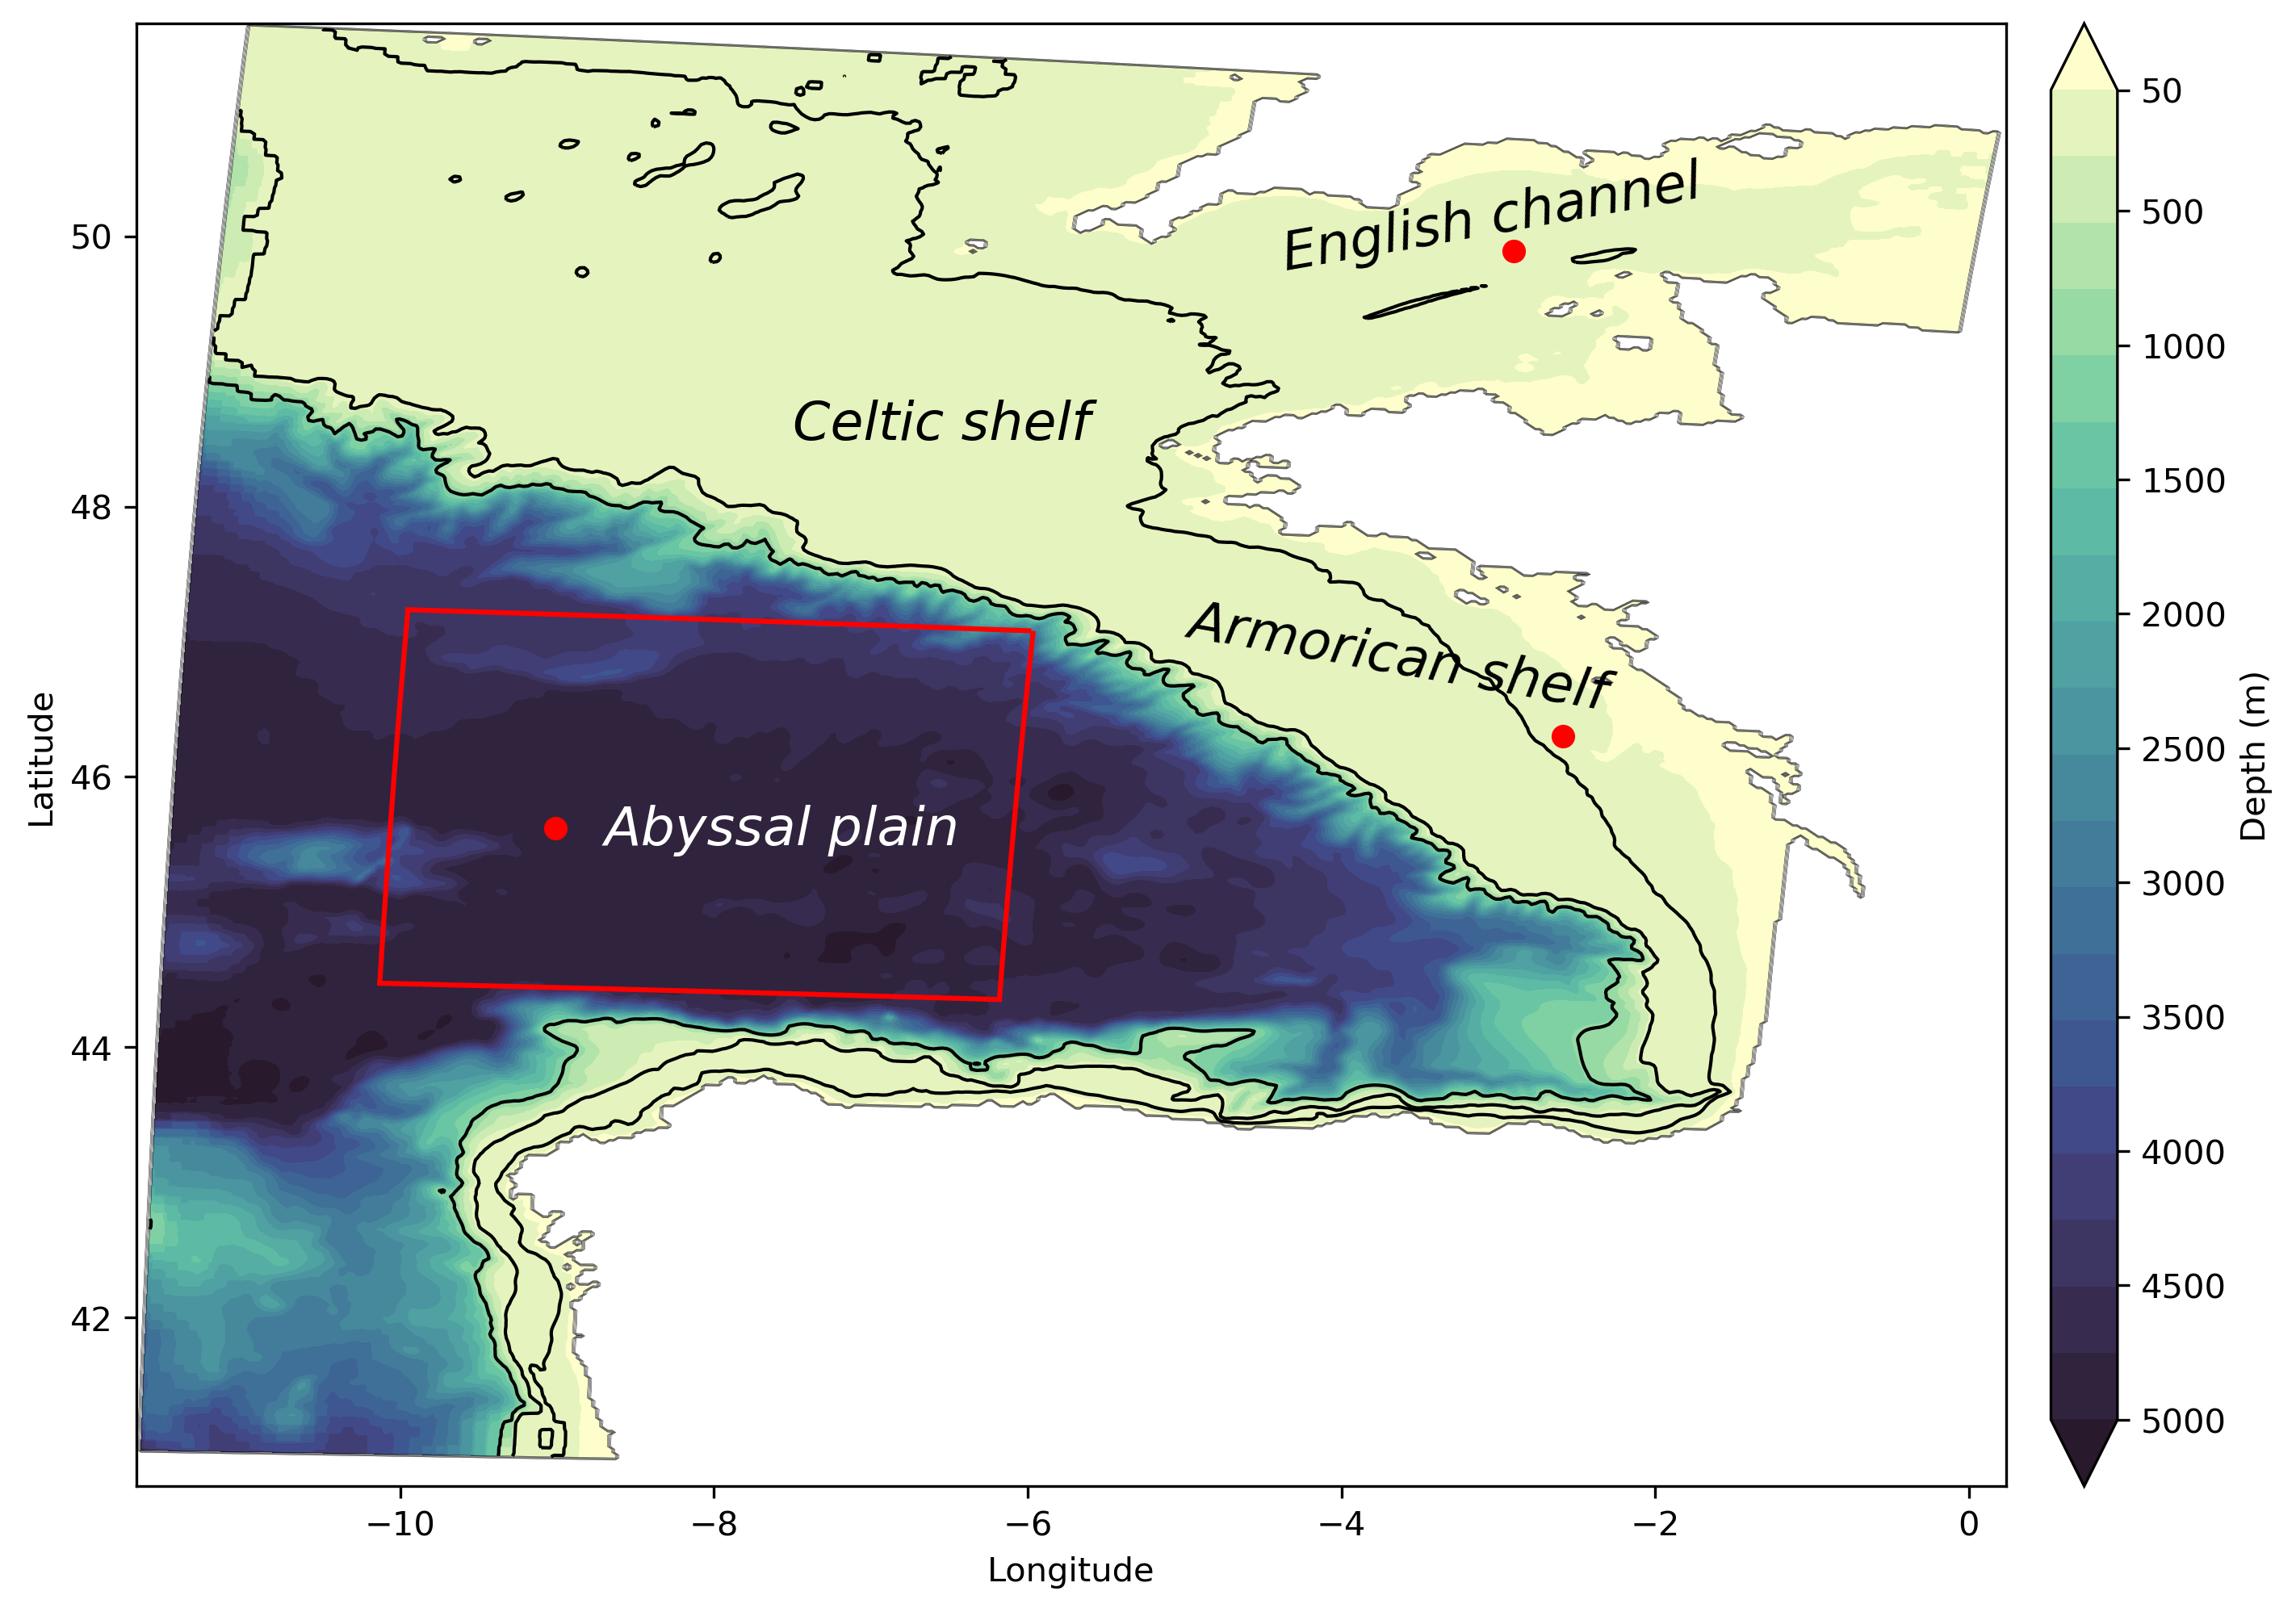
\includegraphics[width=0.7\textwidth]{Definitions/figure1.png}
    \caption{\textls[-25]{Bathymetry of the Bay of Biscay configuration in meters. The red box and dots depict the area and stations calculating model diagnostics. The black lines represent the 100, 200 and 1000 m~isobaths.}}
    \label{fig:bathymetry}
\end{figure}

%%%%%%%%%%%%%%%%%%%%%%%%%%%%%%%%%%%%%%%%%%
\subsection{Design of the Twin-Experiment}
\label{section:2.2}

We carried out a twin-experiment consisting of two simulations: (a) one with a tidal forcing (hereafter, tides-on: TON) and (b) one without tidal forcing (hereafter, tides-off: TOFF) for a period of one year from July 2011 to June 2012. The tidal motion in the TON experiment is induced in the model by both tidal potential and open boundary conditions. Other than that, the two simulations have identical atmospheric forcing, initial conditions, and the slow components of open boundary conditions of the thermohaline properties and velocities. We note that both simulations have identical model set-up for the bottom drag coefficient and the vertical mixing scheme, with the only difference being the vertical velocity shear and the stretching of the water column, when tides are activated in the model. The prognostic model variables are stored at hourly intervals for both simulations to assess the high-frequency motions due to tides.

%%%%%%%%%%%%%%%%%%%%%%%%%%%%%%%%%%%%%%%%%%
\subsection{Methodology}
\label{section:2.3}

As a first step, we analysed model outputs from the TON and TOFF simulations, comparing the model prognostic variables and other diagnostics, such as the relative vorticity, the flow divergence and the Brunt-V\"ais\"al\"a frequency, between the two simulations. In a second step, we performed spectral analysis both in frequency and wavenumber domain to quantitatively assess the impact of tides on the spectral characteristics of the Bay of Biscay dynamics.

A quantification of the water column structure can be provided by the Brunt-V\"ais\"al\"a frequency $N^2$, computed by the polynomial expression of~\cite{McDougall1987} as follows,
\begin{equation}
N^2(T,S) = -\frac{g}{\rho}\frac{\partial \rho}{\partial z} \approx g\alpha\frac{\partial T}{\partial z} -g\beta\frac{\partial S}{\partial z}
\label{eq:bn2}
\end{equation}
where $a$ is the thermal expansion coefficient; $b$ is the haline contraction coefficient; $g$ is the gravity field; $T$ and $S$ are the potential temperature and salinity profiles, respectively; and $z$ is the depth. For the calculation of the Brunt-V\"ais\"al\"a, the relative vorticity $\zeta$ = ($v_{x} - u_{y}$) and flow divergence $\sigma$ = ($u_{x} + v_{y}$) diagnostics, we used the CDFTTOOLS package (\url{https://github.com/meom-group/CDFTOOLS}). 

A Fast Fourier Transform analysis for the Sea Surface Height (SSH) variance was performed to estimate the energy spectrum as a function of frequency. A Welch filter~\cite{welch1967} and a temporal Hanning window of approximately 2 days was applied to hourly segments, to remove noise and highlight the dominant spectral peaks. The calculations were performed for the two simulations and over typical locations shown in Figure~\ref{fig:bathymetry}, i.e.,~stations depicted with red dots in the abyssal plain, Armorican shelf and the English Channel.

The energy associated with motions of different spatial scales was quantified using a wavenumber spectral analysis. We used the pyspec package (\url{https://github.com/pyspec/pyspec}) to estimate the horizontal isotropic wavenumber spectrum~\cite{Rocha2016} from the model hourly fields in a subdomain spanning the abyssal plain 6.1$^{\circ}${--}10.1$^{\circ}$ W, 44.4$^{\circ}${--}47.2$^{\circ}$ N (Figure~\ref{fig:bathymetry}; red box). The selected subdomain includes spatially homogeneous ocean circulation patterns constrained in the abyssal plain by the continental slope. The spectral method incorporates a two-dimensional Discrete Fourier Transform, applying also a spatial smoothing Hanning window of an order of 3 km and removing the spatial averages. The~spectrum was azimuthally averaged per wavenumber~\cite{Rocha2016}.

\textls[-25]{As proposed in~\cite{simpson1974}, we also calculated the tidal mixing parameter (referred as the Simpson--Hunter parameter; hereafter SH) to identify the location of tidal fronts and intense tidal~mixing: }
\begin{equation}
SH = log_{10}(h/U^3)
\label{eq:SH}
\end{equation}
where $h$ is the water depth in meters and $U$ is the depth-averaged tidal velocity in $m/s$. According to the authors of~\cite{simpson1974}, the fronts should be located in areas with a critical SH parameter value. These SH values can be used to identify specific areas of intense tidal mixing. By definition, the SH parameter is estimated when tides are included in the model (i.e.,~here the TON simulation). When SH values are small, there is a homogenisation of the water column, in particular in regions dominated by strong tidal currents~\cite{simpson1981}. For the Northwest European shelf, and specifically in the English Channel, the~critical SH values reported in the literature~\cite{bowerS1987,holt2008} are between 2.7 and 3.0. In the results section, the SH parameter computed over the summer period is also compared to the temperature difference between surface and bottom waters (i.e.,~$\Delta T=T_{surface}-T_{bottom}$), to highlight areas of intense tidal mixing.

%%%%%%%%%%%%%%%%%%%%%%%%%%%%%%%%%%%%%%%%%%
\section{Results}
\label{section:3}

In this section, we investigate the impact of tidal forcing on the Bay of Biscay by comparing the results of the two model simulations (TON and TOFF). We consider the differences in the thermohaline properties, the circulation patterns and the evolution of the stratification in different areas of the domain. Finally, we perform spectral analysis of the SSH evolution, in order to identify the impact of tides on the energy distribution at different time and spatial scales.

As an illustration of the tidal forcing applied in the TON simulation (and excluded from the TOFF simulation), we present in Figure~\ref{fig:tidal_constituents} the amplitude and phase of M2 and M4 tidal constituents. M2~is the major tidal constituent in the Northeast Atlantic Ocean with amplitudes exceeding 3 m in the domain (Figure~\ref{fig:tidal_constituents}a). M4 is a principal quarter-diurnal compound tide generated from the interaction of M2 with itself. The M4 amplitude is more significant over the continental shelf than the abyssal plain, with maximum amplitudes localised in the Armorican shelf and the English Channel (Figure~\ref{fig:tidal_constituents}b). The~tidal map of M4 shows two amphidromic points (zero amplitude) located in the English Channel as described by~\cite{LeProvost1985}.

\begin{figure}[H]
    \centering
    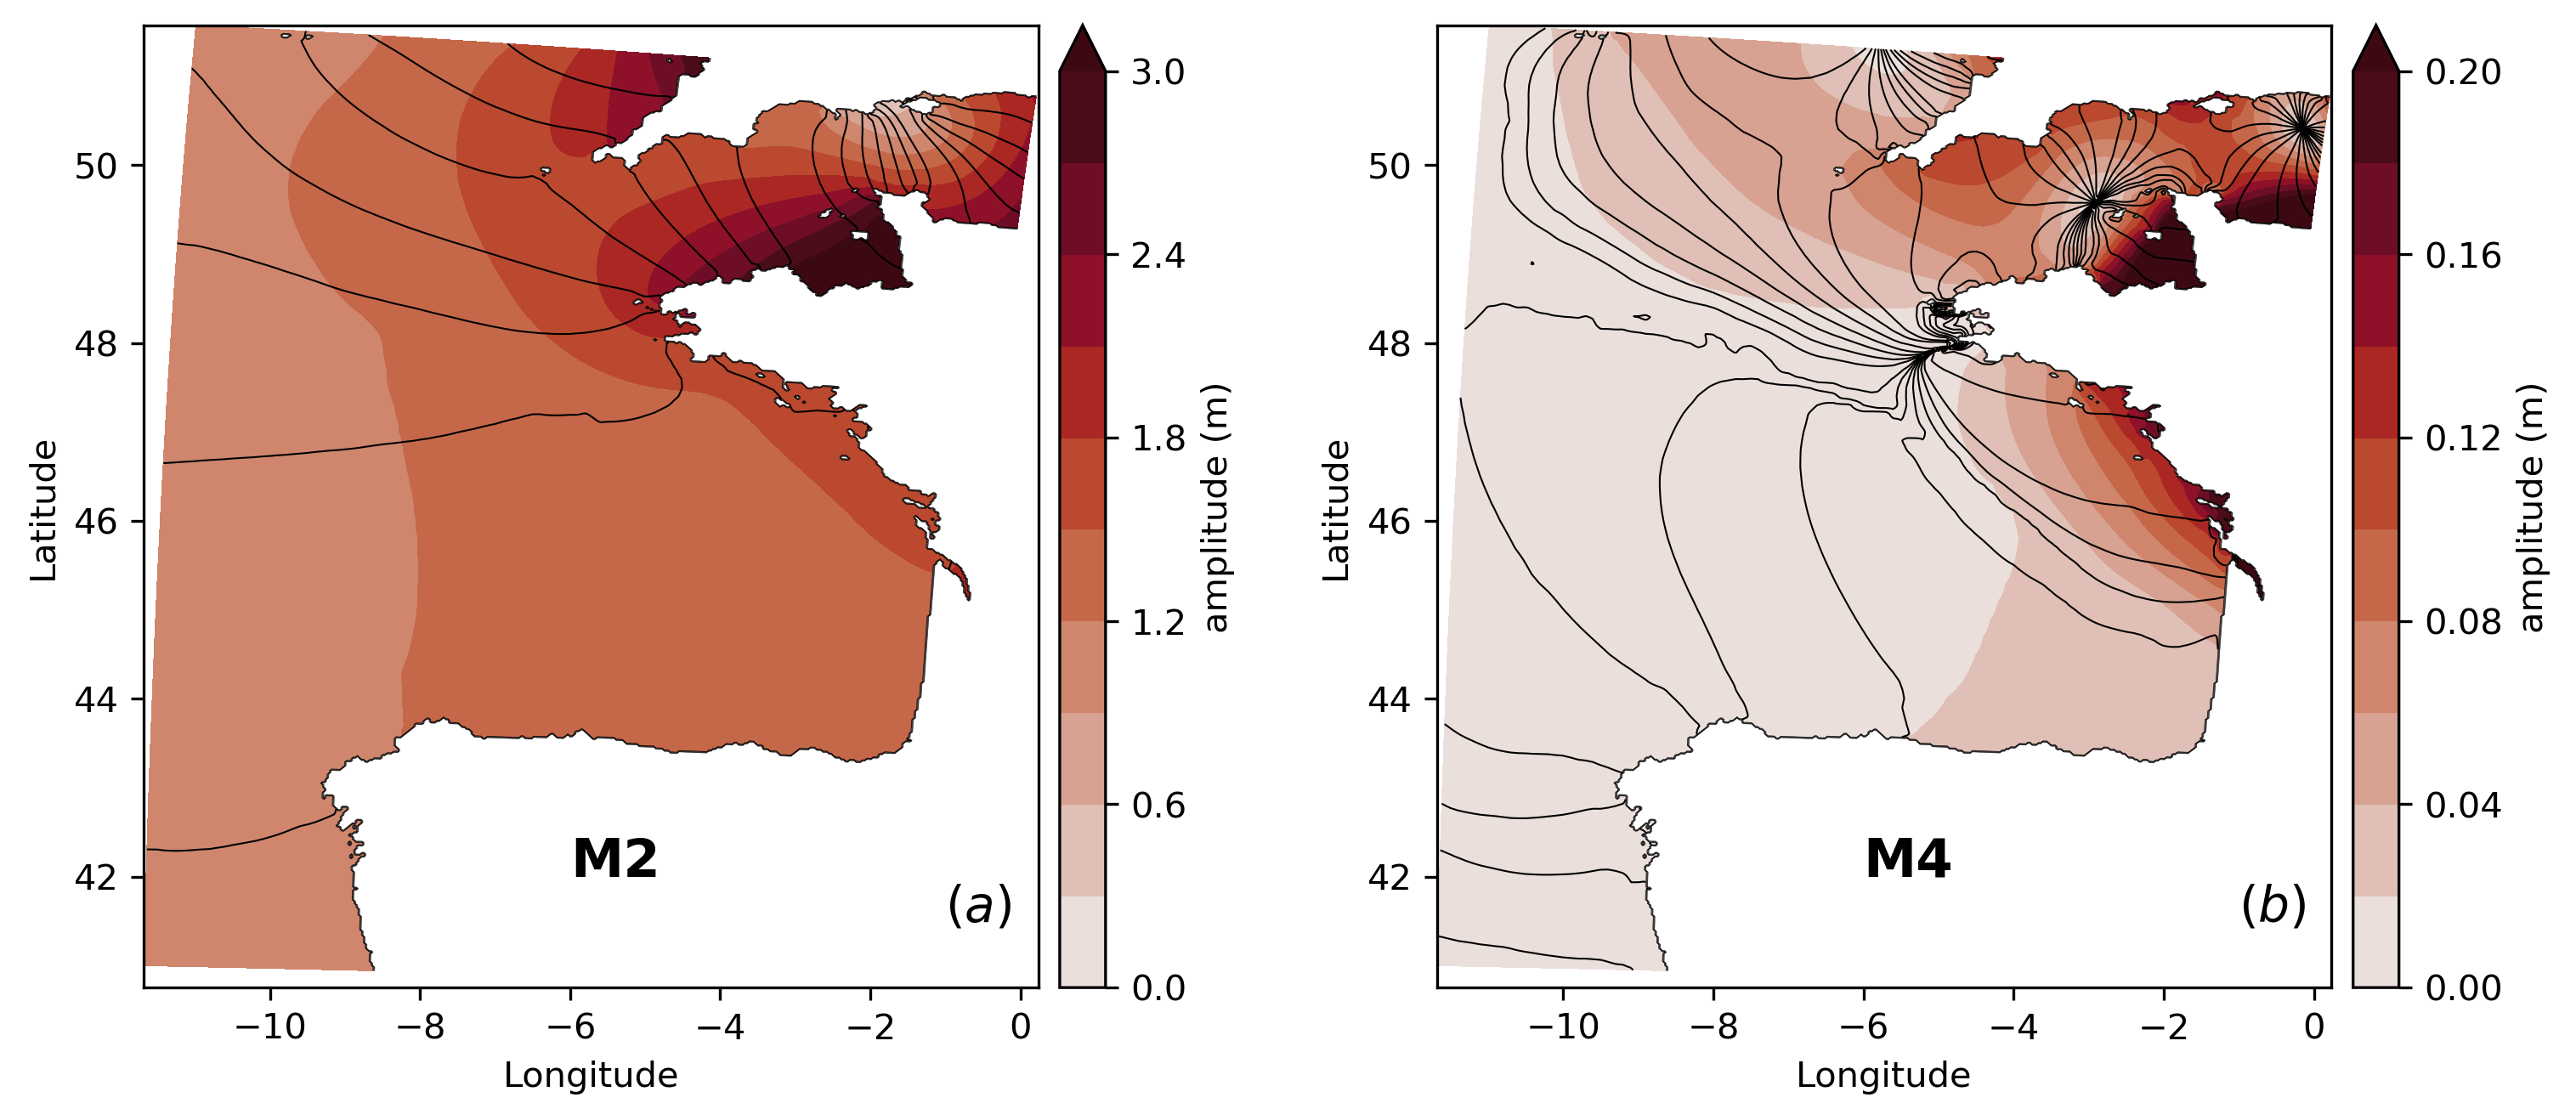
\includegraphics[width=0.8\textwidth]{Definitions/figure2.png}
    \caption{Amplitude in meters (colour) and phase (black lines; amphidromic points: zero amplitude) of modelled (\textbf{a}) M2 and (\textbf{b}) M4 tidal constituent.}
    \label{fig:tidal_constituents}
\end{figure}

%%%%%%%%%%%%%%%%%%%%%%%%%%%%%%%%%%%%%%%%%%
\subsection{Distribution of Thermohaline Properties}
\label{section:3.1}

Figures~\ref{fig:ostia}--\ref{fig:sss} present the observational data OSTIA~\cite{donlon2012} and the modelled Sea Surface Temperature (SST) and Salinity (SSS), respectively. The data and model results are illustrated for two representative days at the end of summer (upper panels) and in mid-winter (lower panels). In Figures~\ref{fig:sst} and \ref{fig:sss}, the left panels correspond to the TON simulation, the middle panels to the TOFF simulation and the right panels to their difference ``TON minus TOFF''. In summer, both simulations reproduce the characteristic ``warm pool'' in the southeastern corner of the Bay of Biscay (Figure~\ref{fig:sst}a,b), with SST values exceeding 20 $^\circ$C verified also by the OSTIA-SST satellite observations (Figure~\ref{fig:ostia}a). During the same period and over the Celtic and Armorican shelves, we observe the Ushant tidal front at the entrance of the English Channel ($48.2^\circ$ N, $5.6^\circ$ W) in the OSTIA-SST dataset and only in the realistic TON simulation; we~observe cold waters at about $15^\circ$C in the vicinity near the coasts and warmer waters outside the front (Figures~\ref{fig:ostia}a and~\ref{fig:sst}a). During winter, there is a marked spatial variability in hydrography with warmer and generally saltier waters in the open ocean compared with the shelves (i.e.,~by approximately 12{--}%we changed hyphen to en-dash, please confirm.
13~$^\circ$C and 35.6{--}35.8; Figures~\ref{fig:ostia}b,~\ref{fig:sst}d and~\ref{fig:sss}d). A thermal front observed in the OSTIA-SST and in both simulations during winter, separates the coastal cold waters (i.e.,~values do not exceed 10~$^\circ$C) of the Armorican shelf influenced by the river plumes, with the open ocean warm waters. The~same period, in the abyssal plain, we observe the presence of coherent eddies and filaments in both simulations, leaving a clear imprint of the circulation pattern on the SST and SSS fields (Figures~\ref{fig:sst}d,e and~\ref{fig:sss}d,e) in contrast with the smoothed OSTIA fields (Figure~\ref{fig:ostia}b). When we validate the model with in situ observations at the Channel Lightship station ($49.9^\circ$ N $2.9^\circ$ W; \url{https://marine.copernicus.eu}; Figure~S1), we find that the TON simulation has smaller Mean Absolute Error (MAE) at about $0.59$ $^\circ$C over the simulation period, as opposed to the TOFF experiment with MAE $0.85$ $^\circ$C.

\begin{figure}[H]
    \centering
    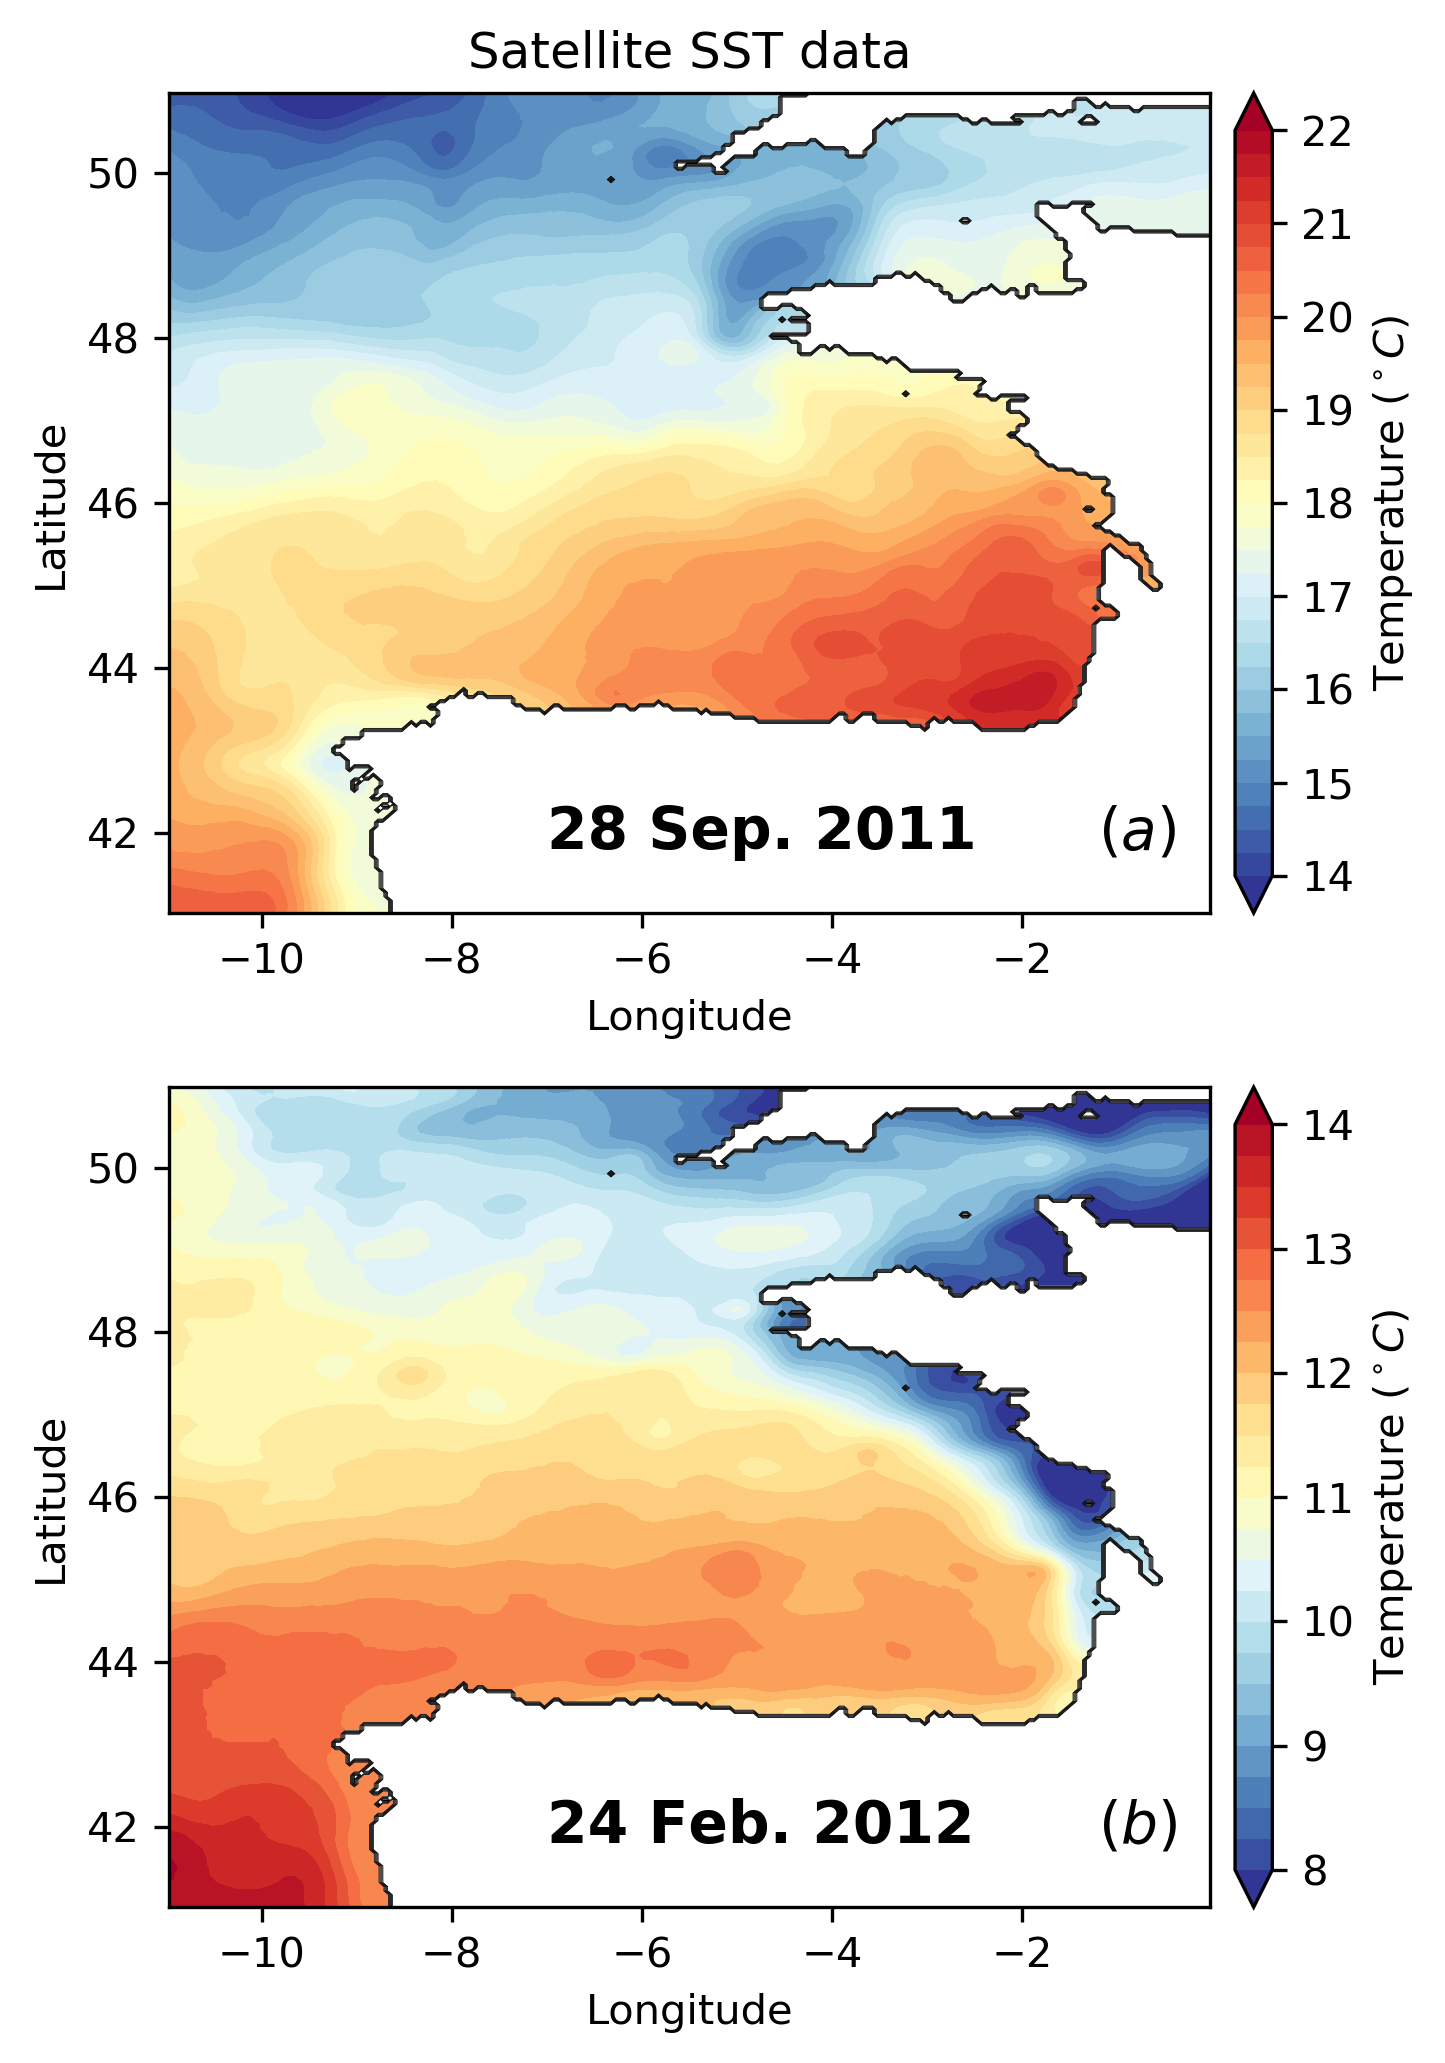
\includegraphics[width=0.4\textwidth]{Definitions/figure3.png}
    \caption{Sea surface temperature ($^\circ$C) from OSTIA L4 satellite observations on (\textbf{a}) 28 September 2011 and (\textbf{b}) 24 February 2012.}
    \label{fig:ostia}
\end{figure}
 
Differences in SST between TON and TOFF simulations suggest that the addition of tidal forcing produces high spatial changes of SST locally exceeding $1$ $^\circ$C (Figure~\ref{fig:sst}c,f). The tidal forcing contribution to the SST fields is different in the two periods. For example, during summer, the SST is colder when tides are activated, while the opposite is true during the winter period (Figure~\ref{fig:sst}c,f). In summer, the~SST is colder in TON compared with the TOFF simulation in the English Channel, the shelves (near the continental shelf break at approximately $47 ^\circ$ N) and in the Spanish continental slope at approximately $43.5 ^\circ$ N (Figure~\ref{fig:sst}c). The largest temperature differences are locally observed in the position of the Ushant front, which is formed only in the TON simulation (Figure~\ref{fig:sst}a--c). The latter result is of substantial importance as oceanic fronts play a key role in the circulation of shelf seas which are regions of intense biological activity. Another finding is that the northern coast of the English Channel has warmer SSTs than the rest of the Channel when tides are activated, which can affect the ocean model's skill to represent the SST compared to satellite observations (cf.~\cite{TIMKO2019}).

Examining the differences in winter, the SST is warmer when tides are activated, notably in the English Channel and in the largest part of the abyssal plain (Figure~\ref{fig:sst}f). In the Armorican shelf, we observe small-scale contrasting positive--negative SST fields for the difference ``TON minus TOFF'' (i.e.,~differences up to 1 $^\circ $C), attributed on the frontal displacement of the river plumes. The latter is also in agreement with the coastal SSS fields modulated by the river plumes (Figure~\ref{fig:sss}f). In the same area, along the continental slope at about $4 ^\circ$ W to $9 ^\circ$ W, the SST appears to be colder in the simulation with tides than without tides. This SST cooling is less intense compared with values observed during summer (Figure~\ref{fig:sst}c). This cooling is most likely associated with internal tides breaking in the continental slope and subsequently enhancing mixing in the shelves, bringing cold bottom waters on the surface (cf. also~\cite{PINGREE1995}). 

\begin{figure}[H]
    \centering
    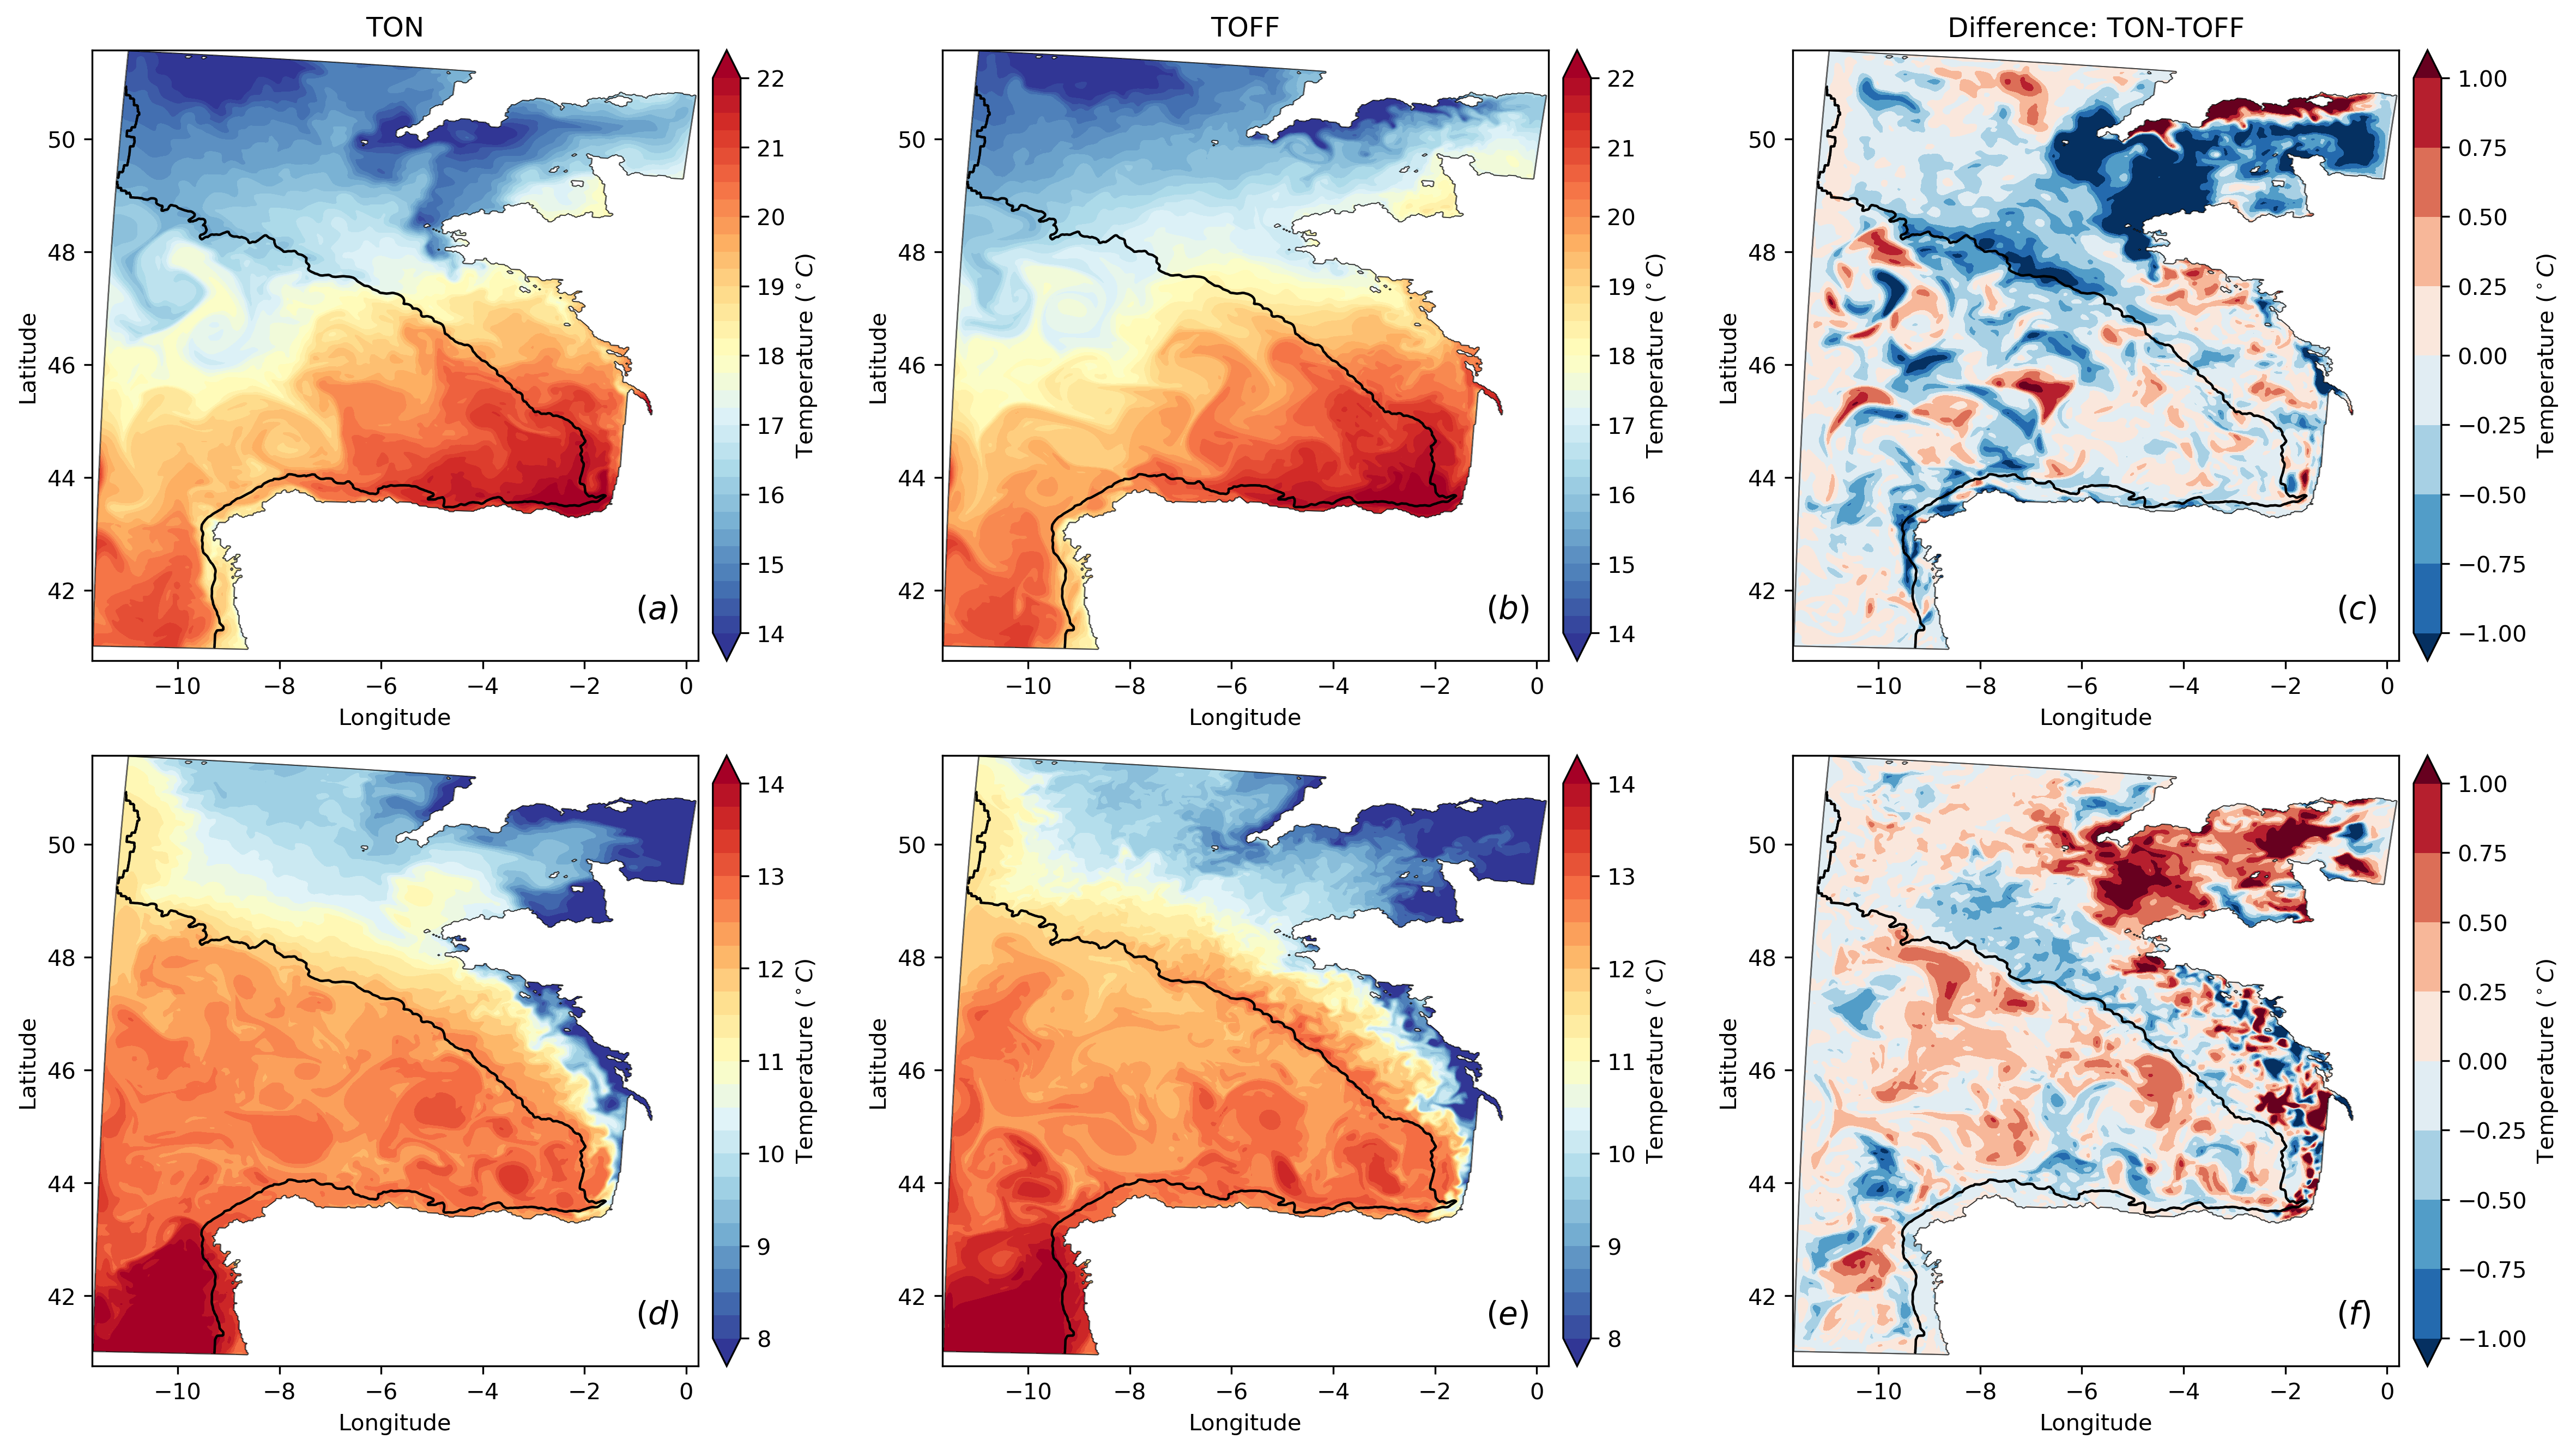
\includegraphics[width=0.95\textwidth]{Definitions/figure4.png}
    \caption{Sea surface temperature ($^\circ$C) on (\textbf{a}--\textbf{c}) 28 September 2011 and (\textbf{d}--\textbf{f}) 24 February 2012 for tides-on (TON) and tides-off (TOFF), and their difference ``TON minus TOFF'', respectively. The black line indicates the 200-m isobath, which delimits the shelf break.}
    \label{fig:sst}
\end{figure}
\unskip
\begin{figure}[H]
    \centering
    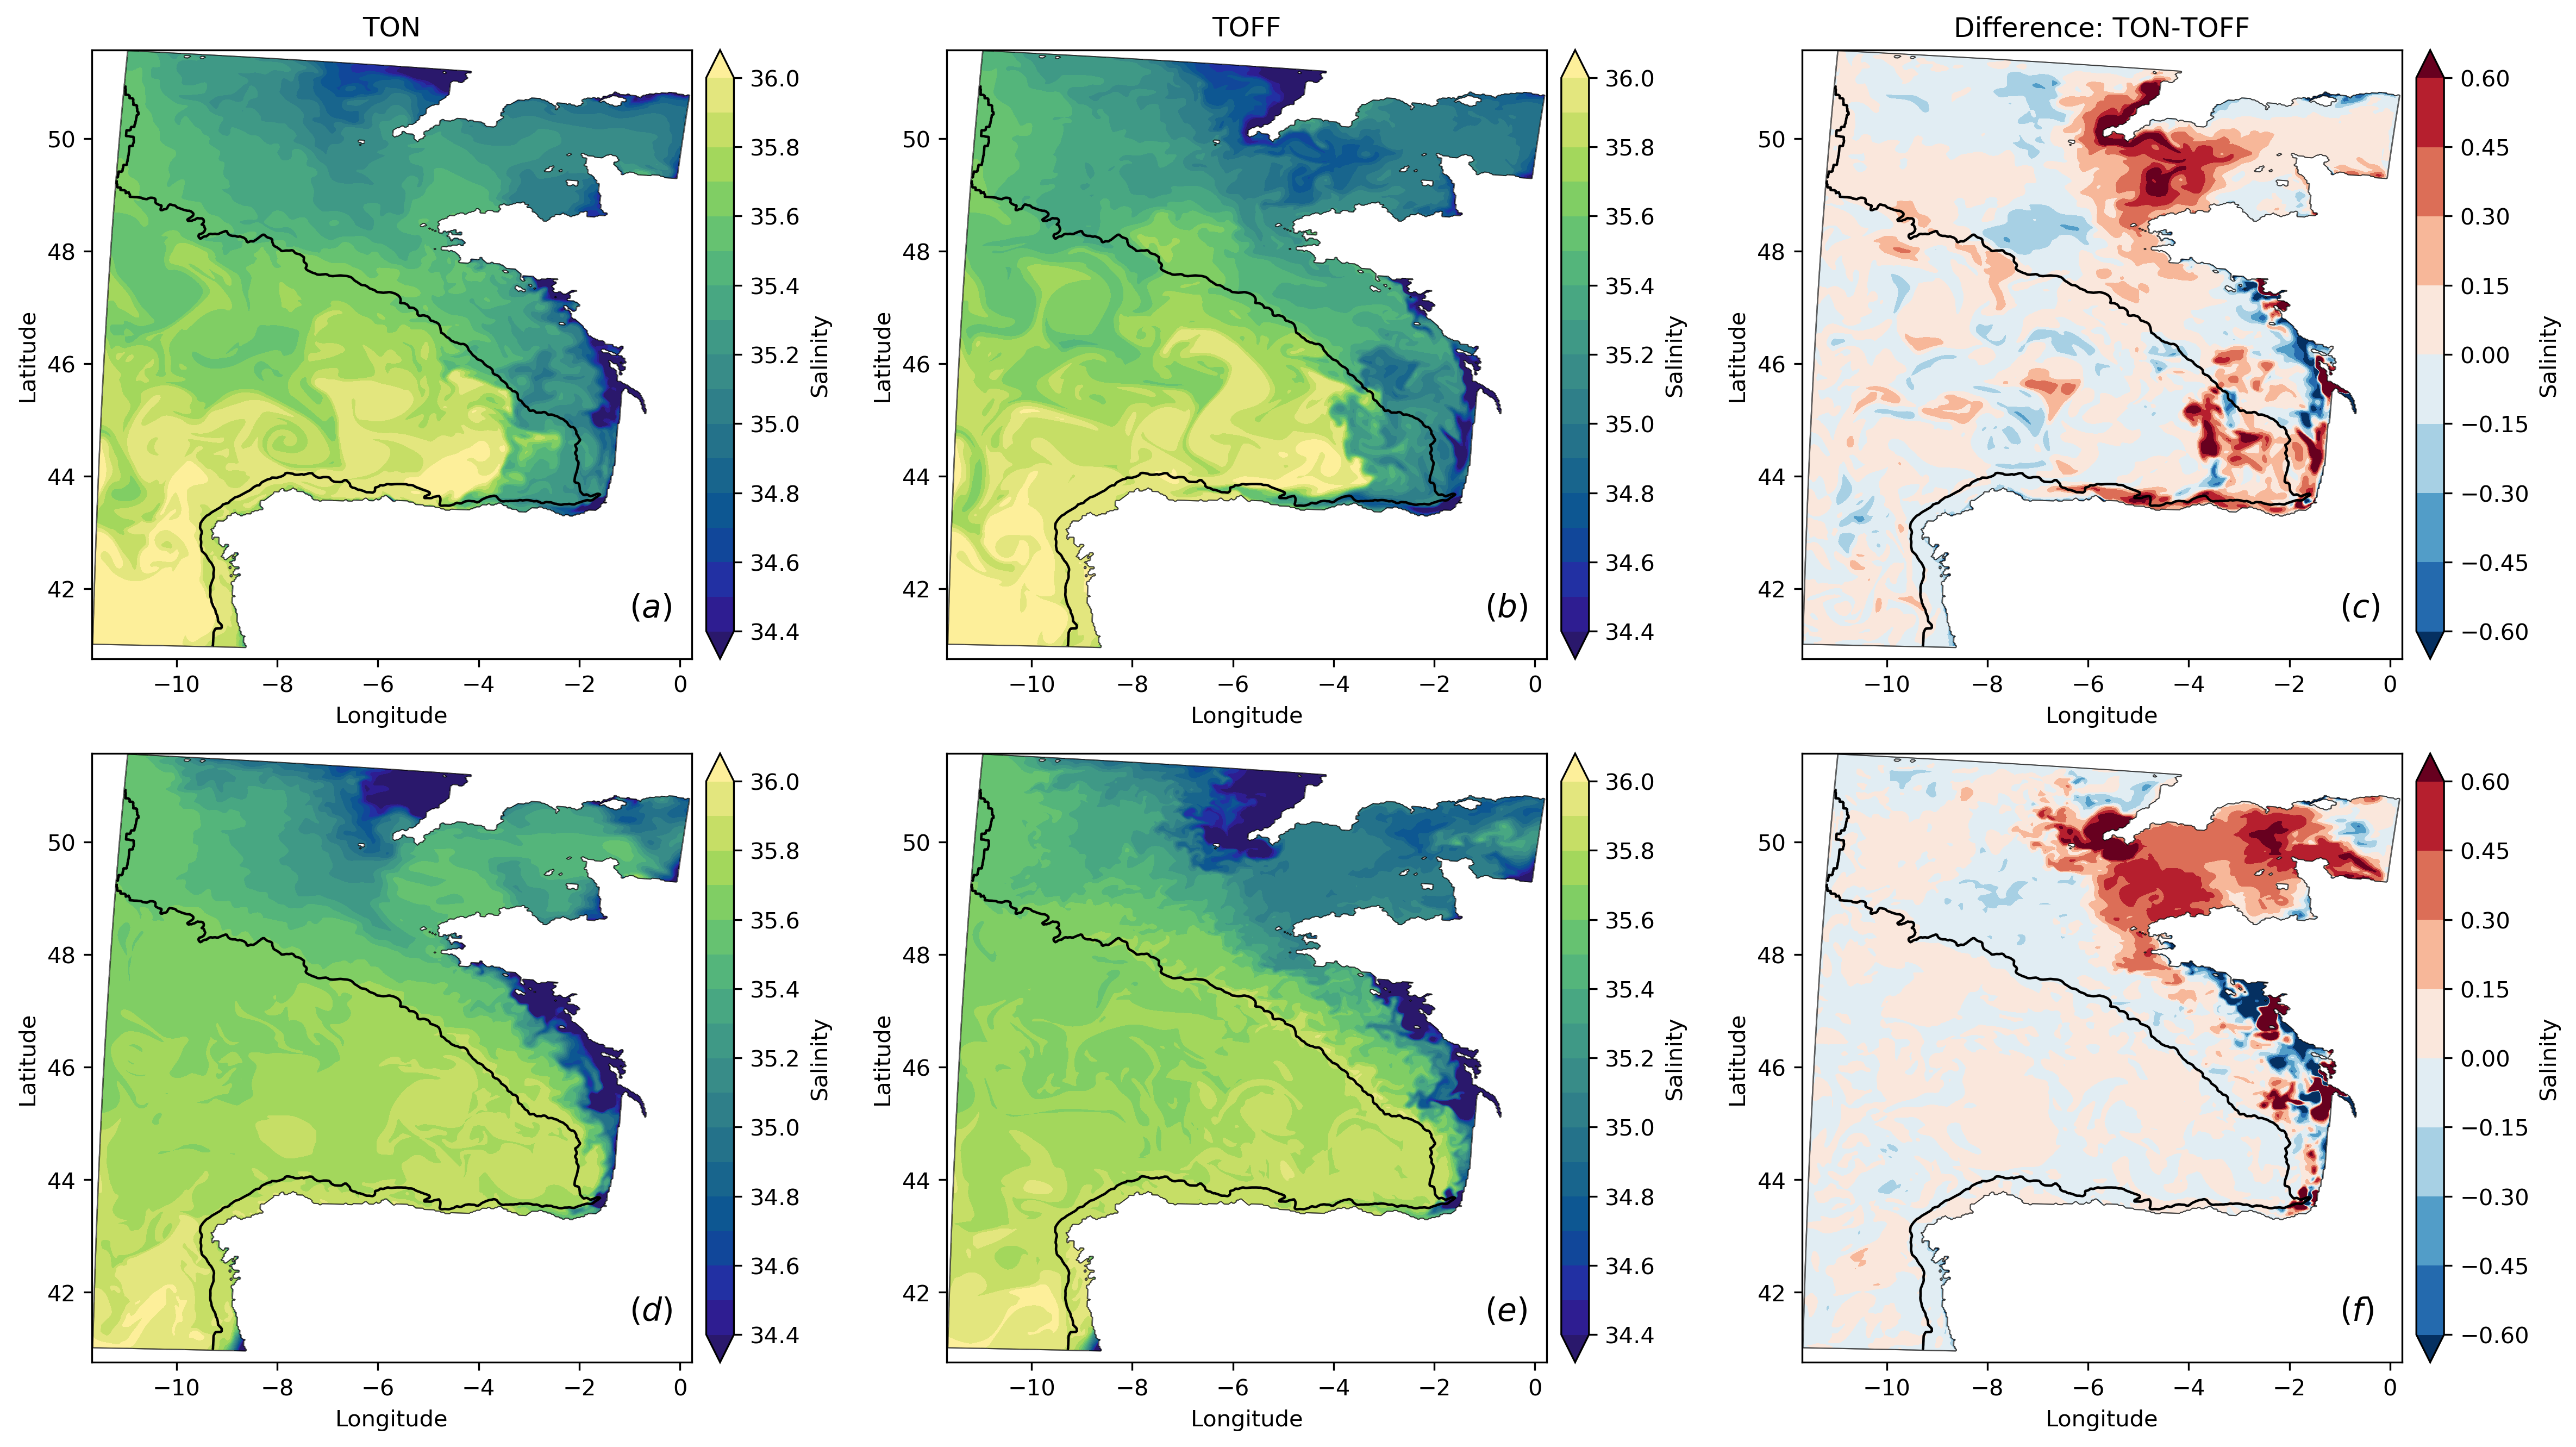
\includegraphics[width=0.95\textwidth]{Definitions/figure5.png}
    \caption{{Same }%Please add explanations for all subfigures in the caption.
     as Figure~\ref{fig:sst} for the sea surface salinity.}
    \label{fig:sss}
\end{figure}

In Figure~\ref{fig:sss}c,f, we present the differences in SSS between the two simulations and the two periods. The greatest differences are observed in the English Channel (i.e.,~greater than 0.6), most notably in the entrance of the Channel (near $48.5^\circ$ N, $4^\circ$ W). This is possibly explained by the fact that the Ushant front acts as a barrier to the intrusion of low salinity waters (i.e.,~values < 35.2; cf.~\cite{Kelly-Gerreyn2006}), originated from the Loire and Gironde rivers. We note that the SSS increases (in both periods) in the English Channel when tides are activated, in contrast to SST which only increases in the TON simulation and only during the winter. The rivers freshwater transport from the shelves to the open ocean is constrained when tides are activated in the model simulation, probably due to changes in stratification and mixing (discussed in Section~\ref{section:3.3}). This pattern is observed during summer, when occurring high salinity differences (i.e.,~values up to 0.6) in the transition area of the Landes Plateau at approximately $44.5^\circ$ N, $3.5^\circ$ W (Figure~\ref{fig:sss}c).

Figure~\ref{fig:ushant}a,b shows the temperature difference between the surface and bottom waters during summer for the TON and TOFF simulations. As shown in Figure~\ref{fig:ushant}a, the English Channel is an area characterised by intense tidal mixing, illustrated by $\Delta T$ with values lower than $0.5$ $^\circ$C. The location of the Ushant front can be identified by the $\Delta T$ isotherm of $0.5$ $^\circ$C (Figure~\ref{fig:ushant}a; black line) and the area spanned by the 2.7 and 3.0 contours of the Simpson--Hunter parameter (Figure~\ref{fig:ushant}a; magenta lines). In the simulation without tides, $\Delta T$ has greater values than the $0.5$ $^\circ$C threshold (e.g.,~up to $7$ $^\circ$C) confirming the absence of fronts in the area (Figure~\ref{fig:ushant}b). Figure~\ref{fig:ushant}c presents the longitudinal cross section of the water column temperature near the entrance of the English Channel. The cross section was selected in the area where the $\Delta T$ isotherm of $0.5$ $^\circ$C and the SH contours are collocated, denoting the presence of the Ushant tidal front (Figure~\ref{fig:ushant}a). We observe a homogenisation of the water column east of $5.4^\circ$~W (Figure~\ref{fig:ushant}c). On the contrary, in the simulation without tides, we observe a well-formed seasonal thermocline at approximately 40 m depth (Figure~\ref{fig:ushant}d).

\begin{figure}[H]
    \centering
    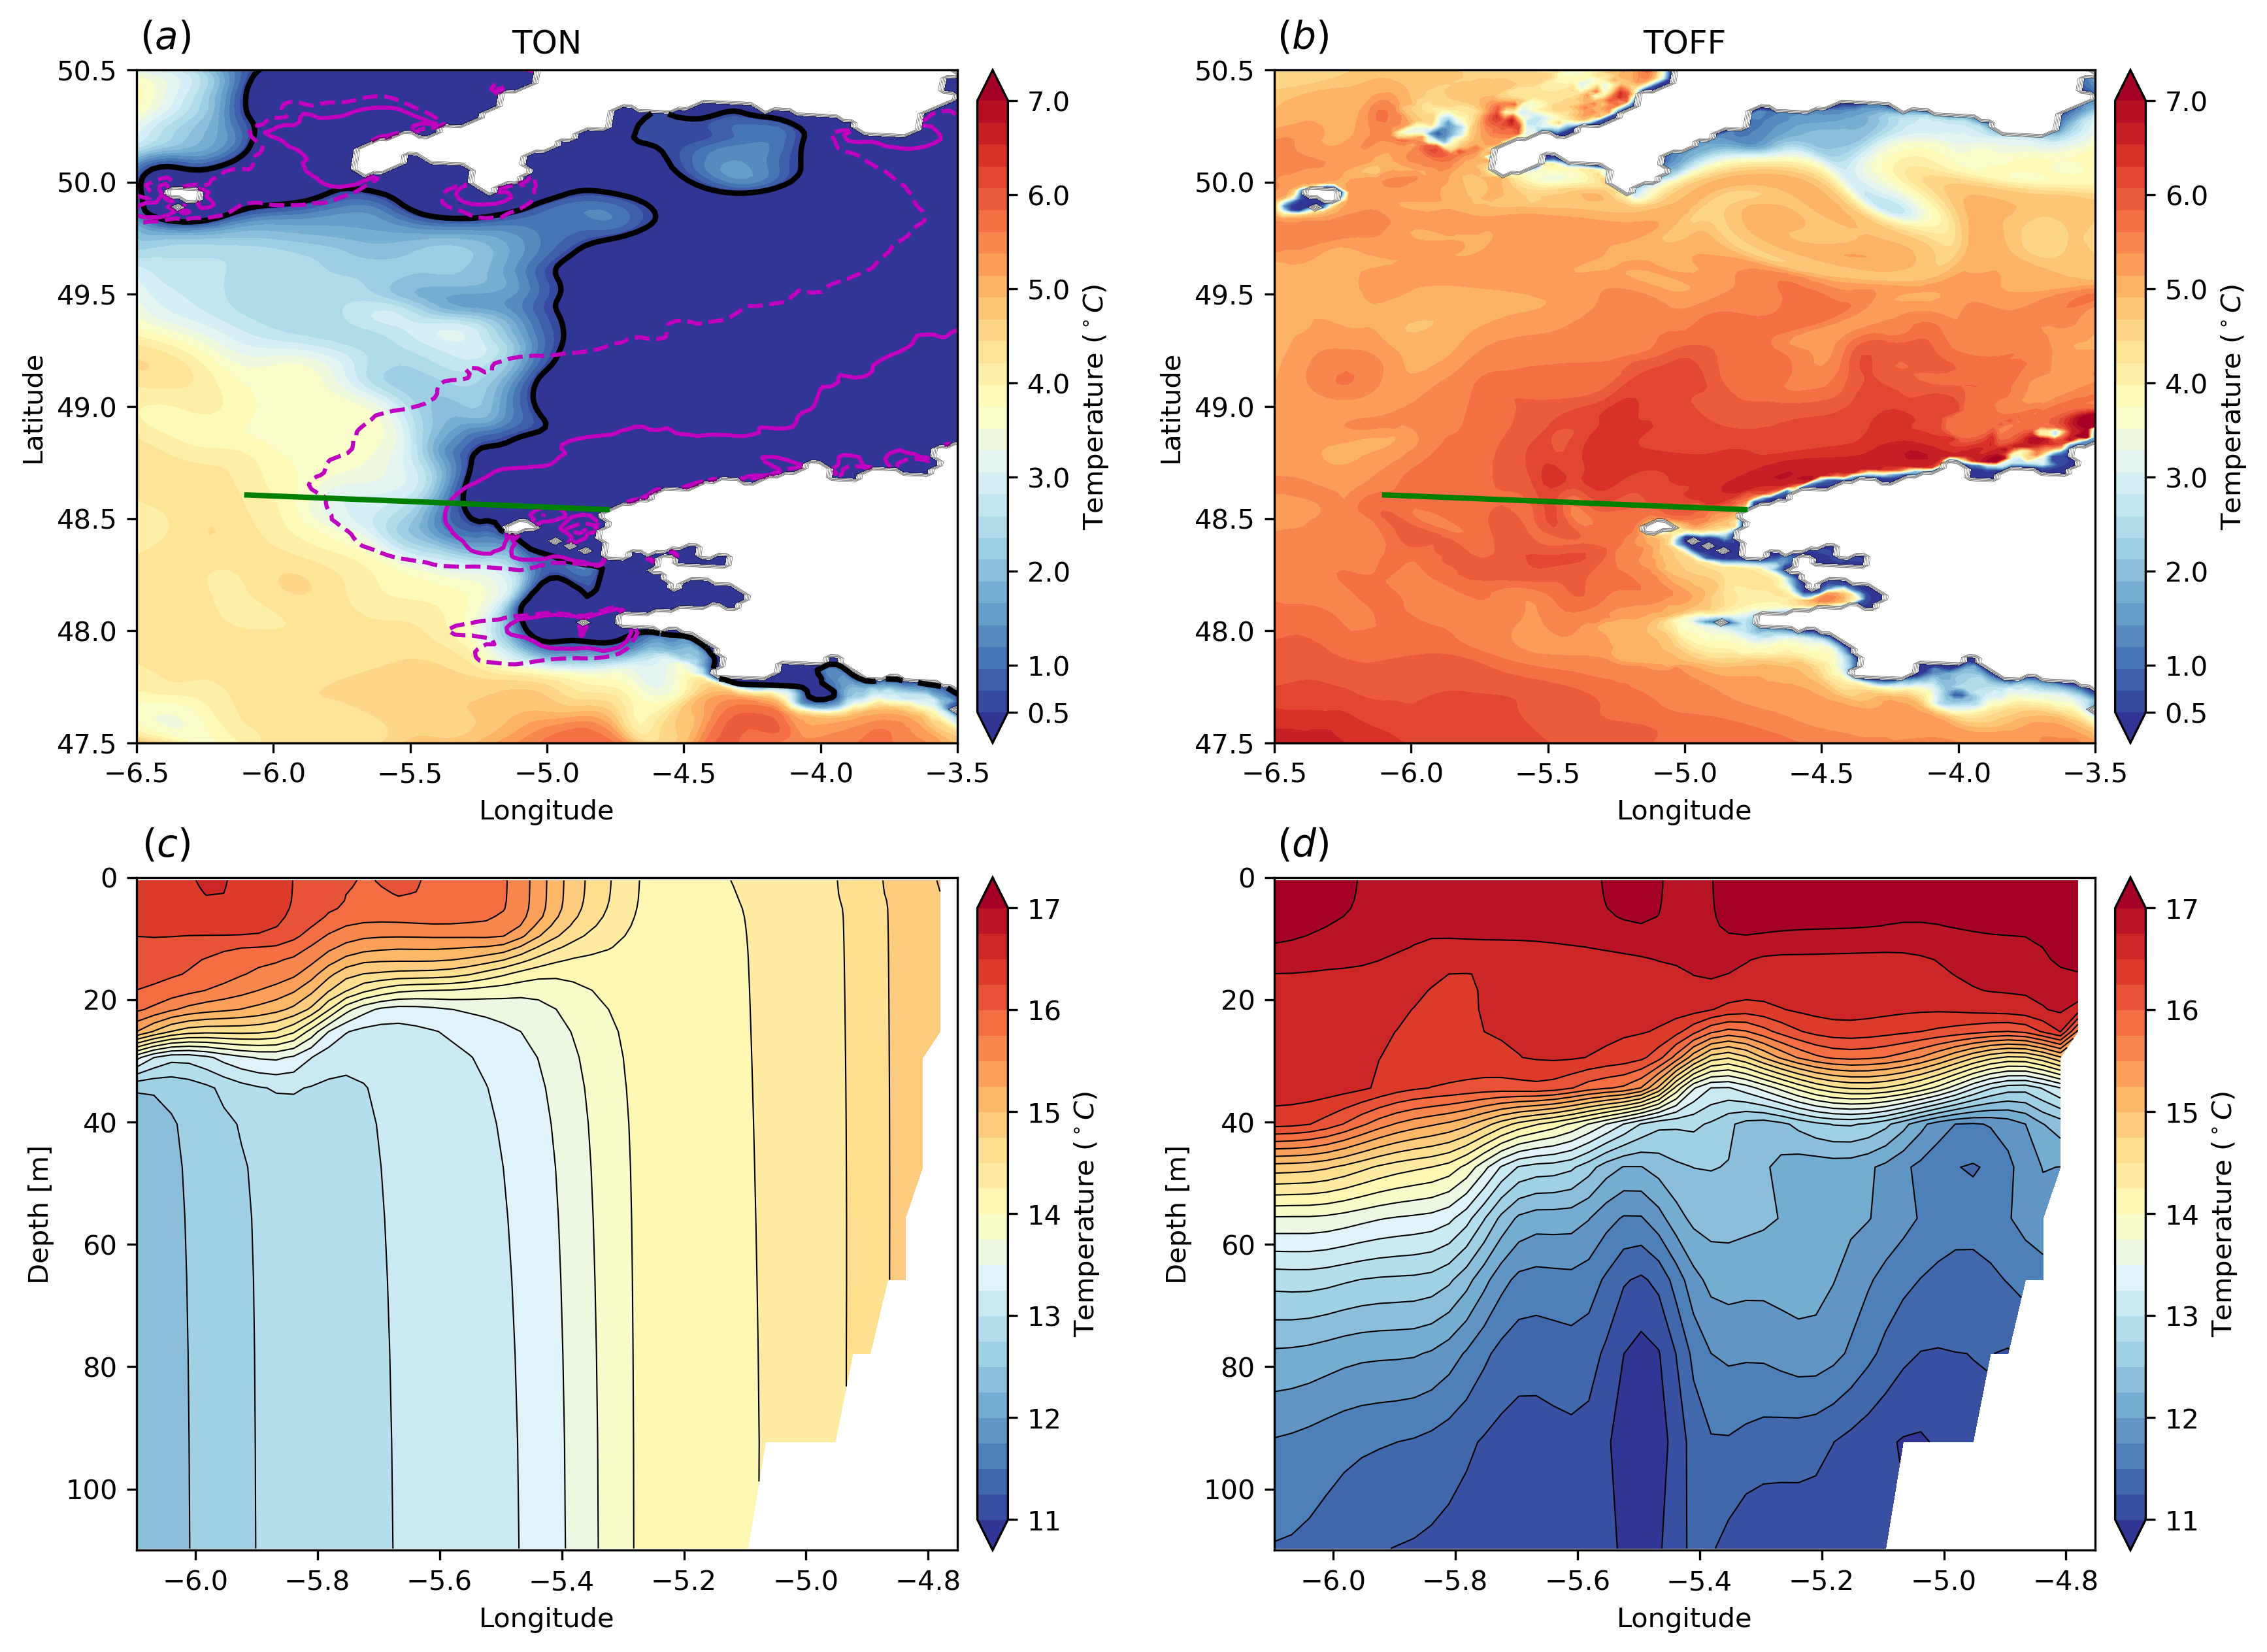
\includegraphics[width=0.95\textwidth]{Definitions/figure6.png}
    \caption{(\textbf{a},\textbf{b}) Surface minus bottom temperature on 28 September 2011 for TON and TOFF in a zoom area near the entrance of the English Channel. (\textbf{c},\textbf{d}) Vertical cross sections of temperature along green lines shown in subplots (\textbf{a},\textbf{b}). The magenta lines in subplot (a) present the values of Simpson--Hunter parameter for the contours of 2.7 (solid) and 3.0 (dashed) respectively, and the solid black line the contour of $\Delta T=0.5$ $^\circ$C.}
    \label{fig:ushant}
\end{figure}
%%%%%%%%%%%%%%%%%%%%%%%%%%%%%%%%%%%%%%%%%%
\subsection{Relative Vorticity and Divergence}
\label{section:3.2}

In this section, we investigate the relative vorticity and surface divergence fields to assess the dynamical impact of tides on the Bay of Biscay mesoscale activity. In Figure~\ref{fig:vorticity}, we depict the relative vorticity, with and without tides, for the same dates as in the SST and SSS fields. As expected, during winter, we observe in both simulations more intense circulation patterns in the abyssal plain compared with the summer circulation, attributed to coherent and more energetic eddies and vortices constrained in the abyssal plain by the continental slope. 

\begin{figure}[H]
    \centering
    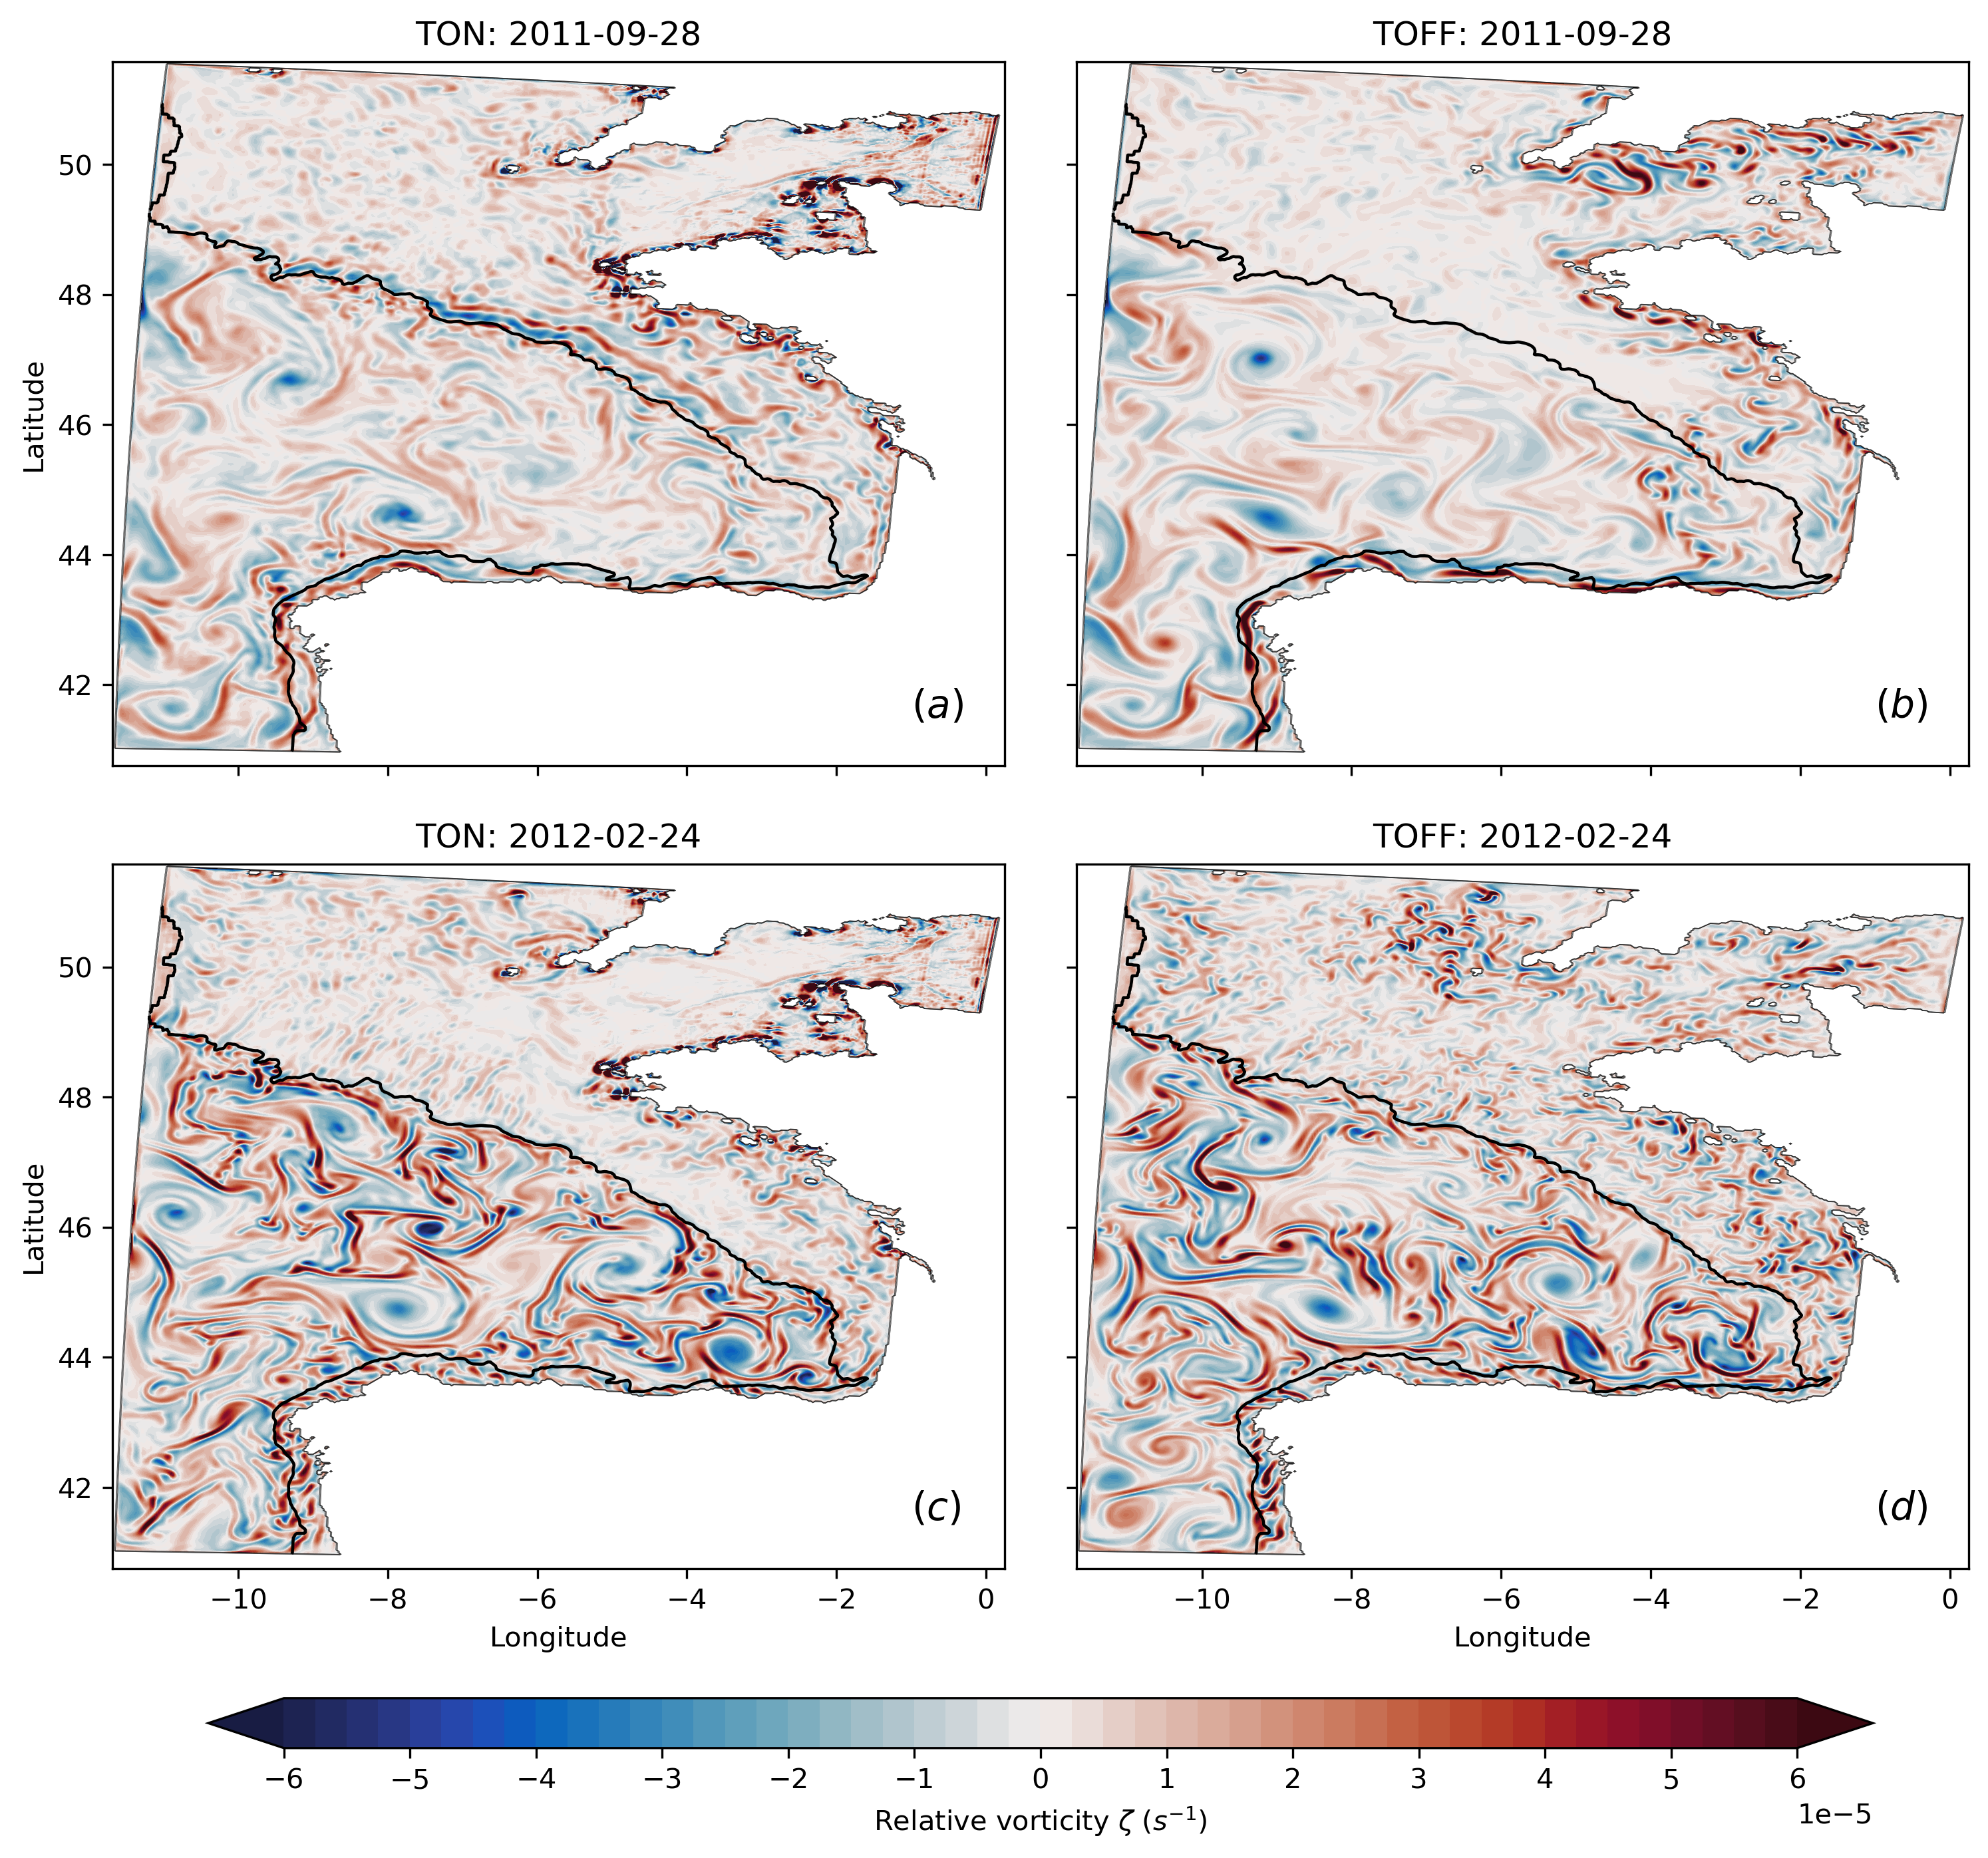
\includegraphics[width=0.8\textwidth]{Definitions/figure7.png}
    \caption{Surface relative vorticity ($s^{-1}$) for (\textbf{a},\textbf{b}) 28 September 2011 and (\textbf{c},\textbf{d}) 24 February 2012. Panels (a,c)~correspond to the TON simulation and panels (\textbf{b},\textbf{d}) to the TOFF simulation respectively.}
    \label{fig:vorticity}
\end{figure}

Near the shelf break and only during summer in the TON simulation, there is a crest-through signal of internal tides propagation in the Armorican and Celtic shelves at approximately $47^\circ${--}$48^\circ$~N~$5^\circ${--}$7^\circ$~W (Figure~\ref{fig:vorticity}a). During winter, when tides are activated, the relative vorticity fields present small-scale structures, especially in the Armorican shelf near the coasts and the Loire and Gironde river discharges (Figure~\ref{fig:vorticity}c).  

During summer, when tides are included in the simulation, there is a marked increase in relative vorticity over the Armorican and Celtic shelves at approximately $47^\circ${--}$48^\circ$ N and $4^\circ${--}$8^\circ$ W, compared with the TOFF simulation (Figure~\ref{fig:vorticity}b). On the other hand, during the same period, the relative vorticity is decreased in the northern part of the English Channel in the presence of tidal forcing (Figure~\ref{fig:vorticity}a,b). During winter, there are evidences of small-scale vortices over the Armorican shelf in Figure~\ref{fig:vorticity}d (TOFF simulation), confirmed also previously by the winter temperature and salinity fields \mbox{(cf. Figures~\ref{fig:sst}e and~\ref{fig:sss}e)}. In the same period over the abyssal plain, we observe an increase of mesoscale activity southern to the shelf break in the TON simulation, i.e.,~$47^\circ$ N, $7^\circ$ W, near the generation area of internal tides (Figure~\ref{fig:vorticity}c,d). Overall, when tides are included, small-scale and mesoscale activity weakens on the shelves during both periods and increases in the open-ocean, notably southern to the shelf break and during summer when stratification is strong.

In this study, we depict also the summer divergence of the surface circulation for the TON experiment, as a means to investigate the dynamics of internal tides in our model domain (Figure~\ref{fig:divergence}). There are evidences of spatial patterns with positive/negative values of divergence flow, denoting the vertical variations in the water column as a result of internal tides. We note that, in the TOFF experiment, this divergence pattern is totally absent (i.e.,~lower values at about two orders of magnitude compared with the TON simulation; not shown). In more detail, we observe high values of divergence flow along the continental shelf slope, most notably at $47^\circ${--}$48^\circ$ N, 
$4^\circ${--}$8^\circ$ W and in agreement with the literature, characterised as a hot spot area of internal tides generation, due to the interaction of barotropic tides with the steep slope~\cite{Pingree1986,PINGREE1995,Pichon2006,Pairaud2010}. In addition, we observe a crest-through signal of divergence flow (more apparent compared with vorticity) gradually reducing its signal as we move away from the continental slope. The signal over the Armorican shelf dissipates near the coastal regions and in the English Channel near the location of the Ushant front.

\begin{figure}[H]
    \centering
    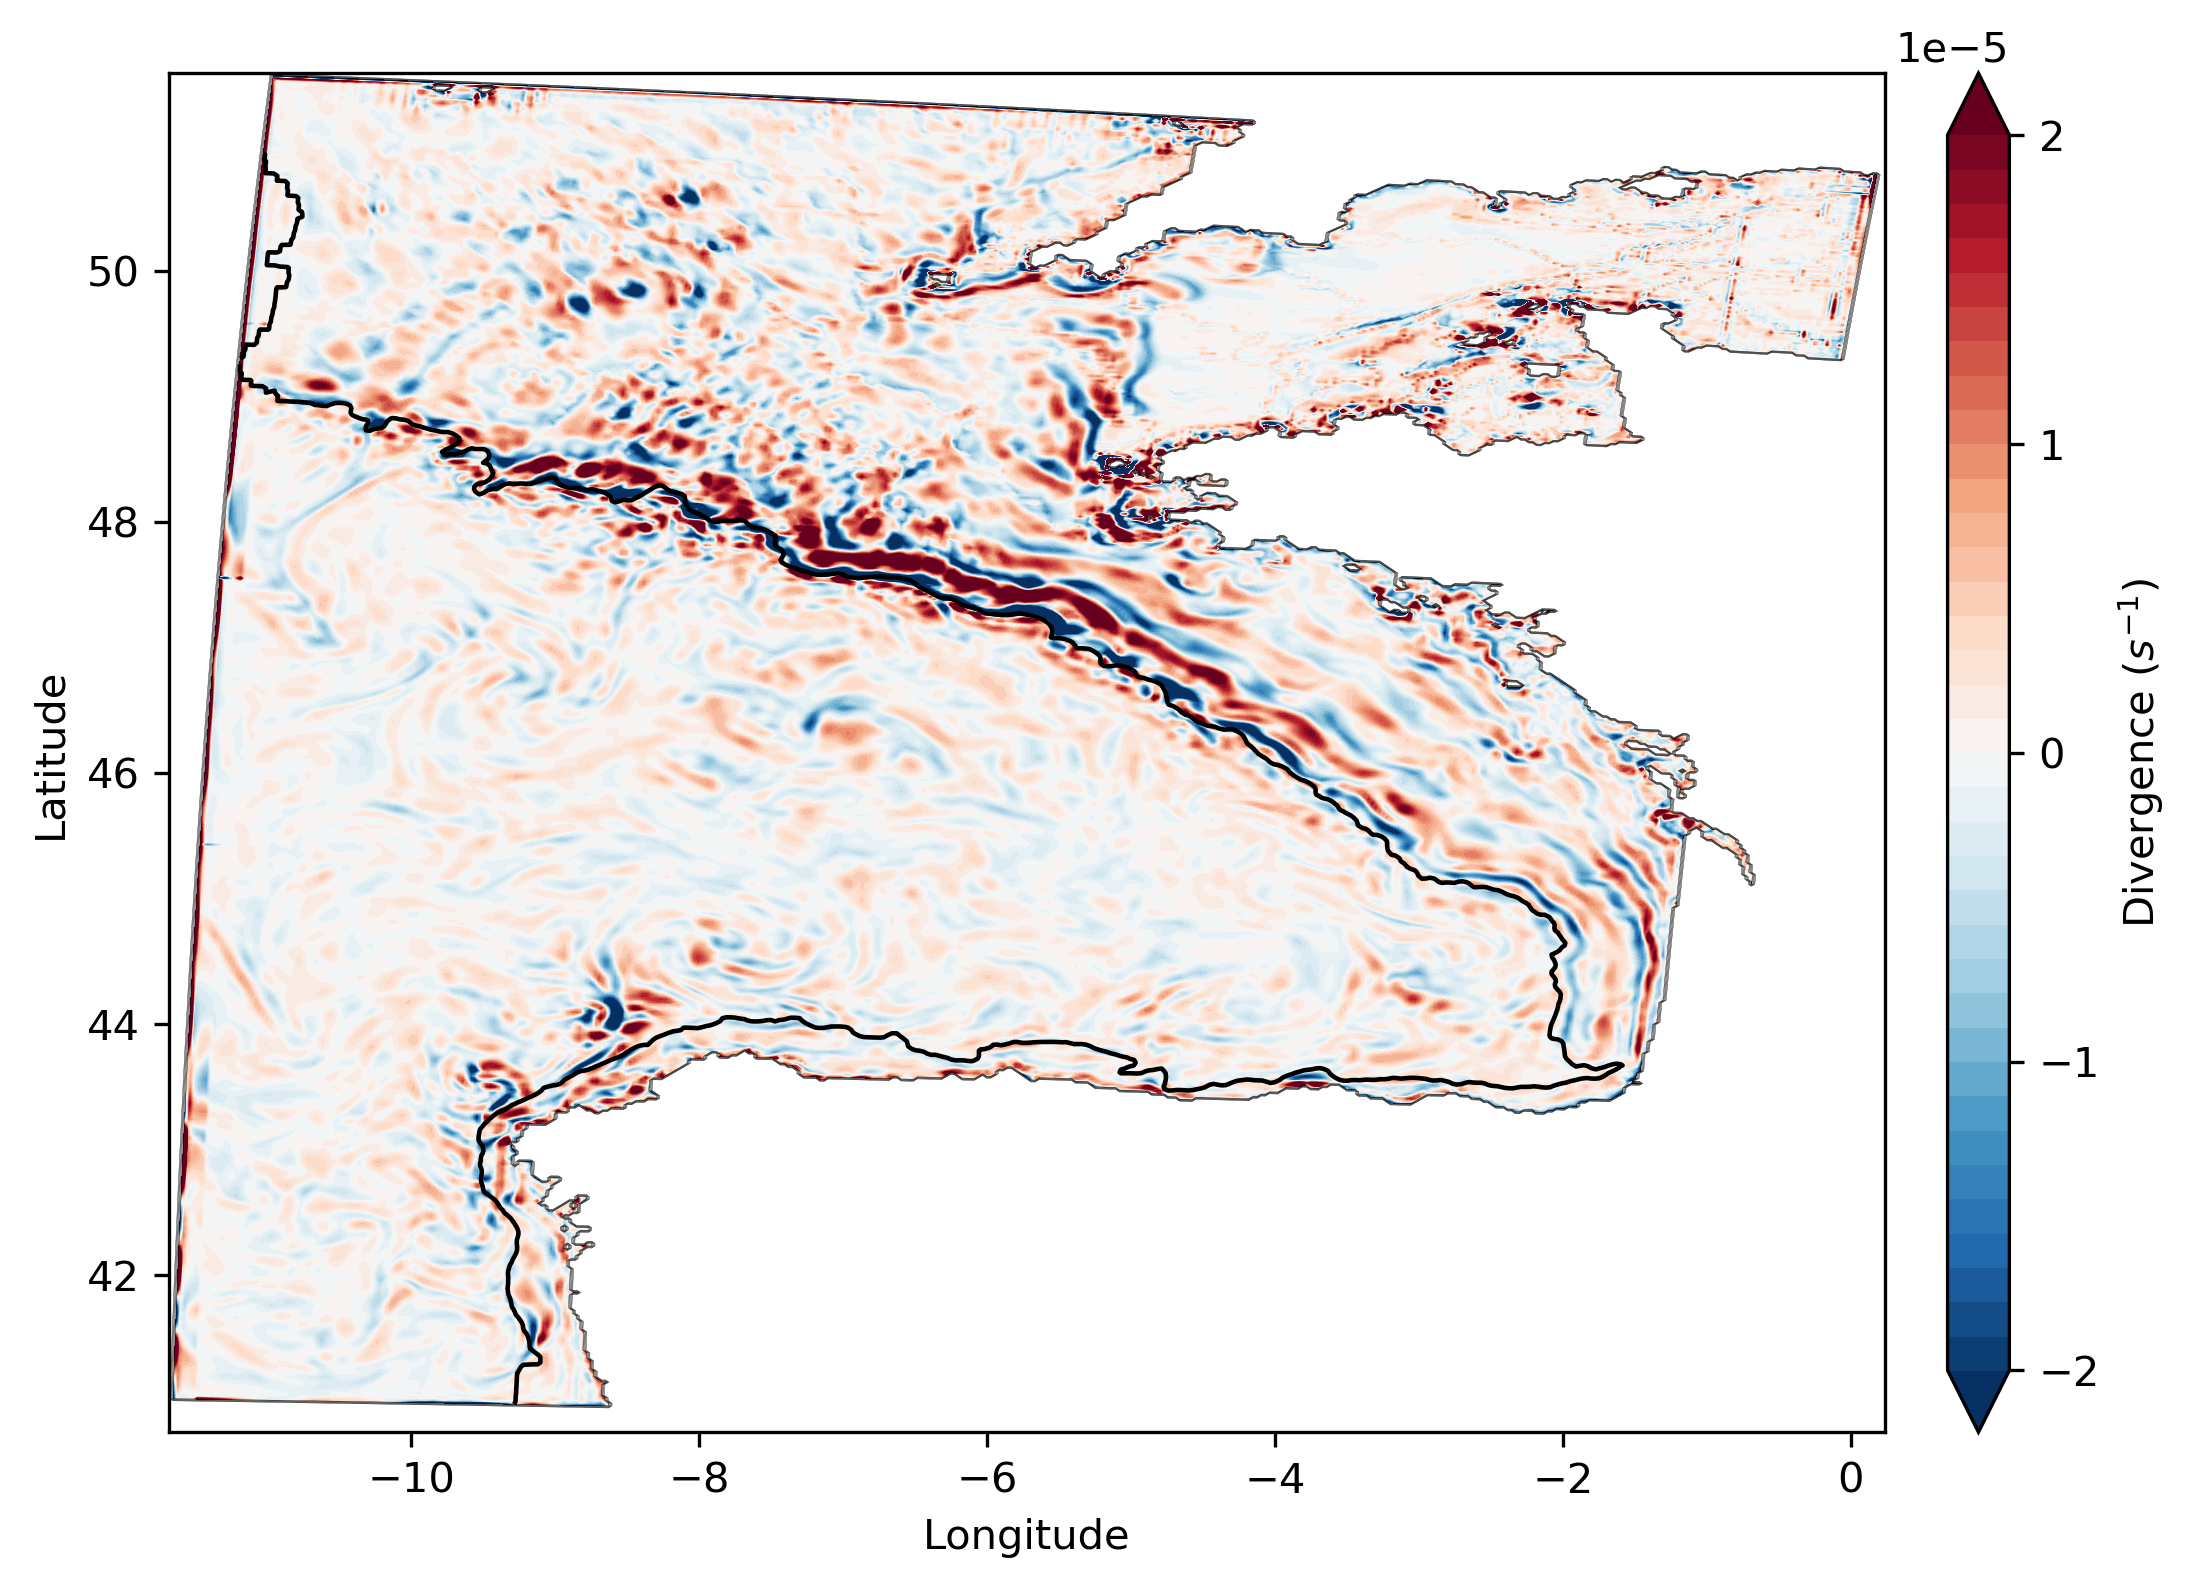
\includegraphics[width=0.8\textwidth]{Definitions/figure8.png}
    \caption{Surface divergence of the horizontal flow ($s^{-1}$) on 28 September 2011 for the TON simulation. The divergence for the TOFF experiment is two orders of magnitude smaller; not shown.}
    \label{fig:divergence}
\end{figure}

%%%%%%%%%%%%%%%%%%%%%%%%%%%%%%%%%%%%%%%%%%
\subsection{Vertical Stratification}
\label{section:3.3}

We calculate the Brunt-V\"ais\"al\"a frequency $N^2$ (Equation~\eqref{eq:bn2}), using the daily modelled profiles of potential temperature and salinity at selected stations depicted in Figure~\ref{fig:bathymetry}, to quantify the impact of tides on the vertical stratification. Figure~\ref{fig:bn2} shows Hovm\"oller plots of the Brunt-V\"ais\"al\"a frequency for the Armorican shelf and the English Channel stations, respectively. The impact of tides on the vertical stratification of the abyssal plain is negligible (except locally near the continental shelf break) and therefore, not shown here for the two simulations.

\begin{figure}[H]
    \centering
    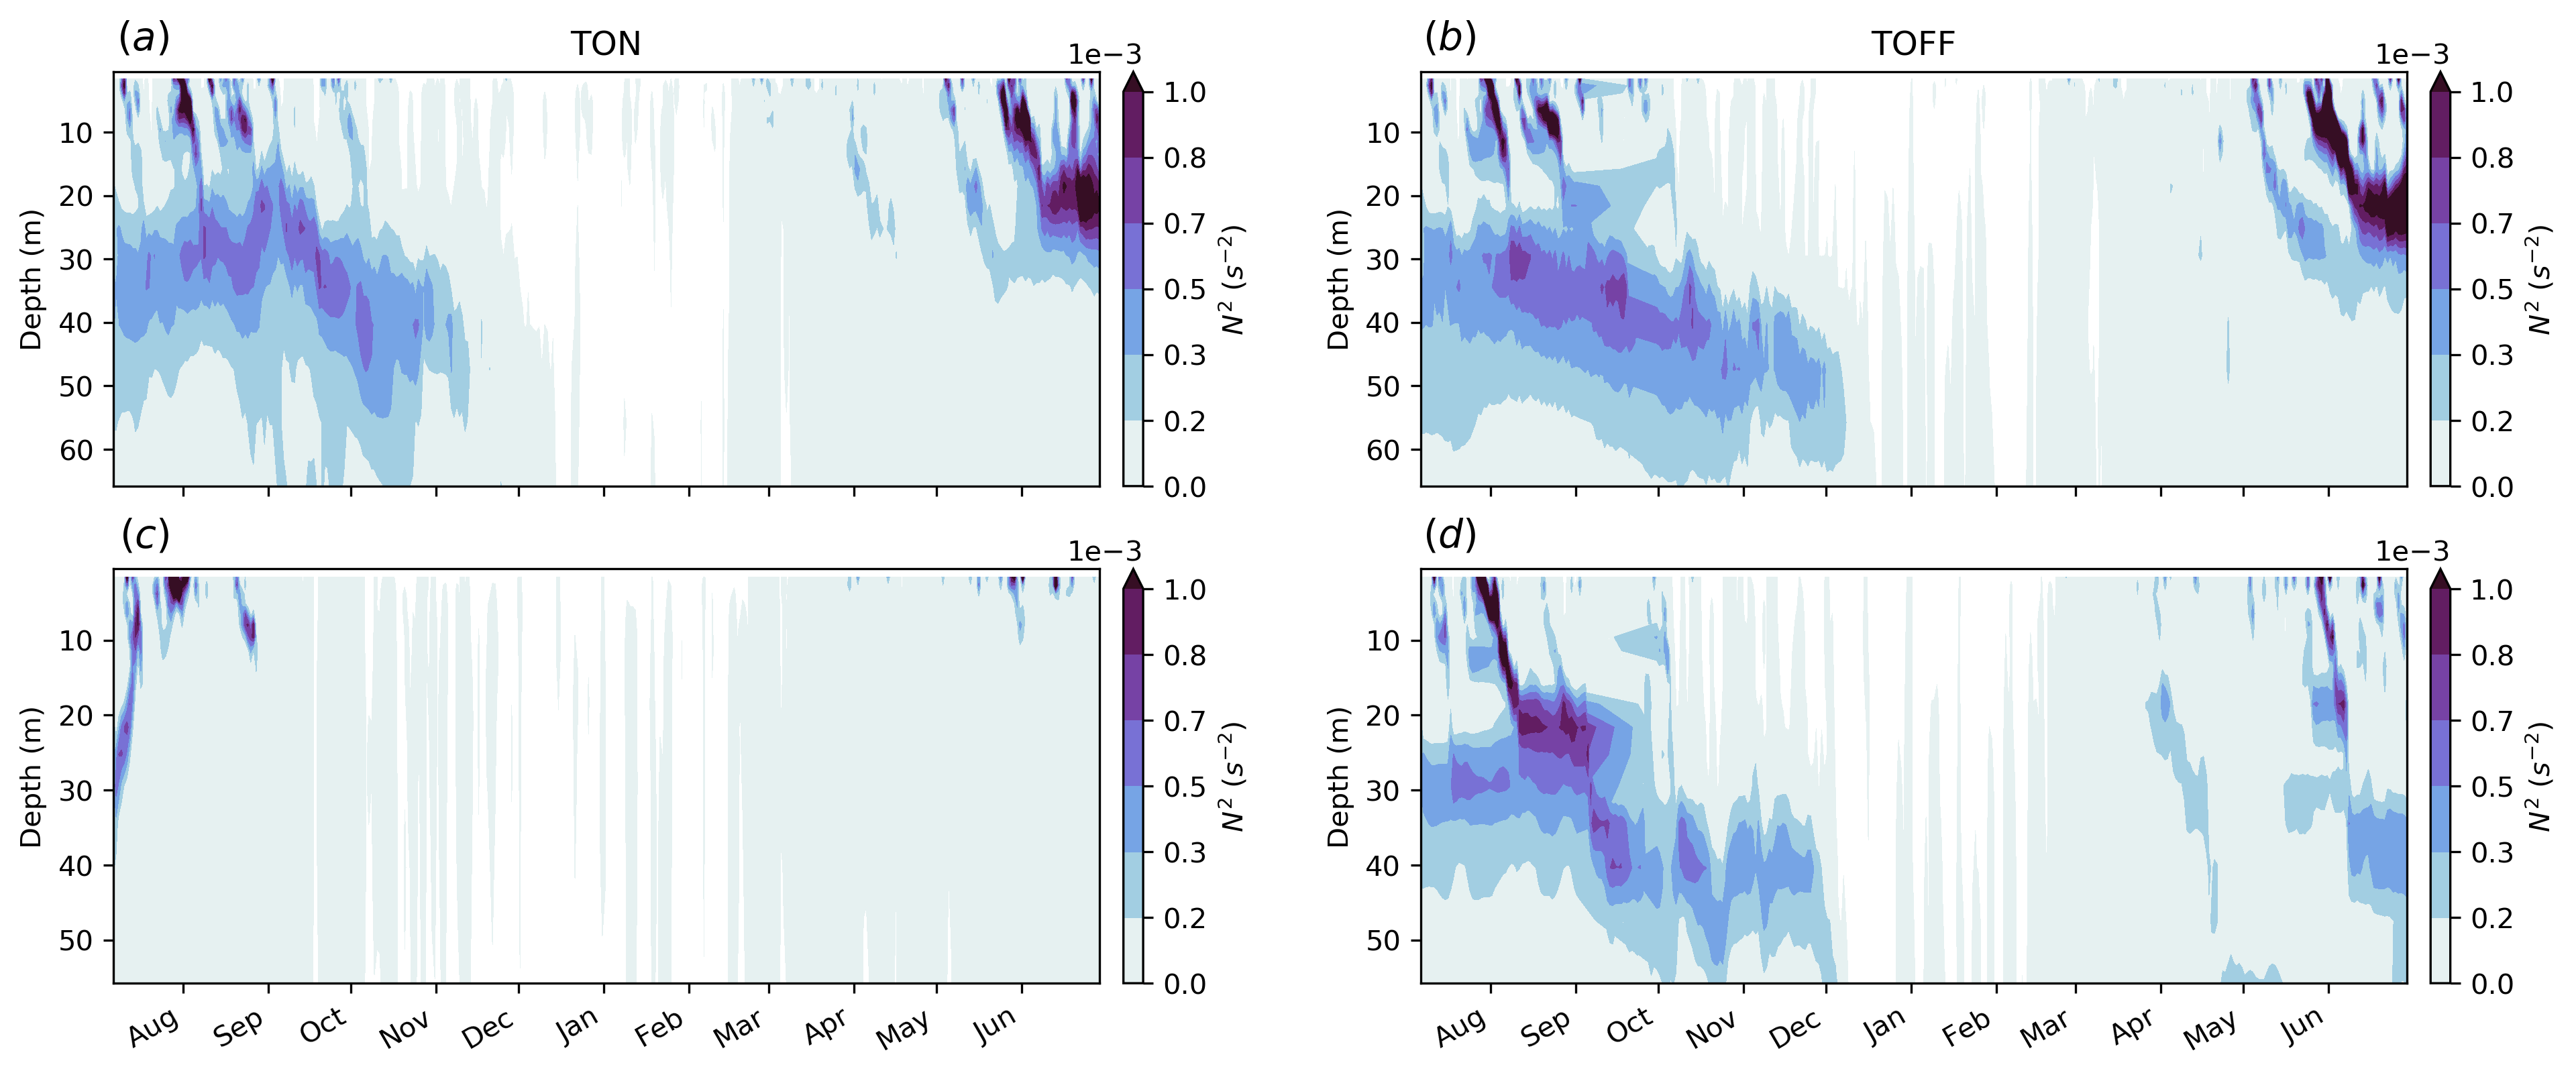
\includegraphics[width=0.8\textwidth]{Definitions/figure9.png}
    \caption{Hovm\"oller plots of the Brunt-V\"ais\"al\"a frequency $(s^{-2})$ calculated for (\textbf{a},\textbf{c}) the TON and (\textbf{b},\textbf{d})~TOFF daily model outputs. The upper panels correspond to the Armorican shelf station and the lower panels to the English Channel station.}
    \label{fig:bn2}
\end{figure}

During winter we observe near-zero values for the Brunt-V\"ais\"al\"a frequency in both simulations, indicating strong mixing due to surface heat loss over the shelves and nearly homogenous conditions in the water column structure (Figure~\ref{fig:bn2}; white areas between December and March). The most prominent differences in the Brunt-V\"ais\"al\"a frequency between the two simulations are observed in summer and during transition periods (i.e.,~spring/fall), when there is a strong stratification due to the thermocline shoaling. The changes brought by tides in the water column are visible in the Armorican shelf at depths below the seasonal thermocline and down to the seabed, and in the English Channel over the whole water column. 

The stratification in the Armorican shelf below the seasonal thermocline, i.e.,~from 20 to 50 m depth, shows high variations and appears to be weaker when tidal forcing is activated, compared with the smoother vertical profiles and the stronger stratification when tides are excluded (Figure~\ref{fig:bn2}a,b). An~interesting remark, is that when tides are activated in the model, the vertical stratification in the English Channel vanishes (almost) completely during the transition periods and in summer, as opposed to the simulation without tides (cf. lack of dark blue colour in Figure~\ref{fig:bn2}c against Figure~\ref{fig:bn2}d).

The mechanism controlling the changes in the vertical stratification over the shelves is associated with the bottom Ekman flow pattern. In the presence of tides, the bottom stress (and its coefficient) is increased, leading to an increase in the vertical velocity shear and mixing in the shelf areas of the English Channel dominated by strong tidal currents. In order to quantify this impact, we calculated the bottom stress when tides were activated and we found an increase by about one order of magnitude larger in the Armorican shelf (i.e.,~values up to 0.1 N/m$^2$) and two orders of magnitude larger in the English Channel (i.e.,~values up to 1 N/m$^2$).
 
%%%%%%%%%%%%%%%%%%%%%%%%%%%%%%%%%%%%%%%%%%
\subsection{Spectral Signatures of Tides}
\label{section:3.4}

In this section, we quantify the impact of high-frequency spatiotemporal tidal signals by means of~frequency and wavenumber energy spectra, using the hourly NEMO model output and examining different regions in the Bay of Biscay.

Figure~\ref{fig:ssh_tseries}a,b shows the hourly modelled SSH variations of the TON and TOFF simulations at~three locations presented in Figure~\ref{fig:bathymetry}. When tides are included, the SSH variations exhibit fortnightly spring-neap consecutive tidal cycles (Figure~\ref{fig:ssh_tseries}a). This is observed in all three areas, with SSH variations being higher in the macrotidal area of the English Channel, followed by the Armorican shelf and the abyssal plain where the smallest variations are observed. When tidal forcing is included in~the simulation, the SSH variations increase by about one order of magnitude in all three locations (Figure~\ref{fig:ssh_tseries}b). We also note that the SSH variations of the TOFF simulation are different from the SSH detided variations in the TON simulation (Figure~\ref{fig:ssh_tseries}c). This is due to the strong interaction between barotropic tides and dynamical processes controlled by mesoscale and small-scale activity, leaving a~residual signal in SSH.


The power spectral density of the SSH hourly variations (Figure~\ref{fig:ssh_tseries}a,b) in the frequency domain is shown in Figure~\ref{fig:ssh_freq}, for both simulations and seasons and the three locations discussed above. The~energy spectra for both seasons present many similarities (Figure~\ref{fig:ssh_freq}a,b), with slightly more energy during winter for the low and semidiurnal frequency bands. Both simulations, with and without tides, have similar energy spectra values at low frequencies (i.e.,~frequencies smaller than 0.4 cpd---cycles per day). The most important differences between the two simulations, are observed for higher frequencies than 0.4 cpd, where energy spectra are significantly decreased, showing a steeper spectral slope, when~tides are not modelled. The energy spectra of the TON simulation (solid lines in Figure~\ref{fig:ssh_freq}a,b) exhibit large peaks at diurnal and semidiurnal frequency bands, at about 1 and 2 cpd, respectively, as a result of the tidal constituents modelled in this simulation. The semidiurnal peaks at 2 cpd appear to have more energy spectra than the diurnal peaks at 1 cpd, in all three locations. This is because the M2 is the main tidal constituent in the Northeastern Atlantic, with large tidal amplitudes (cf. Figure~\ref{fig:tidal_constituents}). In~the high-frequency range (i.e.,~frequencies larger than 3 cpd), smaller peaks are observed including also the M4 tidal constituent at frequencies near the 4 cpd. As expected, in most cases the English Channel (black line in Figure~\ref{fig:ssh_freq}) appears to be the more energetic area compared with the other two areas. For~the higher frequencies, the Armorican shelf (orange line in Figure~\ref{fig:ssh_freq}) appears also to be tidal energetic, especially in periods with strong stratification (Figure~\ref{fig:ssh_freq}a).



\begin{figure}[H]
    \centering
    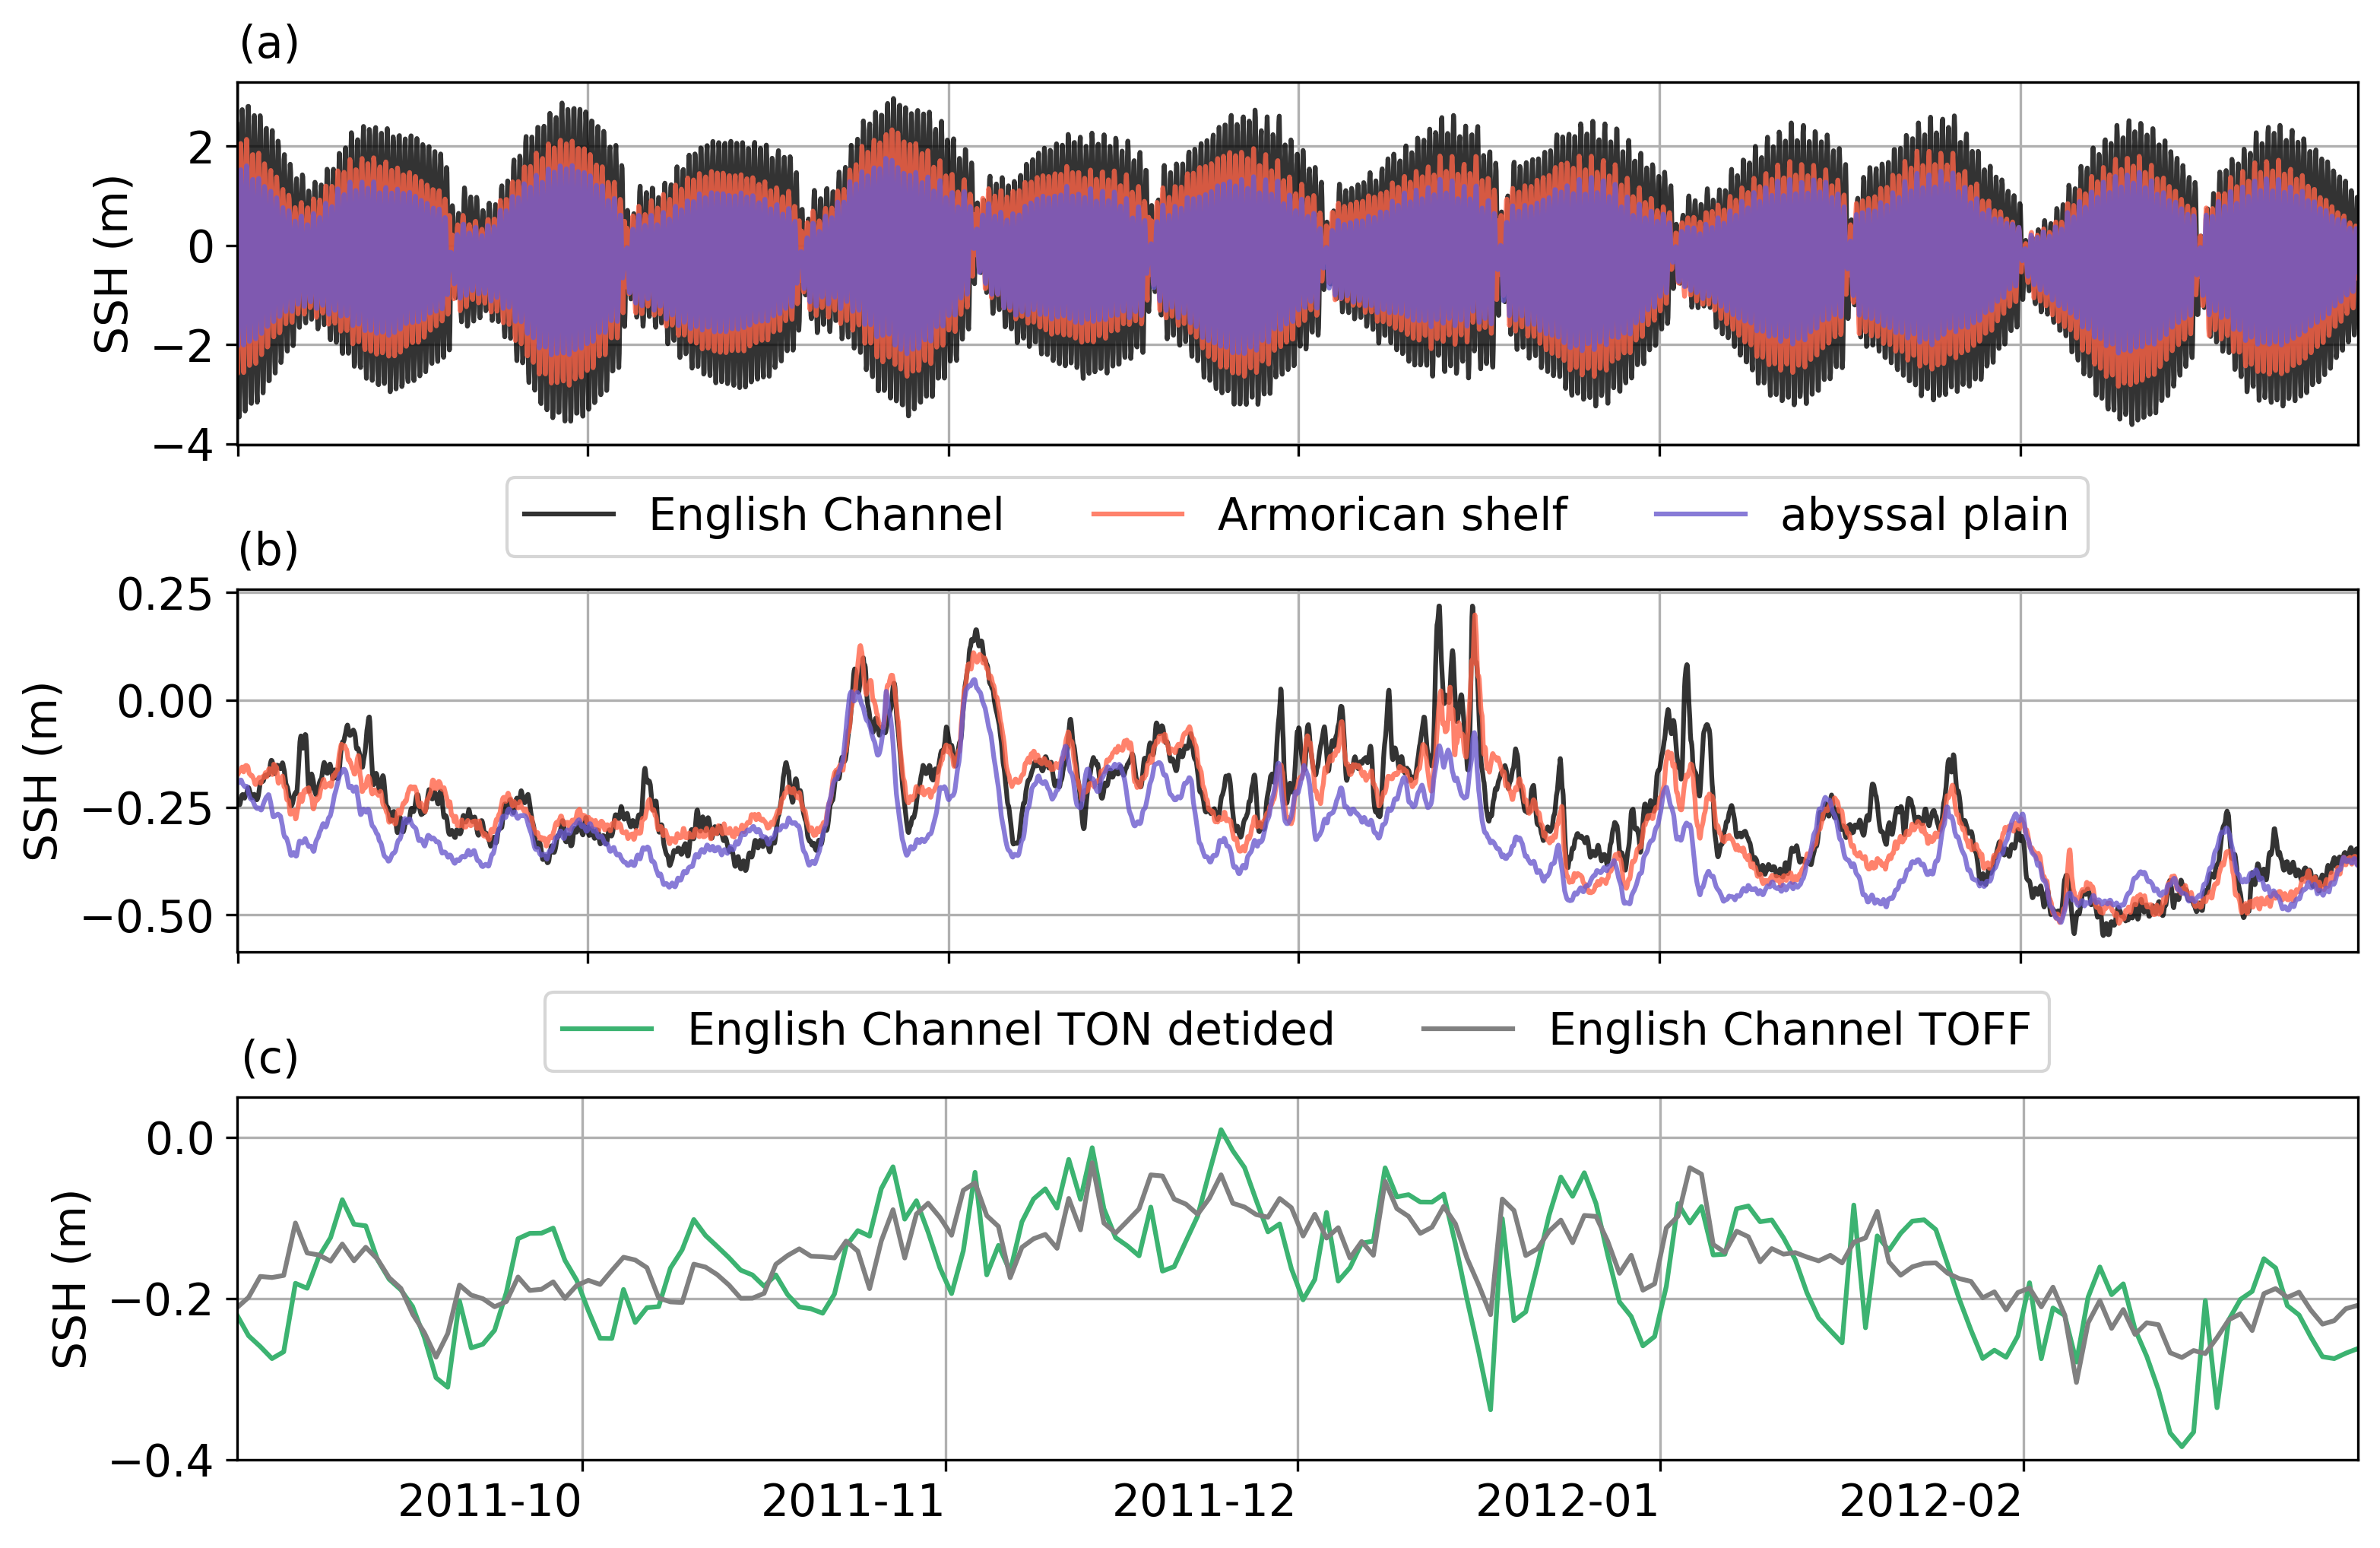
\includegraphics[width=0.8\textwidth]{Definitions/figure10.png}
    \caption{Hourly model variations of SSH in (\textbf{a}) TON and (\textbf{b}) TOFF simulations, for the investigated period from end-summer to mid-winter. The blue line corresponds to the abyssal plain, the red to the Armorican shelf and the black to the English Channel, typical locations showed in Figure~\ref{fig:bathymetry}; (\textbf{c}) daily averaged SSH model variations of the TOFF simulation (grey line) and the detided output results of the TON simulation (green line). The inverse barometer has been removed from the model outputs.} 
    \label{fig:ssh_tseries}
\end{figure}
\unskip
\begin{figure}[H]
    \centering
    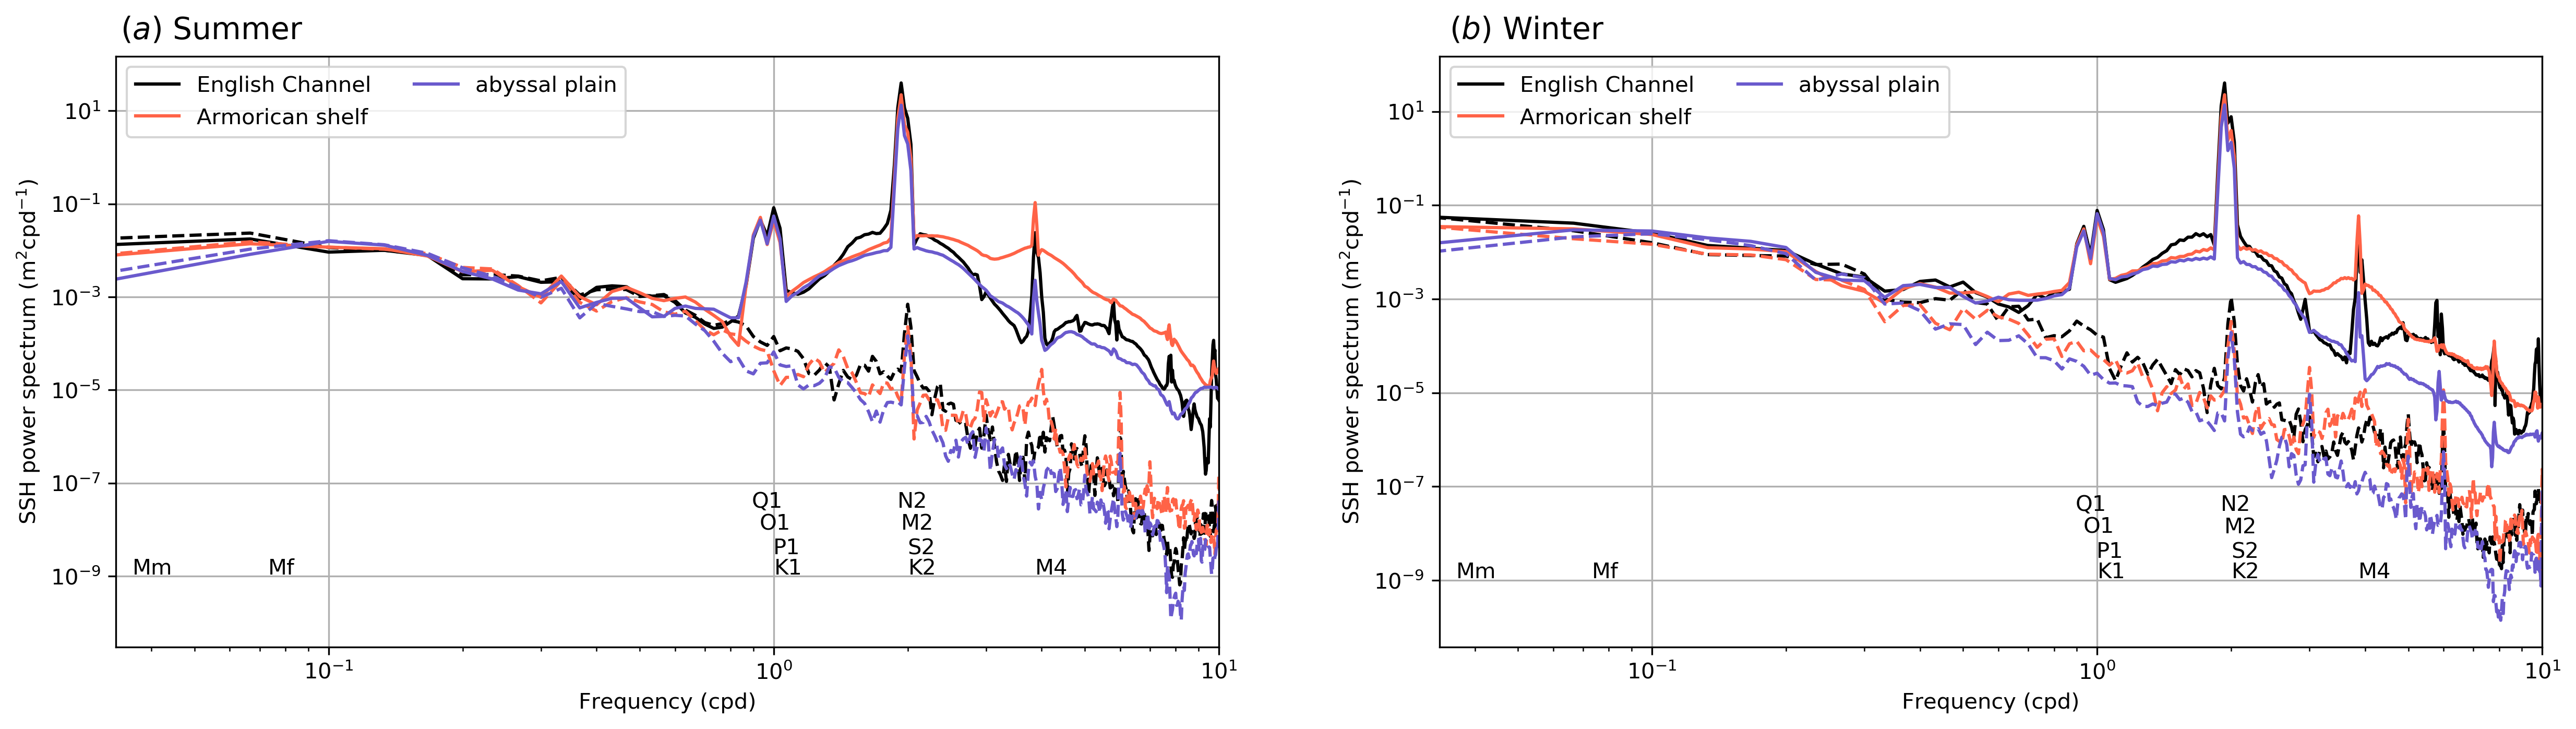
\includegraphics[width=0.95\textwidth]{Definitions/figure11.png}
    \caption{Power spectral density of SSH computed from hourly model outputs on the abyssal plain (blue), the Armorican shelf (red) and the English Channel (black) for (\textbf{a}) summer and (\textbf{b}) winter. Solid~lines correspond to the TON and dashed lines to the TOFF simulation. The modelled tidal constituents are also denoted (from lower to higher frequencies: Mm, Mf, Q1, O1, P1, K1, N2, M2, S2, K2 and M4).} 
    \label{fig:ssh_freq}
\end{figure}

In addition, we investigate the dynamical impact of tides at different spatial scales, performing wavenumber spectral analysis in the abyssal plain (red box area in Figure~\ref{fig:bathymetry}). Figure~\ref{fig:wavenumber_spectra} shows the wavenumber power spectral density computed from hourly SSH and relative vorticity fields, averaged over the summer and winter periods.

\begin{figure}[H]
    \centering
    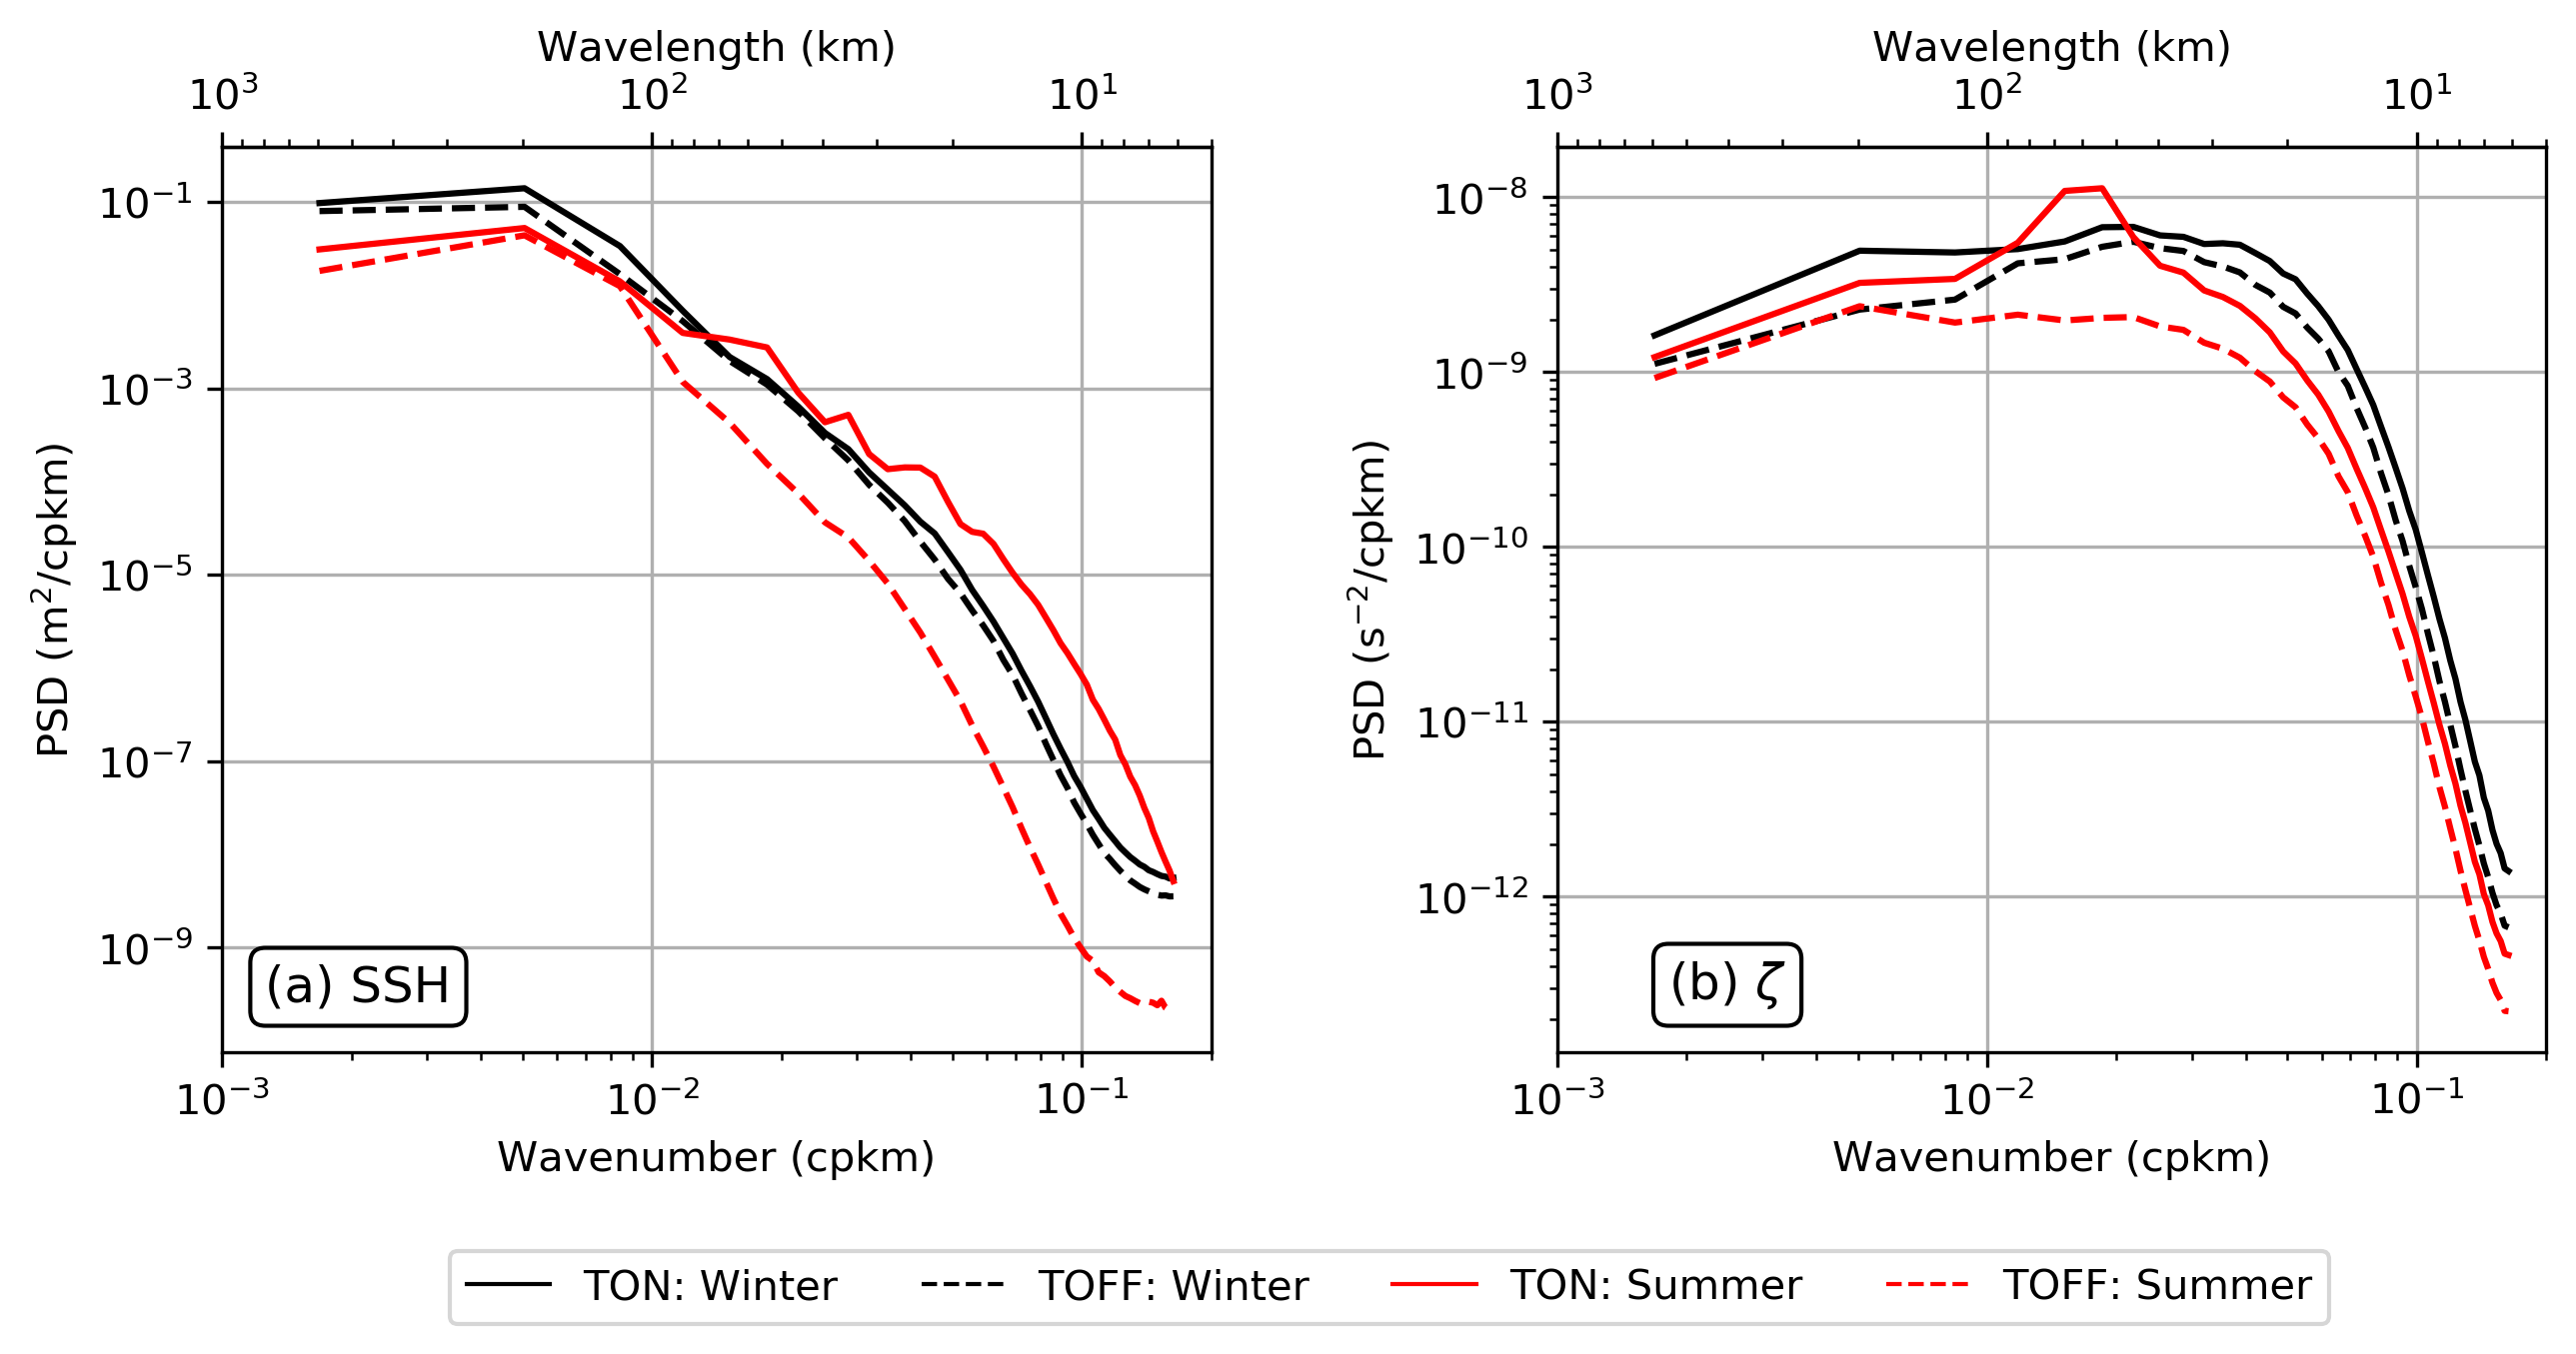
\includegraphics[width=0.8\textwidth]{Definitions/figure12.png}
    \caption{Wavenumber power spectra computed from hourly modelled outputs of (\textbf{a}) SSH and (\textbf{b}) relative vorticity in the spatial area shown in Figure~\ref{fig:bathymetry}, for the TON (solid lines) and TOFF (dashed lines) simulations. Spectra are averaged for the summer (red lines) and winter (black lines) periods.}
    \label{fig:wavenumber_spectra}
\end{figure}

When tides are included, the SSH spectra slope appears to be steeper during winter compared with summer, i.e.,~higher energy values at large-scale and lower energy values at the mesoscale and small-scale (Figure~\ref{fig:wavenumber_spectra}a; solid red/black lines). This is because, during summer when stratification is strong, the tidal forcing appears to contribute energetically on a wider range of spatial scales, from the large to mesoscale and small-scale. When tides are not considered in the simulation, the most prominent spectra differences between the two seasons are observed at the mesoscale and small-scale, by about two orders of magnitudes, with the summer values being the smallest ones (Figure~\ref{fig:wavenumber_spectra}a; dashed red/black lines). The spectral slope during winter when stratification is weak and is not affected by the presence (or not) of tides at the mesoscale and small-scale (Figure~\ref{fig:wavenumber_spectra}a; black solid/dashed lines).

During winter, the relative vorticity spectra appear almost always with more energy compared with its summer values, remaining unchanged by the simulation (or not) of tides (Figure~\ref{fig:wavenumber_spectra}b; red/black lines). The latter remark was also verified by the vorticity maps shown in Figure~\ref{fig:vorticity} and discussed in Section~\ref{section:3.2}. On the other hand, during summer and including tides, there is a marked increase in energy spectra at the mesoscale, with a peak at a range of approximately 70{--}80 km wavelengths (Figure~\ref{fig:wavenumber_spectra}b; solid red line). This finding is explained by the M2 tidal constituent triggering the generation of internal tides and their baroclinic effect on mesoscale activity in the abyssal plain (cf. also~\cite{Pairaud2010}).

%%%%%%%%%%%%%%%%%%%%%%%%%%%%%%%%%%%%%%%%%%
\section{Concluding Remarks}
\label{section:4}

Our results showed that the tidal forcing greatly influences the spatial variability of the SST over the shelves, mostly in shallow macrotidal areas such as the English Channel, and especially in summer and during transition periods when the stratification is strong. At the basin scale, the tidal mixing tends to cool the SSTs during summer, while it tends to increase surface temperatures during winter. The most notable differences were observed locally in the English Channel and especially near the location of the Ushant tidal front, which is only formed when tides are activated in our model simulation. Tides appeared also to impact SSTs by more than $1^\circ$C in the northeastern shelf break area near $47^\circ$ N, where internal tides are generated~\cite{Pairaud2010}. The SST cooling effect of tides was also observed during winter over the Celtic shelf and near the freshwater fronts in the Armorican shelf. 

In the numerical simulation including tides, the surface salinity was increased in the northern part of the Armorican shelf and the English Channel, both in summer and winter. In addition, a reduced river freshwater advection was observed in the cross-shelf area spanning the southeastern part of the Bay of Biscay around  $44^\circ$ N, $3.5^\circ$ W. This result highlights the role of tides on the cross-shelf transport of water masses, between the continental shelf and the deep ocean.

On the continental shelves, the mechanism that triggers the modifications brought by tides is~attributed to the bottom Ekman flow pattern. Our numerical simulations revealed a strong increase of~the bottom stress, subsequently enhancing vertical mixing and weakening stratification in the presence of tides. Our analysis highlights the importance to include in this study an optimal parameterisation of~the bottom stress in areas with strong tidal forcing, greatly influencing model performance in relation to characteristic bathymetric features (e.g.,~continental shelf break) and thermohaline properties (e.g.,~intense frontal activity).

The spectral analysis of SSH revealed a significant imprint on both frequency and wavenumber domains. Frequency spectra showed that tides are contributing in the Bay of Biscay energetics by two to three orders of magnitude, at frequencies higher than 0.4 cpd with large spectral peaks observed near the semidiurnal band at about 2 cpd. Many spectral peaks (consistent also with the frequency of~modelled tidal constituents) were also observed at super-tidal frequency bands, higher than 2 cpd and especially locally in the English Channel, indicating an inherent difficulty of the model to predict the tidal sea level signal. At frequencies lower than 0.4 cpd tides have a negligible impact, despite the fact that the Mm and Mf low-frequency tidal constituents were included in our simulation.

The analysis of SSH wavenumber spectra in the abyssal plain, showed a less steep spectral slope when tides were activated, suggesting a cascade of energy from large (basin) scale to mesoscale and small-scale patterns. This impact of tides to increase the energetics of the mesoscale and small-scale on the expense of large-scale patterns, was more apparent during summer than in winter. An interesting remark for the summer period, when stratification is stronger, is that the vorticity spectral peak was highly increased for mesoscale features with spatial scales at approximately 70--80 km. This is associated with the dynamical impact of internal tides contributing energetically on the mesoscale in the abyssal plain and small-scale on the shelves (cf. also~\cite{Pairaud2010,lelong_kunze_2013}).

The findings of the present study may contribute on our future efforts to improve the representation and parametrisation of tides in ocean models, focusing on their spectral characteristics in a wide range of spatio-temporal scales and their mechanism on the internal tide generation in macrotidal hot spot areas. Finally, our work could also contribute to the calibration and tuning of the sea level tidal signal in ocean modelling frameworks and data products, based on the upcoming wide-swath Surface Water and Ocean Topography (SWOT; \url{https://swot.jpl.nasa.gov/}) satellite altimetry mission.

%%%%%%%%%%%%%%%%%%%%%%%%%%%%%%%%%%%%%%%%%%
% \section{Patents}
% This section is not mandatory, but may be added if there are patents resulting from the work reported in this manuscript.

%%%%%%%%%%%%%%%%%%%%%%%%%%%%%%%%%%%%%%%%%%
\vspace{6pt} 

%%%%%%%%%%%%%%%%%%%%%%%%%%%%%%%%%%%%%%%%%%
\supplementary{The following are available online at \linksupplementary{s1}. The code and plotting scripts used in this analysis are openly available online on GitHub at \url{https://github.com/gkara00/BoB_tides}. The model output files of NEMO are available upon request from the authors.
%
%\begin{figure}[H]
%    \centering
%    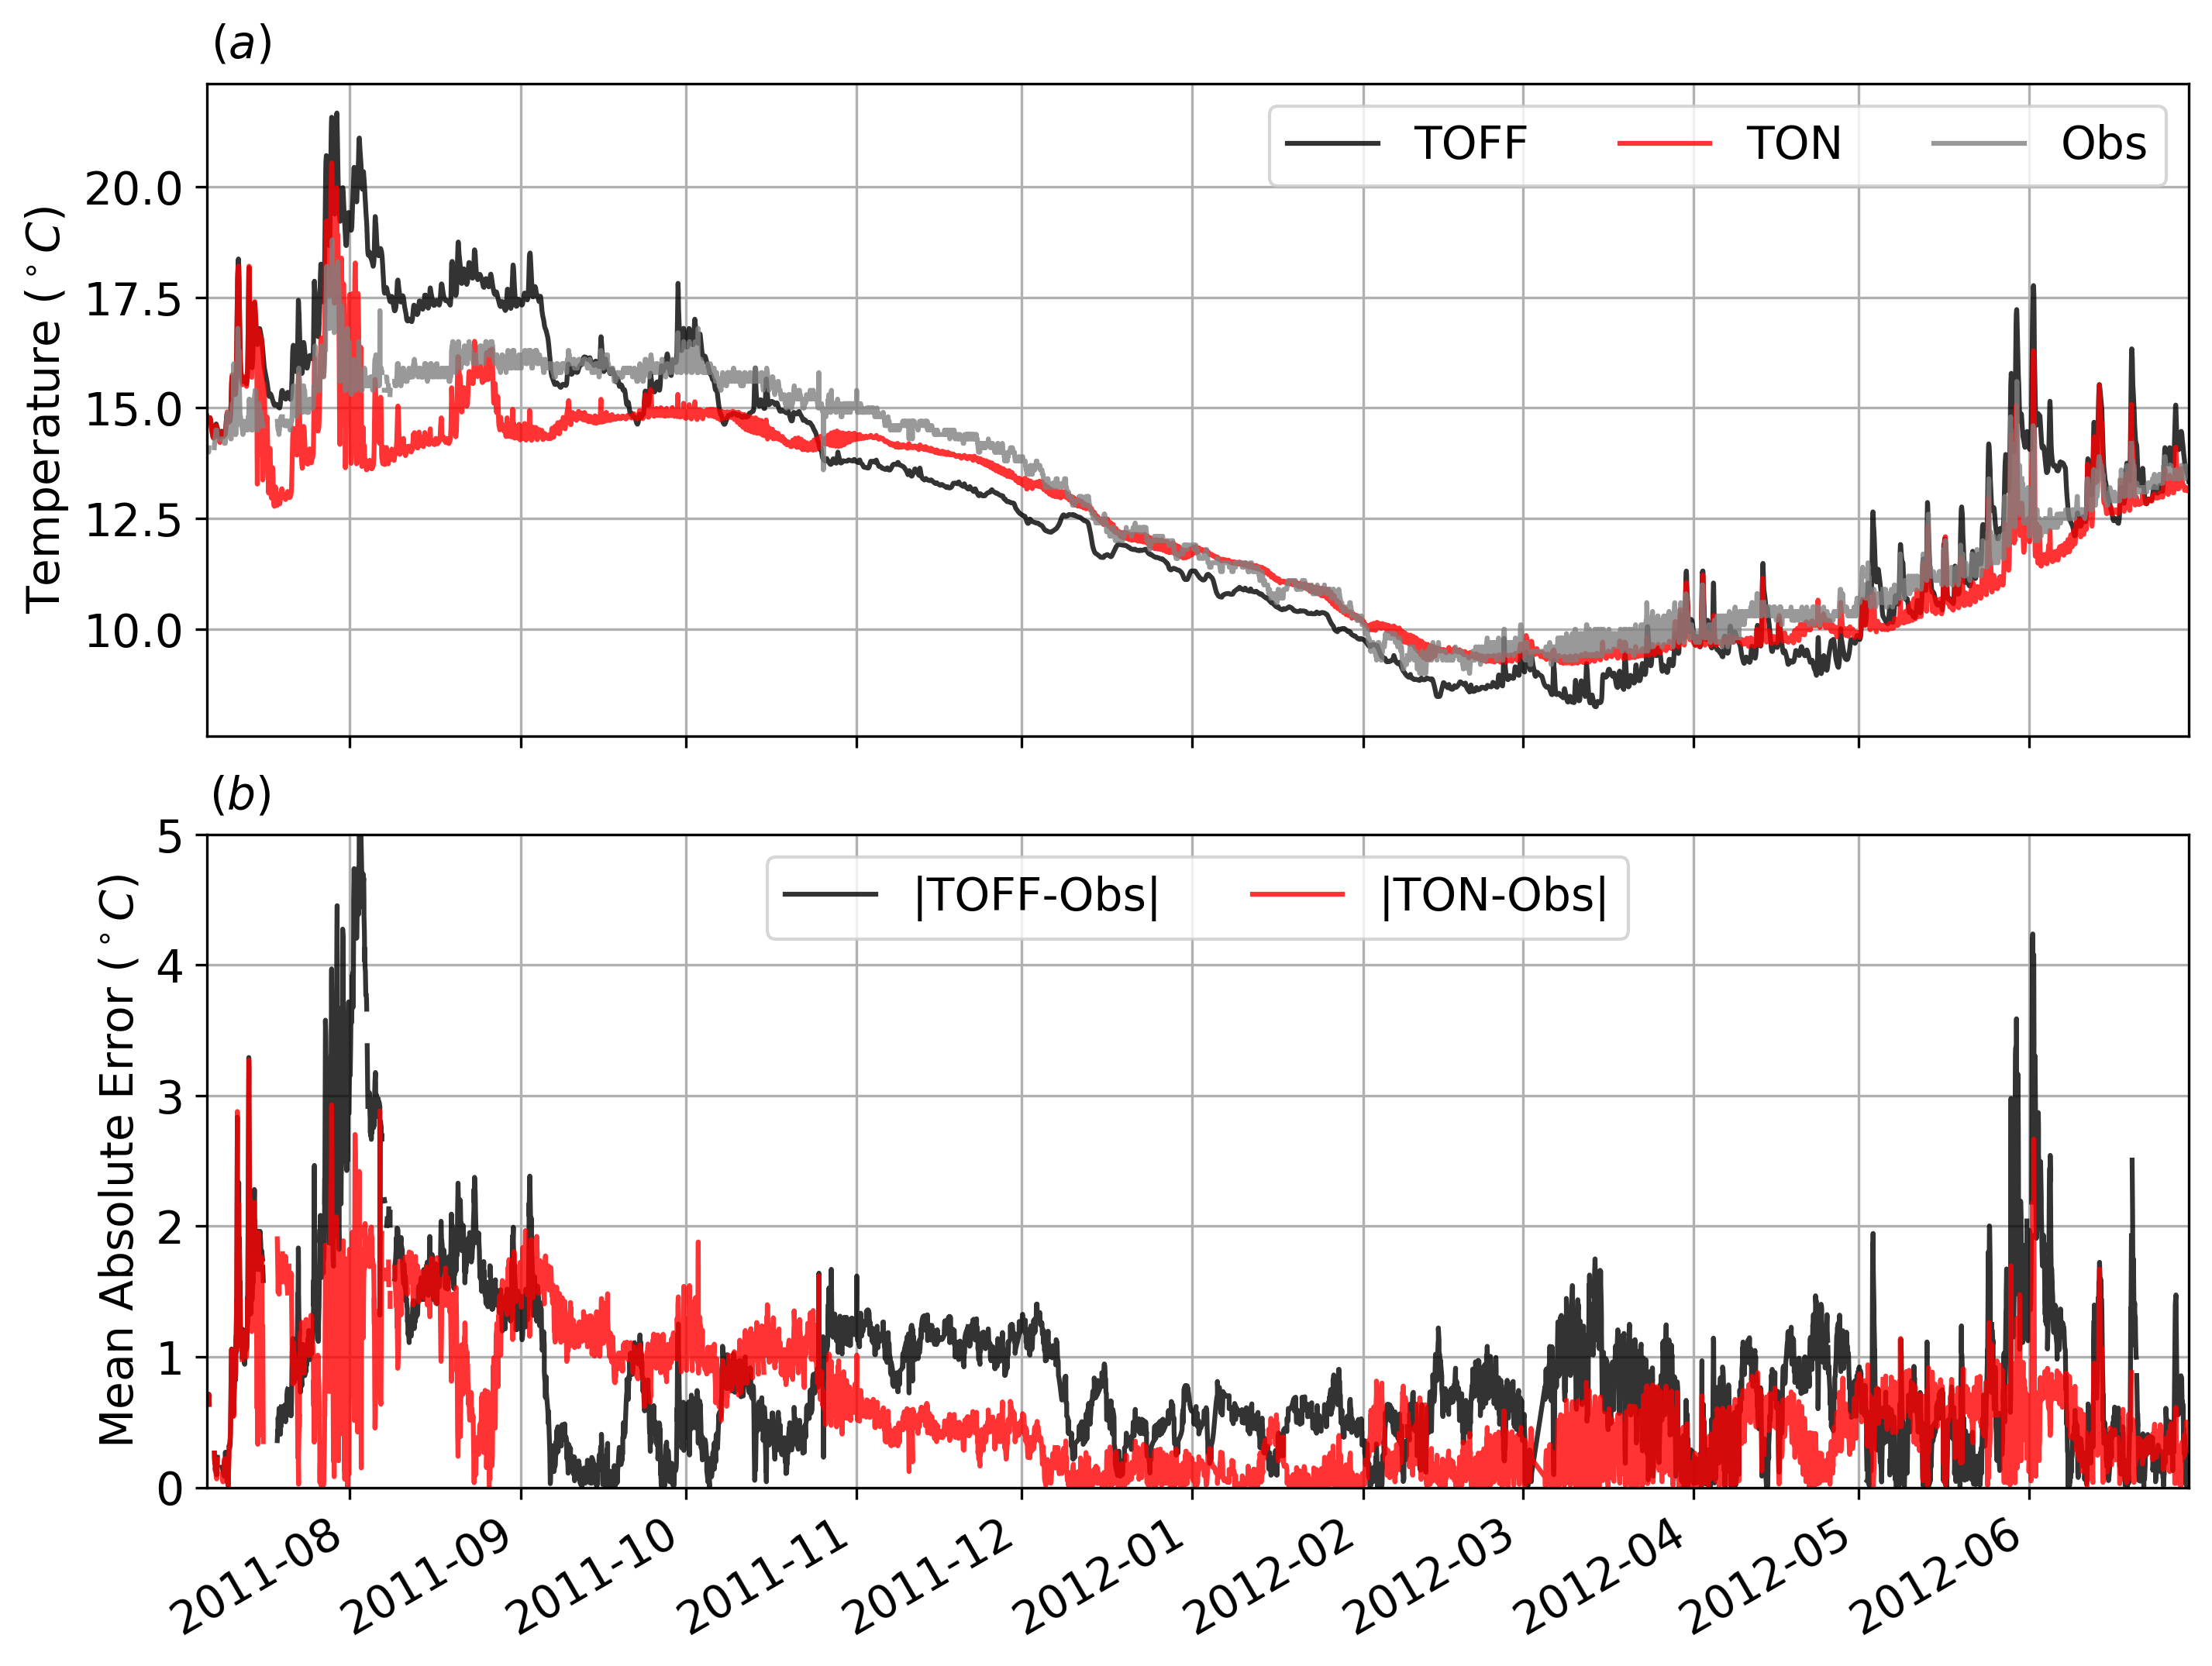
\includegraphics[width=0.95\textwidth]{Definitions/figureS1.png}
%    \caption*{\textbf{Figure S1.} (\textbf{a}) Surface temperature ($^\circ$C) of in-situ data and TON, TOFF model simulations at a station in the English Channel. (\textbf{b}) Mean Absolute Error ($^\circ$C) between model and observations. Station 62103\hl{---}%we changed hyphen to em-dash, please confirm.
%Channel Lightship\hl{---}$49.9^\circ$ N, $2.9^\circ$ W (\url{https://marine.copernicus.eu}).}
%    \label{fig:S1}
%\end{figure}
}

% Only for the journal Methods and Protocols:
% If you wish to submit a video article, please do so with any other supplementary material.
% \supplementary{The following are available at \linksupplementary{s1}, Figure S1: title, Table S1: title, Video S1: title. A supporting video article is available at doi: link.}

%%%%%%%%%%%%%%%%%%%%%%%%%%%%%%%%%%%%%%%%%%
\authorcontributions{Conceptualisation: S.S. and V.V.; methodology: J.K. and V.V.; software: J.K. and V.V.; formal analysis: J.K.; investigation: J.K.; data curation: J.K.; writing{---}%we changed en-dash to em-dash, please confirm.
original draft preparation: J.K.; writing{---}review and editing: V.V. and S.S.; visualisation: J.K.; supervision: S.S. All authors have read and agreed to the published version of the manuscript.}%For research articles with several authors, a short paragraph specifying their individual contributions must be provided. The following statements should be used ``conceptualization, X.X. and Y.Y.; methodology, X.X.; software, X.X.; validation, X.X., Y.Y. and Z.Z.; formal analysis, X.X.; investigation, X.X.; resources, X.X.; data curation, X.X.; writing--original draft preparation, X.X.; writing--review and editing, X.X.; visualization, X.X.; supervision, X.X.; project administration, X.X.; funding acquisition, Y.Y.'', please turn to the  \href{http://img.mdpi.org/data/contributor-role-instruction.pdf}{CRediT taxonomy} for the term explanation. Authorship must be limited to those who have contributed substantially to the work reported.}

%%%%%%%%%%%%%%%%%%%%%%%%%%%%%%%%%%%%%%%%%%
\funding{This research received no external funding}

%%%%%%%%%%%%%%%%%%%%%%%%%%%%%%%%%%%%%%%%%%
\acknowledgments{This work was supported by computational time granted from the Greek Research and Technology Network (GRNET) in the National HPC facility---ARIS---under project ID PA002007. We wish to express our gratitude to Marios Kailas for his technical support in the initial stage of this work and to Panagiotis Andriopoulos for the constructive discussions. We also thank the three anonymous reviewers whose comments greatly improved the manuscript.}

%%%%%%%%%%%%%%%%%%%%%%%%%%%%%%%%%%%%%%%%%%
\conflictsofinterest{The authors declare no conflicts of interest.}%Declare conflicts of interest or state ``The authors declare no conflict of interest.'' Authors must identify and declare any personal circumstances or interest that may be perceived as inappropriately influencing the representation or interpretation of reported research results. Any role of the funders in the design of the study; in the collection, analyses or interpretation of data; in the writing of the manuscript, or in the decision to publish the results must be declared in this section. If there is no role, please state ``The funders had no role in the design of the study; in the collection, analyses, or interpretation of data; in the writing of the manuscript, or in the decision to publish the results''.} 

%%%%%%%%%%%%%%%%%%%%%%%%%%%%%%%%%%%%%%%%%%
%% optional
% \abbreviations{}%The following abbreviations are used in this manuscript:\\

% \noindent 
% \begin{tabular}{@{}ll}
% MDPI & Multidisciplinary Digital Publishing Institute\\
% DOAJ & Directory of open access journals\\
% TLA & Three letter acronym\\
% LD & linear dichroism
% \end{tabular}}

%%%%%%%%%%%%%%%%%%%%%%%%%%%%%%%%%%%%%%%%%%
%% optional
% \appendixtitles{no} %Leave argument "no" if all appendix headings stay EMPTY (then no dot is printed after "Appendix A"). If the appendix sections contain a heading then change the argument to "yes".
% \appendix
% \section{}
% \unskip
% \subsection{}
% The appendix is an optional section that can contain details and data supplemental to the main text. For example, explanations of experimental details that would disrupt the flow of the main text, but nonetheless remain crucial to understanding and reproducing the research shown; figures of replicates for experiments of which representative data is shown in the main text can be added here if brief, or as Supplementary data. Mathematical proofs of results not central to the paper can be added as an appendix.

% \section{}
% All appendix sections must be cited in the main text. In the appendixes, Figures, Tables, etc. should be labeled starting with `A', e.g., Figure A1, Figure A2, etc. 

%%%%%%%%%%%%%%%%%%%%%%%%%%%%%%%%%%%%%%%%%%
% Citations and References in Supplementary files are permitted provided that they also appear in the reference list here. 

%=====================================
% References, variant A: internal bibliography
%=====================================
\reftitle{References}

% The following MDPI journals use author-date citation: Arts, Econometrics, Economies, Genealogy, Humanities, IJFS, JRFM, Laws, Religions, Risks, Social Sciences. For those journals, please follow the formatting guidelines on http://www.mdpi.com/authors/references
% To cite two works by the same author: \citeauthor{ref-journal-1a} (\citeyear{ref-journal-1a}, \citeyear{ref-journal-1b}). This produces: Whittaker (1967, 1975)
% To cite two works by the same author with specific pages: \citeauthor{ref-journal-3a} (\citeyear{ref-journal-3a}, p. 328; \citeyear{ref-journal-3b}, p.475). This produces: Wong (1999, p. 328; 2000, p. 475)

%=====================================
% References, variant B: external bibliography
%=====================================
\begin{thebibliography}{999}
\providecommand{\natexlab}[1]{#1}

\bibitem[Gerkema \em{et~al.}(2004)Gerkema, Lam, and Maas]{Gerkema2004}
Gerkema, T.; Lam, F.P.A.; Maas, L.R.M.
\newblock Internal tides in the Bay of Biscay: Conversion rates and seasonal
effects.
\newblock {\em Deep. Sea Res. Part II Top. Stud. Oceanogr.} {\bf
2004}, {\em 51},~2995--3008.
[\href{http://dx.doi.org/10.1016/j.dsr2.2004.09.012}{CrossRef}]

\bibitem[Guarnieri \em{et~al.}(2013)Guarnieri, Pinardi, Oddo, Bortoluzzi, and
Ravaioli]{Guarnieri2013}
Guarnieri, A.; Pinardi, N.; Oddo, P.; Bortoluzzi, G.; Ravaioli, M.
\newblock Impact of tides in a baroclinic circulation model of the Adriatic
Sea.
\newblock {\em J. Geophys. Res. Ocean.} {\bf 2013}, {\em
118},~166--183.
\newblock
[\href{http://dx.doi.org/10.1029/2012JC007921}{CrossRef}]

\bibitem[Suanda \em{et~al.}(2017)Suanda, Feddersen, and Kumar]{Suanda2017}
Suanda, S.H.; Feddersen, F.; Kumar, N.
\newblock {The Effect of Barotropic and Baroclinic Tides on Coastal
Stratification and Mixing}.
\newblock {\em J. Geophys. Res. Ocean.} {\bf 2017}, {\em
122},~10156--10173.
\newblock
[\href{http://dx.doi.org/10.1002/2017JC013379}{CrossRef}]

\bibitem[Stanev and Ricker(2020)]{Stanev2020}
Stanev, E.V.; Ricker, M.
\newblock {Interactions between barotropic tides and mesoscale processes in
deep ocean and shelf regions}.
\newblock {\em Ocean. Dyn.} {\bf 2020}, {\em 70},~713--728.
\newblock
[\href{http://dx.doi.org/10.1007/s10236-020-01348-6}{CrossRef}]

\bibitem[Holt \em{et~al.}(2017)Holt, Hyder, Ashworth, Harle, Hewitt, Liu, New,
Pickles, Porter, Popova, Allen, Siddorn, and Wood]{Holt2017}
Holt, J.; Hyder, P.; Ashworth, M.; Harle, J.; Hewitt, H.T.; Liu, H.; New, A.L.;
Pickles, S.; Porter, A.; Popova,~E.;~et al.
\newblock Prospects for improving the representation of coastal and shelf seas
in global ocean models.
\newblock {\em Geosci. Model Dev.} {\bf 2017}, {\em 10},~499--523.
\newblock
[\href{http://dx.doi.org/10.5194/gmd-10-499-2017}{CrossRef}]

\bibitem[Stammer \em{et~al.}(2014)Stammer, Ray, Andersen, Arbic, Bosch,
Carr{\'{e}}re, Cheng, Chinn, Dushaw, Egbert, Erofeeva, Fok, Green, Griffiths,
King, Lapin, Lemoine, Luthcke, Lyard, Morison, Müller, Padman, Richman,
Shriver, Shum, Taguchi, and Yi]{stammer2014}
Stammer, D.; Ray, R.D.; Andersen, O.B.; Arbic, B.K.; Bosch, W.; Carr{\'{e}}re,
L.; Cheng, Y.; Chinn, D.S.; Dushaw,~B.D.; Egbert, G.D.; et al.
\newblock Accuracy assessment of global barotropic ocean tide models.
\newblock {\em Rev.~Geophys.} {\bf 2014},~{\em 52},~243--282.
\newblock
[\href{http://dx.doi.org/10.1002/2014RG000450}{CrossRef}]

\bibitem[Koutsikopoulos and {Le Cann}(1996)]{koutsikopoulos1996}
Koutsikopoulos, C.; {Le Cann}, B.
\newblock {Physical processes and hydrological structures related to the Bay of
Biscay anchovy}.
\newblock {\em Sci. Mar.} {\bf 1996}, {\em 60},~9--19.

\bibitem[{Le Cann}(1990)]{LECANN1990}
{Le Cann}, B.
\newblock Barotropic tidal dynamics of the Bay of Biscay shelf: Observations,
numerical modelling and physical interpretation.
\newblock {\em Cont. Shelf Res.} {\bf 1990}, {\em 10},~723--758.
\newblock
 [\href{http://dx.doi.org/10.1016/0278-4343(90)90008-A}{CrossRef}]

\bibitem[Pairaud \em{et~al.}(2008)Pairaud, Lyard, Auclair, Letellier, and
Marsaleix]{Pairaud2008}
Pairaud, I.L.; Lyard, F.; Auclair, F.; Letellier, T.; Marsaleix, P.
\newblock {Dynamics of the semi-diurnal and quarter-diurnal internal tides in
the Bay of Biscay. Part 1: Barotropic tides}.
\newblock {\em Cont. Shelf Res.} {\bf 2008}, {\em 28},~1294--1315.
\newblock
 [\href{http://dx.doi.org/10.1016/j.csr.2008.03.004}{CrossRef}]

\bibitem[Pingree and {Le Cann}(1990)]{pingree_lc1990}
Pingree, R.D.; {Le Cann}, B.
\newblock Structure, strength and seasonality of the slope currents in the Bay
of Biscay region.
\newblock {\em J. Mar. Biol. Assoc. UK} {\bf 1990}, {\em 70},~857–885.
\newblock
[\href{http://dx.doi.org/10.1017/S0025315400059117}{CrossRef}]

\bibitem[Garcia-Soto \em{et~al.}(2002)Garcia-Soto, Pingree, and
Vald\'es]{Garcia-Soto2002}
Garcia-Soto, C.; Pingree, R.D.; Vald\'es, L.
\newblock {Navidad development in the southern Bay of Biscay: Climate change
and swoddy structure from remote sensing and in situ measurements}.
\newblock {\em J. Geophys. Res.} {\bf 2002}, {\em 107},~3118.
\newblock
[\href{http://dx.doi.org/10.1029/2001JC001012}{CrossRef}]

\bibitem[{Le Boyer} \em{et~al.}(2009){Le Boyer}, Cambon, Daniault, Herbette,
{Le Cann}, Marié, and Morin]{LEBOYER2009}
{Le Boyer}, A.; Cambon, G.; Daniault, N.; Herbette, S.; {Le Cann}, B.; Marié,
L.; Morin, P.
\newblock Observations of the Ushant tidal front in September 2007.
\newblock {\em Cont. Shelf Res.} {\bf 2009}, {\em 29},~1026--1037.
 [\href{http://dx.doi.org/10.1016/j.csr.2008.12.020}{CrossRef}]

\bibitem[Pingree and {Le Cann}(1992{\natexlab{a}})]{pingree1992a}
Pingree, R.D.; {Le Cann}, B.
\newblock Anticyclonic eddy X91 in the southern Bay of Biscay, May 1991 to
February 1992.
\newblock {\em J. Geophys. Res. Ocean.} {\bf 1992}, {\em
97},~14353--14367.
\newblock
[\href{http://dx.doi.org/10.1029/92JC01181}{CrossRef}]

\bibitem[Pingree and {Le Cann}(1992{\natexlab{b}})]{pingree1992b}
\textls[-25]{Pingree, R.D.; {Le Cann}, B.
\newblock {Three anticyclonic slope water oceanic eDDIES (SWODDIES) in the
Southern Bay of Biscay in 1990}.
\newblock {\em Deep. Sea Res. Part Oceanogr. Res. Pap.} {\bf
1992}, {\em 39},~1147--1175.}
\newblock
 [\href{http://dx.doi.org/10.1016/0198-0149(92)90062-X}{CrossRef}]

\bibitem[Reverdin \em{et~al.}(2013)Reverdin, Marié, Lazure, d'Ovidio, Boutin,
Testor, Martin, Lourenco, Gaillard, Lavin, Rodriguez, Somavilla, Mader,
Rubio, Blouch, Rolland, Bozec, Charria, Batifoulier, Dumas, Louazel, and
Chanut]{REVERDIN2013}
Reverdin, G.; Marié, L.; Lazure, P.; d'Ovidio, F.; Boutin, J.; Testor, P.;
Martin, N.; Lourenco, A.; Gaillard, F.; Lavin, A.; et al.
\newblock Freshwater from the Bay of Biscay shelves in 2009.
\newblock {\em J. Mar. Syst.} {\bf 2013}, {\em {109--110}%please add correct volume.
},~S134--S143.
[\href{http://dx.doi.org/10.1016/j.jmarsys.2011.09.017}{CrossRef}]

\bibitem[Porter \em{et~al.}(2016)Porter, Inall, Green, Simpson, Dale, and
Miller]{PORTER2016}
Porter, M.; Inall, M.E.; Green, J.A.M.; Simpson, J.H.; Dale, A.C.; Miller, P.I.
\newblock Drifter observations in the summer time Bay of Biscay slope current.
\newblock {\em J. Mar. Syst.} {\bf 2016}, {\em 157},~65--74.
\newblock
[\href{http://dx.doi.org/10.1016/j.jmarsys.2016.01.002}{CrossRef}]

\bibitem[Rubio \em{et~al.}(2018)Rubio, Caballero, Orfila, Hernández-Carrasco,
Ferrer, Gonz{\'{a}}lez, Solabarrieta, and Mader]{RUBIO2018}
Rubio, A.; Caballero, A.; Orfila, A.; Hernández-Carrasco, I.; Ferrer, L.;
Gonz{\'{a}}lez, M.; Solabarrieta, L.; Mader,~J.
\newblock Eddy-induced cross-shelf export of high Chl-a coastal waters in the
SE Bay of Biscay.
\newblock {\em Remote. Sens. Environ.} {\bf 2018}, {\em 205},~290--304.
\newblock
 [\href{http://dx.doi.org/10.1016/j.rse.2017.10.037}{CrossRef}]

\bibitem[Akpınar \em{et~al.}(2020)Akpınar, Charria, Theetten, and
Vandermeirsch]{Akpnar2020}
Akpınar, A.; Charria, G.; Theetten, S.; Vandermeirsch, F.
\newblock {Cross-shelf exchanges in the northern Bay of Biscay}.
\newblock {\em J. Mar. Syst.} {\bf 2020}, {\em 205}.
\newblock
[\href{http://dx.doi.org/10.1016/j.jmarsys.2020.103314}{CrossRef}]

\bibitem[Baines(1982)]{BAINES1982}
Baines, P.G.
\newblock On internal tide generation models.
\newblock {\em Deep. Sea Res. Part A Oceanogr. Res. Pap.} {\bf
1982}, {\em 29},~307--338.
\newblock
[\href{http://dx.doi.org/10.1016/0198-0149(82)90098-X}{CrossRef}]

\bibitem[Pingree \em{et~al.}(1986)Pingree, Mardell, and New]{Pingree1986}
Pingree, R.D.; Mardell, G.T.; New, A.L.
\newblock {Propagation of internal tides from the upper slopes of the Bay of
Biscay}.
\newblock {\em Nature} {\bf 1986}, {\em 321},~154--158.
\newblock
[\href{http://dx.doi.org/10.1038/321154a0}{CrossRef}]

\bibitem[Pingree and New(1995)]{PINGREE1995}
Pingree, R.D.; New, A.L.
\newblock Structure, seasonal development and sunglint spatial coherence of the
internal tide on the Celtic and Armorican shelves and in the Bay of Biscay.
\newblock {\em Deep. Sea Res. Part I Oceanogr. Res. Pap.} {\bf
1995},~{\em 42},~245--284.
\newblock
 [\href{http://dx.doi.org/10.1016/0967-0637(94)00041-P}{CrossRef}]

\bibitem[Pichon and Correard(2006)]{Pichon2006}
Pichon, A.; Correard, S.
\newblock {Internal tides modelling in the Bay of Biscay. Comparisons with
observations}.
\newblock {\em Sci.~Mar.} {\bf 2006}, {\em 70},~65--88.
\newblock
 [\href{http://dx.doi.org/10.3989/scimar.2006.70s165}{CrossRef}]

\bibitem[Pairaud \em{et~al.}(2010)Pairaud, Auclair, Marsaleix, Lyard, and
Pichon]{Pairaud2010}
Pairaud, I.L.; Auclair, F.; Marsaleix, P.; Lyard, F.; Pichon, A.
\newblock {Dynamics of the semi-diurnal and quarter-diurnal internal tides in
the Bay of Biscay. Part 2: Baroclinic tides}.
\newblock {\em Cont. Shelf Res.} {\bf 2010}, {\em 30},~253--269.
\newblock
 [\href{http://dx.doi.org/10.1016/j.csr.2009.10.008}{CrossRef}]

\bibitem[Egbert and Ray(2003)]{Egbert2003}
Egbert, G.D.; Ray, R.D.
\newblock Semi-diurnal and diurnal tidal dissipation from TOPEX/Poseidon
altimetry.
\newblock {\em Geophys.~Res.~Lett.} {\bf 2003}, {\em 30, 17
}.
\newblock
 [\href{http://dx.doi.org/10.1029/2003GL017676}{CrossRef}]

\bibitem[Pasquet \em{et~al.}(2012)Pasquet, Szekely, and Morel]{PASQUET2012}
Pasquet, A.; Szekely, T.; Morel, Y.
\newblock Production and dispersion of mixed waters in stratified coastal
areas.
\newblock {\em Cont.~Shelf~Res.} {\bf 2012}, {\em 39-40},~49--77.
\newblock
 [\href{http://dx.doi.org/10.1016/j.csr.2012.04.001}{CrossRef}]

\bibitem[Chevallier \em{et~al.}(2014)Chevallier, Herbette, Mari{\'{e}}, {Le
Borgne}, Marsouin, P{\'{e}}r{\'{e}}, Levier, and Reason]{CHEVALLIER2014}
Chevallier, C.; Herbette, S.; Mari{\'{e}}, L.; {Le Borgne}, P.; Marsouin, A.;
P{\'{e}}r{\'{e}}, S.; Levier, B.; Reason, C.
\newblock Observations of the Ushant front displacements with MSG/SEVIRI
derived sea surface temperature data.
\newblock {\em Remote.~Sens.~Environ.} {\bf 2014}, {\em 146},~3--10.
 [\href{http://dx.doi.org/10.1016/j.rse.2013.07.038}{CrossRef}]

\bibitem[Schultes \em{et~al.}(2013)Schultes, Sourisseau, {Le Masson}, Lunven,
and Marié]{SCHULTES2013}
Schultes, S.; Sourisseau, M.; {Le Masson}, E.; Lunven, M.; Marié, L.
\newblock Influence of physical forcing on mesozooplankton communities at the
Ushant tidal front.
\newblock {\em J. Mar. Syst.} {\bf 2013}, {\em {109--110}},~S191--S202.
 [\href{http://dx.doi.org/10.1016/j.jmarsys.2011.11.025}{CrossRef}]

\bibitem[Simpson and Bowers(1981)]{simpson1981}
Simpson, J.; Bowers, D.
\newblock Models of stratification and frontal movement in shelf seas.
\newblock {\em Deep. Sea Res. Part A Oceanogr. Res. Pap.} {\bf
1981}, {\em 28},~727--738.
\newblock
 [\href{http://dx.doi.org/10.1016/0198-0149(81)90132-1}{CrossRef}]

\bibitem[Bowers and Simpson(1987)]{bowerS1987}
Bowers, D.; Simpson, J.
\newblock Mean position of tidal fronts in European-shelf seas.
\newblock {\em Cont. Shelf Res.} {\bf 1987}, {\em 7},~35--44.
\newblock
 [\href{http://dx.doi.org/10.1016/0278-4343(87)90062-8}{CrossRef}]

\bibitem[Holt and Umlauf(2008)]{holt2008}
Holt, J.; Umlauf, L.
\newblock Modelling the tidal mixing fronts and seasonal stratification of the
Northwest European Continental shelf.
\newblock {\em Cont. Shelf Res.} {\bf 2008}, {\em 28},~887--903.
\newblock
 [\href{http://dx.doi.org/10.1016/j.csr.2008.01.012}{CrossRef}]

\bibitem[O’Dea \em{et~al.}(2012)O’Dea, Arnold, Edwards, Furner, Hyder,
Martin, Siddorn, Storkey, While, Holt, and Liu]{odea2012}
O’Dea, E.J.; Arnold, A.K.; Edwards, K.P.; Furner, R.; Hyder, P.; Martin,
M.J.; Siddorn, J.R.; Storkey,~D.; While, J.; Holt, J.T.; Liu, H.
\newblock An operational ocean forecast system incorporating NEMO and SST data
assimilation for the tidally driven European North-West shelf.
\newblock {\em J. Oper. Oceanogr.} {\bf 2012}, {\em 5},~3--17.
\newblock
 [\href{http://dx.doi.org/10.1080/1755876X.2012.11020128}{CrossRef}]

\bibitem[Yelek{\c{c}}i \em{et~al.}(2017)Yelek{\c{c}}i, Charria, Capet,
Reverdin, Sudre, and Yahia]{Yelekci2017}
Yelek{\c{c}}i, {\"{O}}.; Charria, G.; Capet, X.; Reverdin, G.; Sudre, J.;
Yahia, H.
\newblock {Spatial and seasonal distributions of frontal activity over the
French continental shelf in the Bay of Biscay}.
\newblock {\em Cont. Shelf Res.} {\bf 2017}, {\em 144},~65--79.
\newblock
 [\href{http://dx.doi.org/10.1016/j.csr.2017.06.015}{CrossRef}]

\bibitem[Simpson and Hunter(1974)]{simpson1974}
Simpson, J.H.; Hunter, J.R.
\newblock Fronts in the Irish Sea.
\newblock {\em Nature} {\bf 1974}, {\em 250},~404--406.
\newblock
[\href{http://dx.doi.org/10.1038/250404a0}{CrossRef}]

\bibitem[Madec(2012)]{Madec2012}
Madec, G.
\newblock {NEMO ocean engine}.
\newblock In {\em Note du P{\^{o}}le de Mod{\'{e}}lisation}; Institut Pierre-Simon
Laplace (IPSL): Paris, France, {2012;}%Please add the publisher and location (City, Country).
~357p.

\bibitem[Maraldi \em{et~al.}(2013)Maraldi, Chanut, Levier, Ayoub, {De Mey},
Reffray, Lyard, Cailleau, Dr\'evillon, Fanjul, Sotillo, Marsaleix, and {the
Mercator Research and Development Team}]{maraldi2013}
Maraldi, C.; Chanut, J.; Levier, B.; Ayoub, N.; {De Mey}, P.; Reffray, G.;
Lyard, F.; Cailleau, S.; Dr\'evillon, M.; Fanjul, E.A.; et al.
\newblock NEMO on the shelf: Assessment of the Iberia-Biscay-Ireland
configuration.
\newblock {\em Ocean. Sci.} {\bf 2013}, {\em 9},~745--771.
\newblock
 [\href{http://dx.doi.org/10.5194/os-9-745-2013}{CrossRef}]

\bibitem[Sotillo \em{et~al.}(2015)Sotillo, Cailleau, Lorente, Levier, Aznar,
Reffray, Amo-Baladrón, Chanut, Benkiran, and Alvarez-Fanjul]{Sotillo2015}
Sotillo, M.G.; Cailleau, S.; Lorente, P.; Levier, B.; Aznar, R.; Reffray, G.;
Amo-Baladrón, A.; Chanut, J.; Benkiran, M.; Alvarez-Fanjul, E.
\newblock The MyOcean IBI Ocean Forecast and Reanalysis Systems: Operational
products and roadmap to the future Copernicus Service.
\newblock {\em J. Oper. Oceanogr.} {\bf 2015}, {\em
8},~63--79.
\newblock
 [\href{http://dx.doi.org/10.1080/1755876X.2015.1014663}{CrossRef}]

\bibitem[Quattrocchi \em{et~al.}(2014)Quattrocchi, {De Mey}, Ayoub, Vervatis,
Testut, Reffray, Chanut, and Drillet]{Quattrocchi2014}
Quattrocchi, G.; {De Mey}, P.; Ayoub, N.; Vervatis, V.D.; Testut, C.E.;
Reffray, G.; Chanut, J.; Drillet, Y.
\newblock Characterisation of errors of a regional model of the Bay of Biscay
in response to wind uncertainties: A first step toward a data assimilation
system suitable for coastal sea domains.
\newblock {\em J. Oper. Oceanogr.} {\bf 2014}, {\em
7},~25--34.
\newblock
 [\href{http://dx.doi.org/10.1080/1755876X.2014.11020156}{CrossRef}]

\bibitem[Vervatis \em{et~al.}(2016)Vervatis, Testut, {De Mey}, Ayoub, Chanut,
and Quattrocchi]{Vervatis2016}
Vervatis, V.; Testut, C.E.; {De Mey}, P.; Ayoub, N.; Chanut, J.; Quattrocchi,
G.
\newblock {Data assimilative twin-experiment in a high-resolution Bay of Biscay
configuration: 4DEnOI based on stochastic modeling of the wind forcing}.
\newblock {\em Ocean. Model.} {\bf 2016}, {\em 100},~1--19.
\newblock
 [\href{http://dx.doi.org/10.1016/j.ocemod.2016.01.003}{CrossRef}]

\bibitem[Large and Yeager(2004)]{Large2004}
Large, W.G.; Yeager, S.G.
\newblock \emph{Diurnal to Decadal Global Forcing for Ocean and Sea-Ice Models: The
Data Sets and Flux Climatologies};
\newblock NCAR Technical Note: NCAR/TN-460+STR; University Corporation for Atmospheric Research (UCAR): Boulder, CO, USA, {2004}. %Please add the publisher and location (City, Country).
\newblock
 [\href{http://dx.doi.org/10.5065/D6KK98Q6}{CrossRef}]

\bibitem[Egbert \em{et~al.}(1994)Egbert, Bennett, and Foreman]{Egbert1994}
Egbert, G.D.; Bennett, A.F.; Foreman, M.G.G.
\newblock {TOPEX/POSEIDON tides estimated using a global inverse model}.
\newblock {\em J. Geophys. Res. Ocean.} {\bf 1994}, {\em
99},~24821--24852.
\newblock
 [\href{http://dx.doi.org/10.1029/94JC01894}{CrossRef}]

\bibitem[Umlauf and Burchard(2003)]{Umlauf2003}
Umlauf, L.; Burchard, H.
\newblock A generic length-scale equation for geophysical turbulence models.
\newblock {\em J. Mar. Res.} {\bf 2003}, {\em 61},~235--265.
\newblock
 [\href{http://dx.doi.org/10.1357/002224003322005087}{CrossRef}]

\bibitem[Umlauf and Burchard(2005)]{UMLAUF2005}
Umlauf, L.; Burchard, H.
\newblock Second-order turbulence closure models for geophysical boundary
layers. A~review of recent work.
\newblock {\em Cont. Shelf Res.} {\bf 2005}, {\em 25},~795--827.
 [\href{http://dx.doi.org/10.1016/j.csr.2004.08.004}{CrossRef}]

\bibitem[McDougall(1987)]{McDougall1987}
{McDougall, T.J.
\newblock {Neutral Surfaces}.
\newblock {\em J. Phys. Oceanogr.} {\bf 1987}, {\em
17},~1950--1964.} [\href{http://dx.doi.org/10.1175/1520-0485(1987)017<1950:NS>2.0.CO;2}{CrossRef}]

\bibitem[{Welch}(1967)]{welch1967}
{Welch}, P.
\newblock The use of fast Fourier transform for the estimation of power
spectra: A method based on time averaging over short, modified periodograms.
\newblock {\em IEEE Trans. Audio Electroacoust.} {\bf 1967},
{\em 15},~70--73. [\href{http://dx.doi.org/10.1109/TAU.1967.1161901}{CrossRef}]

\bibitem[Rocha \em{et~al.}(2016)Rocha, Chereskin, Gille, and
Menemenlis]{Rocha2016}
Rocha, C.B.; Chereskin, T.K.; Gille, S.T.; Menemenlis, D.
\newblock {Mesoscale to submesoscale wavenumber spectra in Drake Passage}.
\newblock {\em J. Phys. Oceanogr.} {\bf 2016}, {\em
46},~601--620.
\newblock
 [\href{http://dx.doi.org/10.1175/JPO-D-15-0087.1}{CrossRef}]

\bibitem[{Le Provost} and Fornerino(1985)]{LeProvost1985}
{Le Provost}, C.; Fornerino, M.
\newblock Tidal Spectroscopy of the English Channel with a Numerical Model.
\newblock {\em J.~Phys.~Oceanogr.} {\bf 1985}, {\em
15},~1009--1031.
\newblock
 [\href{http://dx.doi.org/10.1175/1520-0485(1985)015<1008:TSOTEC>2.0.CO;2}{CrossRef}]

\bibitem[Donlon \em{et~al.}(2012)Donlon, Martin, Stark, Roberts-Jones, Fiedler,
and Wimmer]{donlon2012}
Donlon, C.J.; Martin, M.; Stark, J.; Roberts-Jones, J.; Fiedler, E.; Wimmer, W.
\newblock The Operational Sea Surface Temperature and Sea Ice Analysis (OSTIA)
system.
\newblock {\em Remote. Sens. Environ.} {\bf 2012}, {\em 116},~140--158.
 [\href{http://dx.doi.org/10.1016/j.rse.2010.10.017}{CrossRef}]

\bibitem[Timko \em{et~al.}(2019)Timko, Arbic, Hyder, Richman, Zamudio, O'Dea,
Wallcraft, and Shriver]{TIMKO2019}
Timko, P.G.; Arbic, B.K.; Hyder, P.; Richman, J.G.; Zamudio, L.; O'Dea, E.;
Wallcraft, A.J.; Shriver, J.F.
\newblock Assessment of shelf sea tides and tidal mixing fronts in a global
ocean model.
\newblock {\em Ocean. Model.} {\bf 2019}, {\em 136},~66--84.
\newblock
 [\href{http://dx.doi.org/10.1016/j.ocemod.2019.02.008}{CrossRef}]

\bibitem[Kelly-Gerreyn \em{et~al.}(2006)Kelly-Gerreyn, Hydes, J{\'{e}}gou,
Lazure, Fernand, Puillat, and Garcia-Soto]{Kelly-Gerreyn2006}
Kelly-Gerreyn, B.A.; Hydes, D.J.; J{\'{e}}gou, A.M.; Lazure, P.; Fernand, L.J.;
Puillat, I.; Garcia-Soto, C.
\newblock {Low salinity intrusions in the western English Channel}.
\newblock {\em Cont. Shelf Res.} {\bf 2006}, {\em 26},~1241--1257.
\newblock
 [\href{http://dx.doi.org/10.1016/j.csr.2006.03.007}{CrossRef}]

\bibitem[Lelong and Kunze(2013)]{lelong_kunze_2013}
Lelong, M.P.; Kunze, E.
\newblock Can barotropic tide–eddy interactions excite internal waves?
\newblock {\em J. Fluid Mech.} {\bf 2013},~{\em 721},~1--27.
\newblock
 [\href{http://dx.doi.org/10.1017/jfm.2013.1}{CrossRef}]

\end{thebibliography}

%%%%%%%%%%%%%%%%%%%%%%%%%%%%%%%%%%%%%%%%%%
%% optional
% \sampleavailability{}%Samples of the compounds ...... are available from the authors.}

%% for journal Sci
%\reviewreports{\\
%Reviewer 1 comments and authors’ response\\
%Reviewer 2 comments and authors’ response\\
%Reviewer 3 comments and authors’ response
%}

%%%%%%%%%%%%%%%%%%%%%%%%%%%%%%%%%%%%%%%%%%
\end{document}